\documentclass{article}
\usepackage{tikz,shippage}
\usepackage{mdwlist}
%%% LaTeX-command: "latex -shell-escape"
%\immediate\write18{/usr/bin/python ../code/dbn2latex.py > test.tex}
\usetikzlibrary{arrows,snakes,backgrounds,patterns,matrix,shapes,fit,calc,shadows,plotmarks,positioning,arrows}

\pgfdeclarelayer{back}
\pgfdeclarelayer{front}
\pgfsetlayers{back,main,front}

\definecolor{tableShade2}{HTML}{ECF3FE} %Finder
\definecolor{patCol}{HTML}{96CA66} %Finder
\definecolor{contCol}{HTML}{FF9600} %Finder

% Define box and box title style
\tikzstyle{mybox} = [draw=contCol!90, fill=patCol!50, very thick,
    rectangle, inner sep=10pt, inner ysep=14pt]
\tikzstyle{fancytitle} =[fill=contCol!70, text=black, draw=contCol!90, rectangle,
sharp corners, font=\footnotesize\sf]
\tikzset{
          hid/.style={ % latent variable
            circle,
            draw=black, thin,
            fill=gfCD,
            minimum height=0.02em,
            minimum width=0.02em,
            text centered},
          obs/.style={ % observed variable
            rectangle,
            draw=black, thin,
            fill=gfSP,
            minimum height=0.1em,
            minimum width=0.1em,
            text centered},
          ahid/.style={ % a variable ready to go out
            circle,
            color=contCol!20,
            draw=black, thin,
            fill=gfFP,
            minimum size=0.01cm
           },
          lahid/.style={ % a variable ready to go out with label
            circle,
            draw=black, thin,
            fill=gfSP,
            minimum size=0.01cm
           },
          % Define arrow style
          pil/.style={
            ->,
            >=latex,
            thin,
            shorten <=1pt,
            shorten >=1pt,},
          pilip/.style={
            <->,
            >=latex,
            thin,
            opacity=10,
            on background layer,
            color=gfGG,
            shorten <=3pt,
            shorten >=3pt,
          }
        }
% http://www.colourlovers.com/palette/92095/Giant_Goldfish
\definecolor{gfCD}{HTML}{69D2E7} % Cloudless Day
\definecolor{gfSP}{HTML}{A7DBD8} % Sunken Pool
\definecolor{gfBS}{HTML}{E0E4CC} % Beach Storm
\definecolor{gfGG}{HTML}{F38630} % Giant Goldfish
\definecolor{gfFP}{HTML}{FA6900} % Food Pills

\makeatletter
\pgfkeys{%
  /tikz/on layer/.code={
    \pgfonlayer{#1}\begingroup
    \aftergroup\endpgfonlayer
    \aftergroup\endgroup
  },
  /tikz/node on layer/.code={
    \gdef\node@@on@layer{%
      \setbox\tikz@tempbox=\hbox\bgroup\pgfonlayer{#1}\unhbox\tikz@tempbox\endpgfonlayer\egroup}
    \aftergroup\node@on@layer
  },
  /tikz/end node on layer/.code={
    \endpgfonlayer\endgroup\endgroup
  }
}

\begin{document}
\begin{page}[20pt]%
\hspace{-1cm}
  \begin{tikzpicture}
    \matrix (g) [matrix of nodes, row sep=2cm,column sep=2cm]
{
  \node[scale=0.7](){
\begin{tikzpicture}
{ \definecolor{mycolor}{RGB}{61,179,224}
\node[hid, fill=mycolor] (1) at (180:2) {1};}
{ \definecolor{mycolor}{RGB}{159,224,61}
\node[hid, fill=mycolor] (2) at (90:2) {2};}
{ \definecolor{mycolor}{RGB}{159,224,61}
\node[hid, fill=mycolor] (3) at (0:2) {3};}
{ \definecolor{mycolor}{RGB}{159,224,61}
\node[hid, fill=mycolor] (4) at (-90:2) {4};}
  \draw[pilip, on layer=back] (1) -- (3);
  \draw[pilip, on layer=back] (1) -- (2);
  \draw[pilip, on layer=back] (1) -- (4);
  \draw[pilip, on layer=back] (2) -- (1);
\path[overlay,draw,pil] (2) .. controls +(-110.00000:10.00000mm) and +(20.00000:10.00000mm) .. (1);
  \draw[pilip, on layer=back] (2) -- (3);
\path[overlay,draw,pil] (2) .. controls +(-20.00000:10.00000mm) and +(110.00000:10.00000mm) .. (3);
\path[overlay,draw,pil] (2) .. controls +(115.00000:20.00000mm) and +(65.00000:20.00000mm) .. (2);
  \draw[pilip, on layer=back] (2) -- (4);
\path[overlay,draw,pil] (2) .. controls +(-65.00000:10.00000mm) and +(65.00000:10.00000mm) .. (4);
  \draw[pilip, on layer=back] (3) -- (1);
\path[overlay,draw,pil] (3) .. controls +(205.00000:10.00000mm) and +(-25.00000:10.00000mm) .. (1);
\path[overlay,draw,pil] (3) .. controls +(25.00000:20.00000mm) and +(-25.00000:20.00000mm) .. (3);
  \draw[pilip, on layer=back] (3) -- (2);
\path[overlay,draw,pil] (3) .. controls +(160.00000:10.00000mm) and +(-70.00000:10.00000mm) .. (2);
  \draw[pilip, on layer=back] (3) -- (4);
\path[overlay,draw,pil] (3) .. controls +(-110.00000:10.00000mm) and +(20.00000:10.00000mm) .. (4);
  \draw[pilip, on layer=back] (4) -- (1);
\path[overlay,draw,pil] (4) .. controls +(160.00000:10.00000mm) and +(-70.00000:10.00000mm) .. (1);
  \draw[pilip, on layer=back] (4) -- (3);
\path[overlay,draw,pil] (4) .. controls +(70.00000:10.00000mm) and +(-160.00000:10.00000mm) .. (3);
  \draw[pilip, on layer=back] (4) -- (2);
\path[overlay,draw,pil] (4) .. controls +(115.00000:10.00000mm) and +(-115.00000:10.00000mm) .. (2);
\path[overlay,draw,pil] (4) .. controls +(-65.00000:20.00000mm) and +(-115.00000:20.00000mm) .. (4);

\end{tikzpicture}
};
& \node[scale=0.7](){
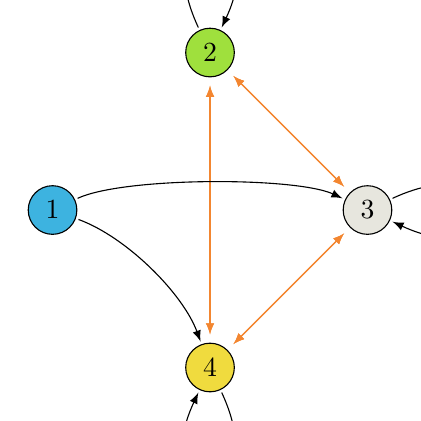
\begin{tikzpicture}
{ \definecolor{mycolor}{RGB}{61,179,224}
\node[hid, fill=mycolor] (1) at (180:2) {1};}
{ \definecolor{mycolor}{RGB}{159,224,61}
\node[hid, fill=mycolor] (2) at (90:2) {2};}
{ \definecolor{mycolor}{RGB}{231,230,222}
\node[hid, fill=mycolor] (3) at (0:2) {3};}
{ \definecolor{mycolor}{RGB}{240,219,62}
\node[hid, fill=mycolor] (4) at (-90:2) {4};}
\path[overlay,draw,pil] (1) .. controls +(25.00000:10.00000mm) and +(155.00000:10.00000mm) .. (3);
\path[overlay,draw,pil] (1) .. controls +(-20.00000:10.00000mm) and +(110.00000:10.00000mm) .. (4);
  \draw[pilip, on layer=back] (2) -- (3);
\path[overlay,draw,pil] (2) .. controls +(115.00000:20.00000mm) and +(65.00000:20.00000mm) .. (2);
  \draw[pilip, on layer=back] (2) -- (4);
\path[overlay,draw,pil] (3) .. controls +(25.00000:20.00000mm) and +(-25.00000:20.00000mm) .. (3);
  \draw[pilip, on layer=back] (3) -- (2);
  \draw[pilip, on layer=back] (3) -- (4);
  \draw[pilip, on layer=back] (4) -- (3);
  \draw[pilip, on layer=back] (4) -- (2);
\path[overlay,draw,pil] (4) .. controls +(-65.00000:20.00000mm) and +(-115.00000:20.00000mm) .. (4);

\end{tikzpicture}
};
& \node[scale=0.7](){
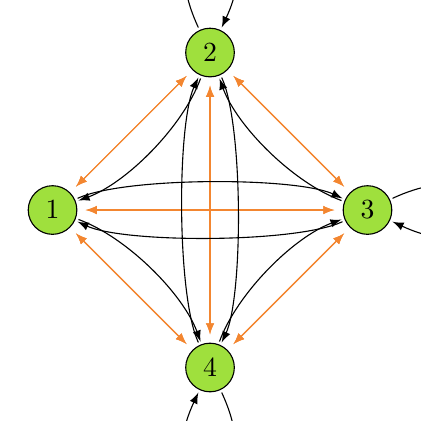
\begin{tikzpicture}
{ \definecolor{mycolor}{RGB}{159,224,61}
\node[hid, fill=mycolor] (1) at (180:2) {1};}
{ \definecolor{mycolor}{RGB}{159,224,61}
\node[hid, fill=mycolor] (2) at (90:2) {2};}
{ \definecolor{mycolor}{RGB}{159,224,61}
\node[hid, fill=mycolor] (3) at (0:2) {3};}
{ \definecolor{mycolor}{RGB}{159,224,61}
\node[hid, fill=mycolor] (4) at (-90:2) {4};}
  \draw[pilip, on layer=back] (1) -- (3);
\path[overlay,draw,pil] (1) .. controls +(25.00000:10.00000mm) and +(155.00000:10.00000mm) .. (3);
  \draw[pilip, on layer=back] (1) -- (2);
  \draw[pilip, on layer=back] (1) -- (4);
\path[overlay,draw,pil] (1) .. controls +(-20.00000:10.00000mm) and +(110.00000:10.00000mm) .. (4);
  \draw[pilip, on layer=back] (2) -- (1);
\path[overlay,draw,pil] (2) .. controls +(-110.00000:10.00000mm) and +(20.00000:10.00000mm) .. (1);
  \draw[pilip, on layer=back] (2) -- (3);
\path[overlay,draw,pil] (2) .. controls +(115.00000:20.00000mm) and +(65.00000:20.00000mm) .. (2);
  \draw[pilip, on layer=back] (2) -- (4);
\path[overlay,draw,pil] (2) .. controls +(-65.00000:10.00000mm) and +(65.00000:10.00000mm) .. (4);
  \draw[pilip, on layer=back] (3) -- (1);
\path[overlay,draw,pil] (3) .. controls +(205.00000:10.00000mm) and +(-25.00000:10.00000mm) .. (1);
\path[overlay,draw,pil] (3) .. controls +(25.00000:20.00000mm) and +(-25.00000:20.00000mm) .. (3);
  \draw[pilip, on layer=back] (3) -- (2);
\path[overlay,draw,pil] (3) .. controls +(160.00000:10.00000mm) and +(-70.00000:10.00000mm) .. (2);
  \draw[pilip, on layer=back] (3) -- (4);
  \draw[pilip, on layer=back] (4) -- (1);
  \draw[pilip, on layer=back] (4) -- (3);
\path[overlay,draw,pil] (4) .. controls +(70.00000:10.00000mm) and +(-160.00000:10.00000mm) .. (3);
  \draw[pilip, on layer=back] (4) -- (2);
\path[overlay,draw,pil] (4) .. controls +(115.00000:10.00000mm) and +(-115.00000:10.00000mm) .. (2);
\path[overlay,draw,pil] (4) .. controls +(-65.00000:20.00000mm) and +(-115.00000:20.00000mm) .. (4);

\end{tikzpicture}
};
& \node[scale=0.7](){
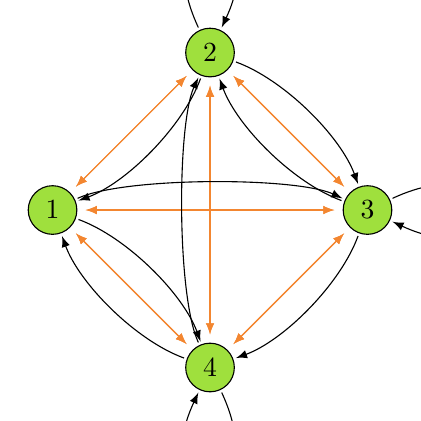
\begin{tikzpicture}
{ \definecolor{mycolor}{RGB}{159,224,61}
\node[hid, fill=mycolor] (1) at (180:2) {1};}
{ \definecolor{mycolor}{RGB}{159,224,61}
\node[hid, fill=mycolor] (2) at (90:2) {2};}
{ \definecolor{mycolor}{RGB}{159,224,61}
\node[hid, fill=mycolor] (3) at (0:2) {3};}
{ \definecolor{mycolor}{RGB}{159,224,61}
\node[hid, fill=mycolor] (4) at (-90:2) {4};}
  \draw[pilip, on layer=back] (1) -- (3);
\path[overlay,draw,pil] (1) .. controls +(25.00000:10.00000mm) and +(155.00000:10.00000mm) .. (3);
  \draw[pilip, on layer=back] (1) -- (2);
  \draw[pilip, on layer=back] (1) -- (4);
\path[overlay,draw,pil] (1) .. controls +(-20.00000:10.00000mm) and +(110.00000:10.00000mm) .. (4);
  \draw[pilip, on layer=back] (2) -- (1);
\path[overlay,draw,pil] (2) .. controls +(-110.00000:10.00000mm) and +(20.00000:10.00000mm) .. (1);
  \draw[pilip, on layer=back] (2) -- (3);
\path[overlay,draw,pil] (2) .. controls +(-20.00000:10.00000mm) and +(110.00000:10.00000mm) .. (3);
\path[overlay,draw,pil] (2) .. controls +(115.00000:20.00000mm) and +(65.00000:20.00000mm) .. (2);
  \draw[pilip, on layer=back] (2) -- (4);
  \draw[pilip, on layer=back] (3) -- (1);
\path[overlay,draw,pil] (3) .. controls +(25.00000:20.00000mm) and +(-25.00000:20.00000mm) .. (3);
  \draw[pilip, on layer=back] (3) -- (2);
\path[overlay,draw,pil] (3) .. controls +(160.00000:10.00000mm) and +(-70.00000:10.00000mm) .. (2);
  \draw[pilip, on layer=back] (3) -- (4);
\path[overlay,draw,pil] (3) .. controls +(-110.00000:10.00000mm) and +(20.00000:10.00000mm) .. (4);
  \draw[pilip, on layer=back] (4) -- (1);
\path[overlay,draw,pil] (4) .. controls +(160.00000:10.00000mm) and +(-70.00000:10.00000mm) .. (1);
  \draw[pilip, on layer=back] (4) -- (3);
  \draw[pilip, on layer=back] (4) -- (2);
\path[overlay,draw,pil] (4) .. controls +(115.00000:10.00000mm) and +(-115.00000:10.00000mm) .. (2);
\path[overlay,draw,pil] (4) .. controls +(-65.00000:20.00000mm) and +(-115.00000:20.00000mm) .. (4);

\end{tikzpicture}
};
& \node[scale=0.7](){
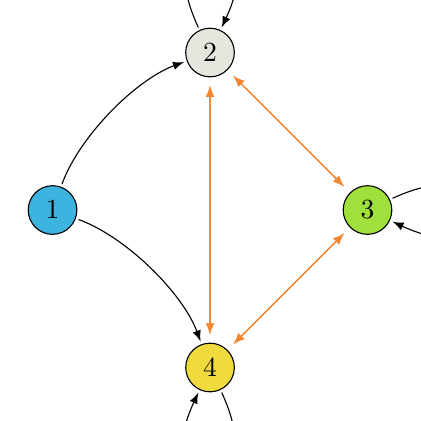
\begin{tikzpicture}
{ \definecolor{mycolor}{RGB}{61,179,224}
\node[hid, fill=mycolor] (1) at (180:2) {1};}
{ \definecolor{mycolor}{RGB}{231,230,222}
\node[hid, fill=mycolor] (2) at (90:2) {2};}
{ \definecolor{mycolor}{RGB}{159,224,61}
\node[hid, fill=mycolor] (3) at (0:2) {3};}
{ \definecolor{mycolor}{RGB}{240,219,62}
\node[hid, fill=mycolor] (4) at (-90:2) {4};}
\path[overlay,draw,pil] (1) .. controls +(70.00000:10.00000mm) and +(-160.00000:10.00000mm) .. (2);
\path[overlay,draw,pil] (1) .. controls +(-20.00000:10.00000mm) and +(110.00000:10.00000mm) .. (4);
  \draw[pilip, on layer=back] (2) -- (3);
\path[overlay,draw,pil] (2) .. controls +(115.00000:20.00000mm) and +(65.00000:20.00000mm) .. (2);
  \draw[pilip, on layer=back] (2) -- (4);
\path[overlay,draw,pil] (3) .. controls +(25.00000:20.00000mm) and +(-25.00000:20.00000mm) .. (3);
  \draw[pilip, on layer=back] (3) -- (2);
  \draw[pilip, on layer=back] (3) -- (4);
  \draw[pilip, on layer=back] (4) -- (3);
  \draw[pilip, on layer=back] (4) -- (2);
\path[overlay,draw,pil] (4) .. controls +(-65.00000:20.00000mm) and +(-115.00000:20.00000mm) .. (4);

\end{tikzpicture}
};
\\
  \node[scale=0.7](){
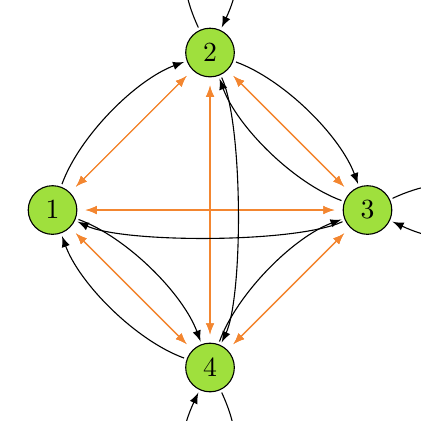
\begin{tikzpicture}
{ \definecolor{mycolor}{RGB}{159,224,61}
\node[hid, fill=mycolor] (1) at (180:2) {1};}
{ \definecolor{mycolor}{RGB}{159,224,61}
\node[hid, fill=mycolor] (2) at (90:2) {2};}
{ \definecolor{mycolor}{RGB}{159,224,61}
\node[hid, fill=mycolor] (3) at (0:2) {3};}
{ \definecolor{mycolor}{RGB}{159,224,61}
\node[hid, fill=mycolor] (4) at (-90:2) {4};}
  \draw[pilip, on layer=back] (1) -- (3);
  \draw[pilip, on layer=back] (1) -- (2);
\path[overlay,draw,pil] (1) .. controls +(70.00000:10.00000mm) and +(-160.00000:10.00000mm) .. (2);
  \draw[pilip, on layer=back] (1) -- (4);
\path[overlay,draw,pil] (1) .. controls +(-20.00000:10.00000mm) and +(110.00000:10.00000mm) .. (4);
  \draw[pilip, on layer=back] (2) -- (1);
  \draw[pilip, on layer=back] (2) -- (3);
\path[overlay,draw,pil] (2) .. controls +(-20.00000:10.00000mm) and +(110.00000:10.00000mm) .. (3);
\path[overlay,draw,pil] (2) .. controls +(115.00000:20.00000mm) and +(65.00000:20.00000mm) .. (2);
  \draw[pilip, on layer=back] (2) -- (4);
\path[overlay,draw,pil] (2) .. controls +(-65.00000:10.00000mm) and +(65.00000:10.00000mm) .. (4);
  \draw[pilip, on layer=back] (3) -- (1);
\path[overlay,draw,pil] (3) .. controls +(205.00000:10.00000mm) and +(-25.00000:10.00000mm) .. (1);
\path[overlay,draw,pil] (3) .. controls +(25.00000:20.00000mm) and +(-25.00000:20.00000mm) .. (3);
  \draw[pilip, on layer=back] (3) -- (2);
\path[overlay,draw,pil] (3) .. controls +(160.00000:10.00000mm) and +(-70.00000:10.00000mm) .. (2);
  \draw[pilip, on layer=back] (3) -- (4);
  \draw[pilip, on layer=back] (4) -- (1);
\path[overlay,draw,pil] (4) .. controls +(160.00000:10.00000mm) and +(-70.00000:10.00000mm) .. (1);
  \draw[pilip, on layer=back] (4) -- (3);
\path[overlay,draw,pil] (4) .. controls +(70.00000:10.00000mm) and +(-160.00000:10.00000mm) .. (3);
  \draw[pilip, on layer=back] (4) -- (2);
\path[overlay,draw,pil] (4) .. controls +(-65.00000:20.00000mm) and +(-115.00000:20.00000mm) .. (4);

\end{tikzpicture}
};
& \node[scale=0.7](){
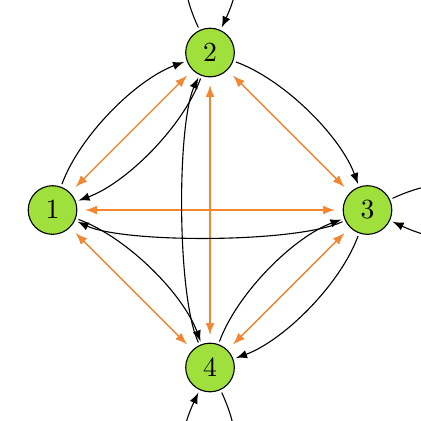
\begin{tikzpicture}
{ \definecolor{mycolor}{RGB}{159,224,61}
\node[hid, fill=mycolor] (1) at (180:2) {1};}
{ \definecolor{mycolor}{RGB}{159,224,61}
\node[hid, fill=mycolor] (2) at (90:2) {2};}
{ \definecolor{mycolor}{RGB}{159,224,61}
\node[hid, fill=mycolor] (3) at (0:2) {3};}
{ \definecolor{mycolor}{RGB}{159,224,61}
\node[hid, fill=mycolor] (4) at (-90:2) {4};}
  \draw[pilip, on layer=back] (1) -- (3);
  \draw[pilip, on layer=back] (1) -- (2);
\path[overlay,draw,pil] (1) .. controls +(70.00000:10.00000mm) and +(-160.00000:10.00000mm) .. (2);
  \draw[pilip, on layer=back] (1) -- (4);
\path[overlay,draw,pil] (1) .. controls +(-20.00000:10.00000mm) and +(110.00000:10.00000mm) .. (4);
  \draw[pilip, on layer=back] (2) -- (1);
\path[overlay,draw,pil] (2) .. controls +(-110.00000:10.00000mm) and +(20.00000:10.00000mm) .. (1);
  \draw[pilip, on layer=back] (2) -- (3);
\path[overlay,draw,pil] (2) .. controls +(-20.00000:10.00000mm) and +(110.00000:10.00000mm) .. (3);
\path[overlay,draw,pil] (2) .. controls +(115.00000:20.00000mm) and +(65.00000:20.00000mm) .. (2);
  \draw[pilip, on layer=back] (2) -- (4);
  \draw[pilip, on layer=back] (3) -- (1);
\path[overlay,draw,pil] (3) .. controls +(205.00000:10.00000mm) and +(-25.00000:10.00000mm) .. (1);
\path[overlay,draw,pil] (3) .. controls +(25.00000:20.00000mm) and +(-25.00000:20.00000mm) .. (3);
  \draw[pilip, on layer=back] (3) -- (2);
  \draw[pilip, on layer=back] (3) -- (4);
\path[overlay,draw,pil] (3) .. controls +(-110.00000:10.00000mm) and +(20.00000:10.00000mm) .. (4);
  \draw[pilip, on layer=back] (4) -- (1);
  \draw[pilip, on layer=back] (4) -- (3);
\path[overlay,draw,pil] (4) .. controls +(70.00000:10.00000mm) and +(-160.00000:10.00000mm) .. (3);
  \draw[pilip, on layer=back] (4) -- (2);
\path[overlay,draw,pil] (4) .. controls +(115.00000:10.00000mm) and +(-115.00000:10.00000mm) .. (2);
\path[overlay,draw,pil] (4) .. controls +(-65.00000:20.00000mm) and +(-115.00000:20.00000mm) .. (4);

\end{tikzpicture}
};
& \node[scale=0.7](){
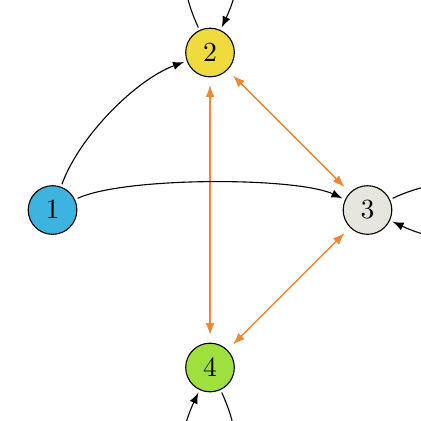
\begin{tikzpicture}
{ \definecolor{mycolor}{RGB}{61,179,224}
\node[hid, fill=mycolor] (1) at (180:2) {1};}
{ \definecolor{mycolor}{RGB}{240,219,62}
\node[hid, fill=mycolor] (2) at (90:2) {2};}
{ \definecolor{mycolor}{RGB}{231,230,222}
\node[hid, fill=mycolor] (3) at (0:2) {3};}
{ \definecolor{mycolor}{RGB}{159,224,61}
\node[hid, fill=mycolor] (4) at (-90:2) {4};}
\path[overlay,draw,pil] (1) .. controls +(25.00000:10.00000mm) and +(155.00000:10.00000mm) .. (3);
\path[overlay,draw,pil] (1) .. controls +(70.00000:10.00000mm) and +(-160.00000:10.00000mm) .. (2);
  \draw[pilip, on layer=back] (2) -- (3);
\path[overlay,draw,pil] (2) .. controls +(115.00000:20.00000mm) and +(65.00000:20.00000mm) .. (2);
  \draw[pilip, on layer=back] (2) -- (4);
\path[overlay,draw,pil] (3) .. controls +(25.00000:20.00000mm) and +(-25.00000:20.00000mm) .. (3);
  \draw[pilip, on layer=back] (3) -- (2);
  \draw[pilip, on layer=back] (3) -- (4);
  \draw[pilip, on layer=back] (4) -- (3);
  \draw[pilip, on layer=back] (4) -- (2);
\path[overlay,draw,pil] (4) .. controls +(-65.00000:20.00000mm) and +(-115.00000:20.00000mm) .. (4);

\end{tikzpicture}
};
& \node[scale=0.7](){
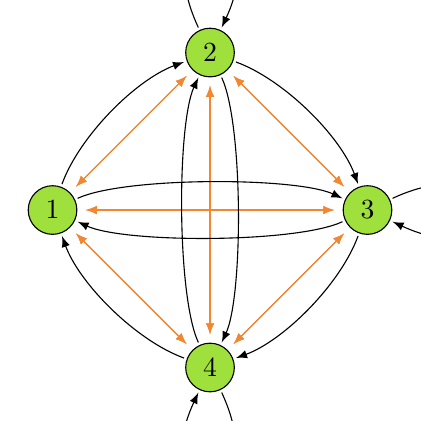
\begin{tikzpicture}
{ \definecolor{mycolor}{RGB}{159,224,61}
\node[hid, fill=mycolor] (1) at (180:2) {1};}
{ \definecolor{mycolor}{RGB}{159,224,61}
\node[hid, fill=mycolor] (2) at (90:2) {2};}
{ \definecolor{mycolor}{RGB}{159,224,61}
\node[hid, fill=mycolor] (3) at (0:2) {3};}
{ \definecolor{mycolor}{RGB}{159,224,61}
\node[hid, fill=mycolor] (4) at (-90:2) {4};}
  \draw[pilip, on layer=back] (1) -- (3);
\path[overlay,draw,pil] (1) .. controls +(25.00000:10.00000mm) and +(155.00000:10.00000mm) .. (3);
  \draw[pilip, on layer=back] (1) -- (2);
\path[overlay,draw,pil] (1) .. controls +(70.00000:10.00000mm) and +(-160.00000:10.00000mm) .. (2);
  \draw[pilip, on layer=back] (1) -- (4);
  \draw[pilip, on layer=back] (2) -- (1);
  \draw[pilip, on layer=back] (2) -- (3);
\path[overlay,draw,pil] (2) .. controls +(-20.00000:10.00000mm) and +(110.00000:10.00000mm) .. (3);
\path[overlay,draw,pil] (2) .. controls +(115.00000:20.00000mm) and +(65.00000:20.00000mm) .. (2);
  \draw[pilip, on layer=back] (2) -- (4);
\path[overlay,draw,pil] (2) .. controls +(-65.00000:10.00000mm) and +(65.00000:10.00000mm) .. (4);
  \draw[pilip, on layer=back] (3) -- (1);
\path[overlay,draw,pil] (3) .. controls +(205.00000:10.00000mm) and +(-25.00000:10.00000mm) .. (1);
\path[overlay,draw,pil] (3) .. controls +(25.00000:20.00000mm) and +(-25.00000:20.00000mm) .. (3);
  \draw[pilip, on layer=back] (3) -- (2);
  \draw[pilip, on layer=back] (3) -- (4);
\path[overlay,draw,pil] (3) .. controls +(-110.00000:10.00000mm) and +(20.00000:10.00000mm) .. (4);
  \draw[pilip, on layer=back] (4) -- (1);
\path[overlay,draw,pil] (4) .. controls +(160.00000:10.00000mm) and +(-70.00000:10.00000mm) .. (1);
  \draw[pilip, on layer=back] (4) -- (3);
  \draw[pilip, on layer=back] (4) -- (2);
\path[overlay,draw,pil] (4) .. controls +(115.00000:10.00000mm) and +(-115.00000:10.00000mm) .. (2);
\path[overlay,draw,pil] (4) .. controls +(-65.00000:20.00000mm) and +(-115.00000:20.00000mm) .. (4);

\end{tikzpicture}
};
& \node[scale=0.7](){
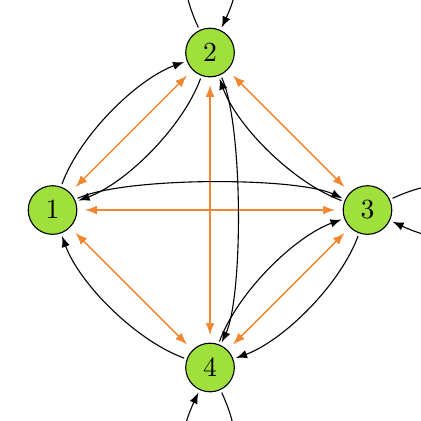
\begin{tikzpicture}
{ \definecolor{mycolor}{RGB}{159,224,61}
\node[hid, fill=mycolor] (1) at (180:2) {1};}
{ \definecolor{mycolor}{RGB}{159,224,61}
\node[hid, fill=mycolor] (2) at (90:2) {2};}
{ \definecolor{mycolor}{RGB}{159,224,61}
\node[hid, fill=mycolor] (3) at (0:2) {3};}
{ \definecolor{mycolor}{RGB}{159,224,61}
\node[hid, fill=mycolor] (4) at (-90:2) {4};}
  \draw[pilip, on layer=back] (1) -- (3);
\path[overlay,draw,pil] (1) .. controls +(25.00000:10.00000mm) and +(155.00000:10.00000mm) .. (3);
  \draw[pilip, on layer=back] (1) -- (2);
\path[overlay,draw,pil] (1) .. controls +(70.00000:10.00000mm) and +(-160.00000:10.00000mm) .. (2);
  \draw[pilip, on layer=back] (1) -- (4);
  \draw[pilip, on layer=back] (2) -- (1);
\path[overlay,draw,pil] (2) .. controls +(-110.00000:10.00000mm) and +(20.00000:10.00000mm) .. (1);
  \draw[pilip, on layer=back] (2) -- (3);
\path[overlay,draw,pil] (2) .. controls +(115.00000:20.00000mm) and +(65.00000:20.00000mm) .. (2);
  \draw[pilip, on layer=back] (2) -- (4);
\path[overlay,draw,pil] (2) .. controls +(-65.00000:10.00000mm) and +(65.00000:10.00000mm) .. (4);
  \draw[pilip, on layer=back] (3) -- (1);
\path[overlay,draw,pil] (3) .. controls +(25.00000:20.00000mm) and +(-25.00000:20.00000mm) .. (3);
  \draw[pilip, on layer=back] (3) -- (2);
\path[overlay,draw,pil] (3) .. controls +(160.00000:10.00000mm) and +(-70.00000:10.00000mm) .. (2);
  \draw[pilip, on layer=back] (3) -- (4);
\path[overlay,draw,pil] (3) .. controls +(-110.00000:10.00000mm) and +(20.00000:10.00000mm) .. (4);
  \draw[pilip, on layer=back] (4) -- (1);
\path[overlay,draw,pil] (4) .. controls +(160.00000:10.00000mm) and +(-70.00000:10.00000mm) .. (1);
  \draw[pilip, on layer=back] (4) -- (3);
\path[overlay,draw,pil] (4) .. controls +(70.00000:10.00000mm) and +(-160.00000:10.00000mm) .. (3);
  \draw[pilip, on layer=back] (4) -- (2);
\path[overlay,draw,pil] (4) .. controls +(-65.00000:20.00000mm) and +(-115.00000:20.00000mm) .. (4);

\end{tikzpicture}
};
\\
  \node[scale=0.7](){
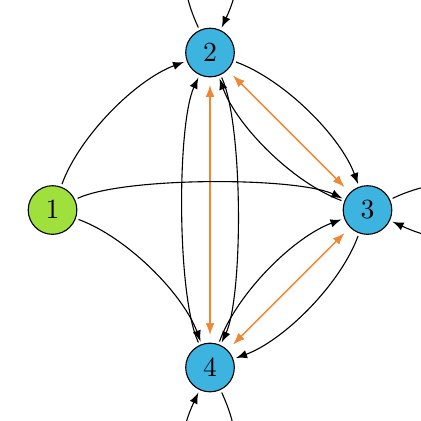
\begin{tikzpicture}
{ \definecolor{mycolor}{RGB}{159,224,61}
\node[hid, fill=mycolor] (1) at (180:2) {1};}
{ \definecolor{mycolor}{RGB}{61,179,224}
\node[hid, fill=mycolor] (2) at (90:2) {2};}
{ \definecolor{mycolor}{RGB}{61,179,224}
\node[hid, fill=mycolor] (3) at (0:2) {3};}
{ \definecolor{mycolor}{RGB}{61,179,224}
\node[hid, fill=mycolor] (4) at (-90:2) {4};}
\path[overlay,draw,pil] (1) .. controls +(25.00000:10.00000mm) and +(155.00000:10.00000mm) .. (3);
\path[overlay,draw,pil] (1) .. controls +(70.00000:10.00000mm) and +(-160.00000:10.00000mm) .. (2);
\path[overlay,draw,pil] (1) .. controls +(-20.00000:10.00000mm) and +(110.00000:10.00000mm) .. (4);
  \draw[pilip, on layer=back] (2) -- (3);
\path[overlay,draw,pil] (2) .. controls +(-20.00000:10.00000mm) and +(110.00000:10.00000mm) .. (3);
\path[overlay,draw,pil] (2) .. controls +(115.00000:20.00000mm) and +(65.00000:20.00000mm) .. (2);
  \draw[pilip, on layer=back] (2) -- (4);
\path[overlay,draw,pil] (2) .. controls +(-65.00000:10.00000mm) and +(65.00000:10.00000mm) .. (4);
\path[overlay,draw,pil] (3) .. controls +(25.00000:20.00000mm) and +(-25.00000:20.00000mm) .. (3);
  \draw[pilip, on layer=back] (3) -- (2);
\path[overlay,draw,pil] (3) .. controls +(160.00000:10.00000mm) and +(-70.00000:10.00000mm) .. (2);
  \draw[pilip, on layer=back] (3) -- (4);
\path[overlay,draw,pil] (3) .. controls +(-110.00000:10.00000mm) and +(20.00000:10.00000mm) .. (4);
  \draw[pilip, on layer=back] (4) -- (3);
\path[overlay,draw,pil] (4) .. controls +(70.00000:10.00000mm) and +(-160.00000:10.00000mm) .. (3);
  \draw[pilip, on layer=back] (4) -- (2);
\path[overlay,draw,pil] (4) .. controls +(115.00000:10.00000mm) and +(-115.00000:10.00000mm) .. (2);
\path[overlay,draw,pil] (4) .. controls +(-65.00000:20.00000mm) and +(-115.00000:20.00000mm) .. (4);

\end{tikzpicture}
};
& \node[scale=0.7](){
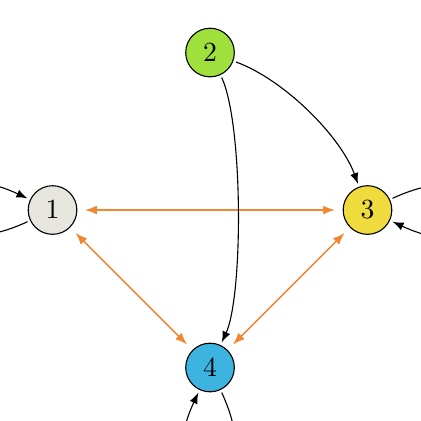
\begin{tikzpicture}
{ \definecolor{mycolor}{RGB}{231,230,222}
\node[hid, fill=mycolor] (1) at (180:2) {1};}
{ \definecolor{mycolor}{RGB}{159,224,61}
\node[hid, fill=mycolor] (2) at (90:2) {2};}
{ \definecolor{mycolor}{RGB}{240,219,62}
\node[hid, fill=mycolor] (3) at (0:2) {3};}
{ \definecolor{mycolor}{RGB}{61,179,224}
\node[hid, fill=mycolor] (4) at (-90:2) {4};}
\path[overlay,draw,pil] (1) .. controls +(205.00000:20.00000mm) and +(155.00000:20.00000mm) .. (1);
  \draw[pilip, on layer=back] (1) -- (3);
  \draw[pilip, on layer=back] (1) -- (4);
\path[overlay,draw,pil] (2) .. controls +(-20.00000:10.00000mm) and +(110.00000:10.00000mm) .. (3);
\path[overlay,draw,pil] (2) .. controls +(-65.00000:10.00000mm) and +(65.00000:10.00000mm) .. (4);
  \draw[pilip, on layer=back] (3) -- (1);
\path[overlay,draw,pil] (3) .. controls +(25.00000:20.00000mm) and +(-25.00000:20.00000mm) .. (3);
  \draw[pilip, on layer=back] (3) -- (4);
  \draw[pilip, on layer=back] (4) -- (1);
  \draw[pilip, on layer=back] (4) -- (3);
\path[overlay,draw,pil] (4) .. controls +(-65.00000:20.00000mm) and +(-115.00000:20.00000mm) .. (4);

\end{tikzpicture}
};
& \node[scale=0.7](){
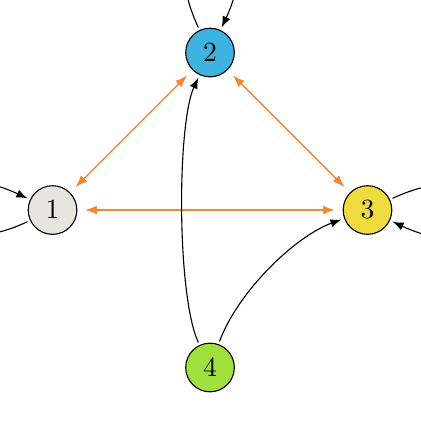
\begin{tikzpicture}
{ \definecolor{mycolor}{RGB}{231,230,222}
\node[hid, fill=mycolor] (1) at (180:2) {1};}
{ \definecolor{mycolor}{RGB}{61,179,224}
\node[hid, fill=mycolor] (2) at (90:2) {2};}
{ \definecolor{mycolor}{RGB}{240,219,62}
\node[hid, fill=mycolor] (3) at (0:2) {3};}
{ \definecolor{mycolor}{RGB}{159,224,61}
\node[hid, fill=mycolor] (4) at (-90:2) {4};}
\path[overlay,draw,pil] (1) .. controls +(205.00000:20.00000mm) and +(155.00000:20.00000mm) .. (1);
  \draw[pilip, on layer=back] (1) -- (3);
  \draw[pilip, on layer=back] (1) -- (2);
  \draw[pilip, on layer=back] (2) -- (1);
  \draw[pilip, on layer=back] (2) -- (3);
\path[overlay,draw,pil] (2) .. controls +(115.00000:20.00000mm) and +(65.00000:20.00000mm) .. (2);
  \draw[pilip, on layer=back] (3) -- (1);
\path[overlay,draw,pil] (3) .. controls +(25.00000:20.00000mm) and +(-25.00000:20.00000mm) .. (3);
  \draw[pilip, on layer=back] (3) -- (2);
\path[overlay,draw,pil] (4) .. controls +(70.00000:10.00000mm) and +(-160.00000:10.00000mm) .. (3);
\path[overlay,draw,pil] (4) .. controls +(115.00000:10.00000mm) and +(-115.00000:10.00000mm) .. (2);

\end{tikzpicture}
};
& \node[scale=0.7](){
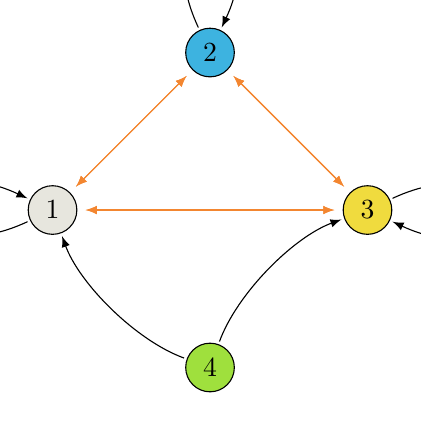
\begin{tikzpicture}
{ \definecolor{mycolor}{RGB}{231,230,222}
\node[hid, fill=mycolor] (1) at (180:2) {1};}
{ \definecolor{mycolor}{RGB}{61,179,224}
\node[hid, fill=mycolor] (2) at (90:2) {2};}
{ \definecolor{mycolor}{RGB}{240,219,62}
\node[hid, fill=mycolor] (3) at (0:2) {3};}
{ \definecolor{mycolor}{RGB}{159,224,61}
\node[hid, fill=mycolor] (4) at (-90:2) {4};}
\path[overlay,draw,pil] (1) .. controls +(205.00000:20.00000mm) and +(155.00000:20.00000mm) .. (1);
  \draw[pilip, on layer=back] (1) -- (3);
  \draw[pilip, on layer=back] (1) -- (2);
  \draw[pilip, on layer=back] (2) -- (1);
  \draw[pilip, on layer=back] (2) -- (3);
\path[overlay,draw,pil] (2) .. controls +(115.00000:20.00000mm) and +(65.00000:20.00000mm) .. (2);
  \draw[pilip, on layer=back] (3) -- (1);
\path[overlay,draw,pil] (3) .. controls +(25.00000:20.00000mm) and +(-25.00000:20.00000mm) .. (3);
  \draw[pilip, on layer=back] (3) -- (2);
\path[overlay,draw,pil] (4) .. controls +(160.00000:10.00000mm) and +(-70.00000:10.00000mm) .. (1);
\path[overlay,draw,pil] (4) .. controls +(70.00000:10.00000mm) and +(-160.00000:10.00000mm) .. (3);

\end{tikzpicture}
};
& \node[scale=0.7](){
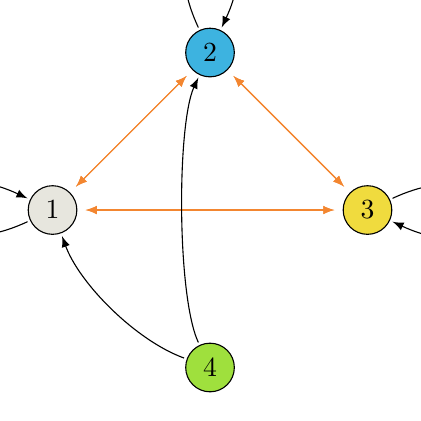
\begin{tikzpicture}
{ \definecolor{mycolor}{RGB}{231,230,222}
\node[hid, fill=mycolor] (1) at (180:2) {1};}
{ \definecolor{mycolor}{RGB}{61,179,224}
\node[hid, fill=mycolor] (2) at (90:2) {2};}
{ \definecolor{mycolor}{RGB}{240,219,62}
\node[hid, fill=mycolor] (3) at (0:2) {3};}
{ \definecolor{mycolor}{RGB}{159,224,61}
\node[hid, fill=mycolor] (4) at (-90:2) {4};}
\path[overlay,draw,pil] (1) .. controls +(205.00000:20.00000mm) and +(155.00000:20.00000mm) .. (1);
  \draw[pilip, on layer=back] (1) -- (3);
  \draw[pilip, on layer=back] (1) -- (2);
  \draw[pilip, on layer=back] (2) -- (1);
  \draw[pilip, on layer=back] (2) -- (3);
\path[overlay,draw,pil] (2) .. controls +(115.00000:20.00000mm) and +(65.00000:20.00000mm) .. (2);
  \draw[pilip, on layer=back] (3) -- (1);
\path[overlay,draw,pil] (3) .. controls +(25.00000:20.00000mm) and +(-25.00000:20.00000mm) .. (3);
  \draw[pilip, on layer=back] (3) -- (2);
\path[overlay,draw,pil] (4) .. controls +(160.00000:10.00000mm) and +(-70.00000:10.00000mm) .. (1);
\path[overlay,draw,pil] (4) .. controls +(115.00000:10.00000mm) and +(-115.00000:10.00000mm) .. (2);

\end{tikzpicture}
};
\\
  \node[scale=0.7](){
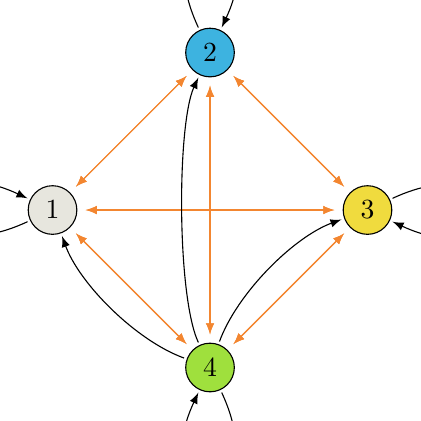
\begin{tikzpicture}
{ \definecolor{mycolor}{RGB}{231,230,222}
\node[hid, fill=mycolor] (1) at (180:2) {1};}
{ \definecolor{mycolor}{RGB}{61,179,224}
\node[hid, fill=mycolor] (2) at (90:2) {2};}
{ \definecolor{mycolor}{RGB}{240,219,62}
\node[hid, fill=mycolor] (3) at (0:2) {3};}
{ \definecolor{mycolor}{RGB}{159,224,61}
\node[hid, fill=mycolor] (4) at (-90:2) {4};}
\path[overlay,draw,pil] (1) .. controls +(205.00000:20.00000mm) and +(155.00000:20.00000mm) .. (1);
  \draw[pilip, on layer=back] (1) -- (3);
  \draw[pilip, on layer=back] (1) -- (2);
  \draw[pilip, on layer=back] (1) -- (4);
  \draw[pilip, on layer=back] (2) -- (1);
  \draw[pilip, on layer=back] (2) -- (3);
\path[overlay,draw,pil] (2) .. controls +(115.00000:20.00000mm) and +(65.00000:20.00000mm) .. (2);
  \draw[pilip, on layer=back] (2) -- (4);
  \draw[pilip, on layer=back] (3) -- (1);
\path[overlay,draw,pil] (3) .. controls +(25.00000:20.00000mm) and +(-25.00000:20.00000mm) .. (3);
  \draw[pilip, on layer=back] (3) -- (2);
  \draw[pilip, on layer=back] (3) -- (4);
  \draw[pilip, on layer=back] (4) -- (1);
\path[overlay,draw,pil] (4) .. controls +(160.00000:10.00000mm) and +(-70.00000:10.00000mm) .. (1);
  \draw[pilip, on layer=back] (4) -- (3);
\path[overlay,draw,pil] (4) .. controls +(70.00000:10.00000mm) and +(-160.00000:10.00000mm) .. (3);
  \draw[pilip, on layer=back] (4) -- (2);
\path[overlay,draw,pil] (4) .. controls +(115.00000:10.00000mm) and +(-115.00000:10.00000mm) .. (2);
\path[overlay,draw,pil] (4) .. controls +(-65.00000:20.00000mm) and +(-115.00000:20.00000mm) .. (4);

\end{tikzpicture}
};
& \node[scale=0.7](){
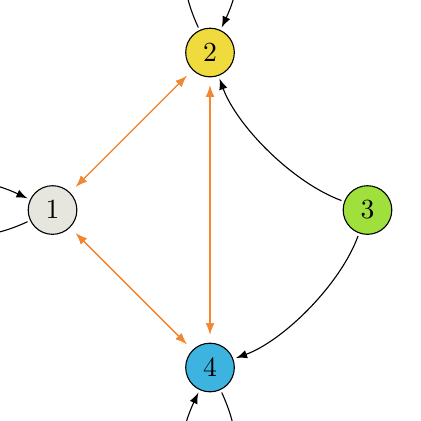
\begin{tikzpicture}
{ \definecolor{mycolor}{RGB}{231,230,222}
\node[hid, fill=mycolor] (1) at (180:2) {1};}
{ \definecolor{mycolor}{RGB}{240,219,62}
\node[hid, fill=mycolor] (2) at (90:2) {2};}
{ \definecolor{mycolor}{RGB}{159,224,61}
\node[hid, fill=mycolor] (3) at (0:2) {3};}
{ \definecolor{mycolor}{RGB}{61,179,224}
\node[hid, fill=mycolor] (4) at (-90:2) {4};}
\path[overlay,draw,pil] (1) .. controls +(205.00000:20.00000mm) and +(155.00000:20.00000mm) .. (1);
  \draw[pilip, on layer=back] (1) -- (2);
  \draw[pilip, on layer=back] (1) -- (4);
  \draw[pilip, on layer=back] (2) -- (1);
\path[overlay,draw,pil] (2) .. controls +(115.00000:20.00000mm) and +(65.00000:20.00000mm) .. (2);
  \draw[pilip, on layer=back] (2) -- (4);
\path[overlay,draw,pil] (3) .. controls +(160.00000:10.00000mm) and +(-70.00000:10.00000mm) .. (2);
\path[overlay,draw,pil] (3) .. controls +(-110.00000:10.00000mm) and +(20.00000:10.00000mm) .. (4);
  \draw[pilip, on layer=back] (4) -- (1);
  \draw[pilip, on layer=back] (4) -- (2);
\path[overlay,draw,pil] (4) .. controls +(-65.00000:20.00000mm) and +(-115.00000:20.00000mm) .. (4);

\end{tikzpicture}
};
& \node[scale=0.7](){
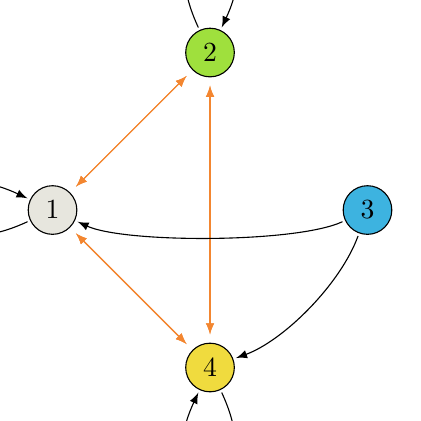
\begin{tikzpicture}
{ \definecolor{mycolor}{RGB}{231,230,222}
\node[hid, fill=mycolor] (1) at (180:2) {1};}
{ \definecolor{mycolor}{RGB}{159,224,61}
\node[hid, fill=mycolor] (2) at (90:2) {2};}
{ \definecolor{mycolor}{RGB}{61,179,224}
\node[hid, fill=mycolor] (3) at (0:2) {3};}
{ \definecolor{mycolor}{RGB}{240,219,62}
\node[hid, fill=mycolor] (4) at (-90:2) {4};}
\path[overlay,draw,pil] (1) .. controls +(205.00000:20.00000mm) and +(155.00000:20.00000mm) .. (1);
  \draw[pilip, on layer=back] (1) -- (2);
  \draw[pilip, on layer=back] (1) -- (4);
  \draw[pilip, on layer=back] (2) -- (1);
\path[overlay,draw,pil] (2) .. controls +(115.00000:20.00000mm) and +(65.00000:20.00000mm) .. (2);
  \draw[pilip, on layer=back] (2) -- (4);
\path[overlay,draw,pil] (3) .. controls +(205.00000:10.00000mm) and +(-25.00000:10.00000mm) .. (1);
\path[overlay,draw,pil] (3) .. controls +(-110.00000:10.00000mm) and +(20.00000:10.00000mm) .. (4);
  \draw[pilip, on layer=back] (4) -- (1);
  \draw[pilip, on layer=back] (4) -- (2);
\path[overlay,draw,pil] (4) .. controls +(-65.00000:20.00000mm) and +(-115.00000:20.00000mm) .. (4);

\end{tikzpicture}
};
& \node[scale=0.7](){
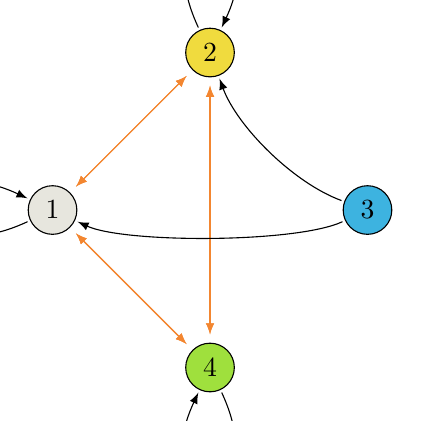
\begin{tikzpicture}
{ \definecolor{mycolor}{RGB}{231,230,222}
\node[hid, fill=mycolor] (1) at (180:2) {1};}
{ \definecolor{mycolor}{RGB}{240,219,62}
\node[hid, fill=mycolor] (2) at (90:2) {2};}
{ \definecolor{mycolor}{RGB}{61,179,224}
\node[hid, fill=mycolor] (3) at (0:2) {3};}
{ \definecolor{mycolor}{RGB}{159,224,61}
\node[hid, fill=mycolor] (4) at (-90:2) {4};}
\path[overlay,draw,pil] (1) .. controls +(205.00000:20.00000mm) and +(155.00000:20.00000mm) .. (1);
  \draw[pilip, on layer=back] (1) -- (2);
  \draw[pilip, on layer=back] (1) -- (4);
  \draw[pilip, on layer=back] (2) -- (1);
\path[overlay,draw,pil] (2) .. controls +(115.00000:20.00000mm) and +(65.00000:20.00000mm) .. (2);
  \draw[pilip, on layer=back] (2) -- (4);
\path[overlay,draw,pil] (3) .. controls +(205.00000:10.00000mm) and +(-25.00000:10.00000mm) .. (1);
\path[overlay,draw,pil] (3) .. controls +(160.00000:10.00000mm) and +(-70.00000:10.00000mm) .. (2);
  \draw[pilip, on layer=back] (4) -- (1);
  \draw[pilip, on layer=back] (4) -- (2);
\path[overlay,draw,pil] (4) .. controls +(-65.00000:20.00000mm) and +(-115.00000:20.00000mm) .. (4);

\end{tikzpicture}
};
& \node[scale=0.7](){
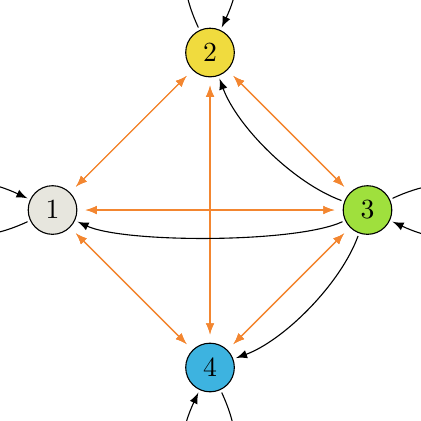
\begin{tikzpicture}
{ \definecolor{mycolor}{RGB}{231,230,222}
\node[hid, fill=mycolor] (1) at (180:2) {1};}
{ \definecolor{mycolor}{RGB}{240,219,62}
\node[hid, fill=mycolor] (2) at (90:2) {2};}
{ \definecolor{mycolor}{RGB}{159,224,61}
\node[hid, fill=mycolor] (3) at (0:2) {3};}
{ \definecolor{mycolor}{RGB}{61,179,224}
\node[hid, fill=mycolor] (4) at (-90:2) {4};}
\path[overlay,draw,pil] (1) .. controls +(205.00000:20.00000mm) and +(155.00000:20.00000mm) .. (1);
  \draw[pilip, on layer=back] (1) -- (3);
  \draw[pilip, on layer=back] (1) -- (2);
  \draw[pilip, on layer=back] (1) -- (4);
  \draw[pilip, on layer=back] (2) -- (1);
  \draw[pilip, on layer=back] (2) -- (3);
\path[overlay,draw,pil] (2) .. controls +(115.00000:20.00000mm) and +(65.00000:20.00000mm) .. (2);
  \draw[pilip, on layer=back] (2) -- (4);
  \draw[pilip, on layer=back] (3) -- (1);
\path[overlay,draw,pil] (3) .. controls +(205.00000:10.00000mm) and +(-25.00000:10.00000mm) .. (1);
\path[overlay,draw,pil] (3) .. controls +(25.00000:20.00000mm) and +(-25.00000:20.00000mm) .. (3);
  \draw[pilip, on layer=back] (3) -- (2);
\path[overlay,draw,pil] (3) .. controls +(160.00000:10.00000mm) and +(-70.00000:10.00000mm) .. (2);
  \draw[pilip, on layer=back] (3) -- (4);
\path[overlay,draw,pil] (3) .. controls +(-110.00000:10.00000mm) and +(20.00000:10.00000mm) .. (4);
  \draw[pilip, on layer=back] (4) -- (1);
  \draw[pilip, on layer=back] (4) -- (3);
  \draw[pilip, on layer=back] (4) -- (2);
\path[overlay,draw,pil] (4) .. controls +(-65.00000:20.00000mm) and +(-115.00000:20.00000mm) .. (4);

\end{tikzpicture}
};
\\
  \node[scale=0.7](){
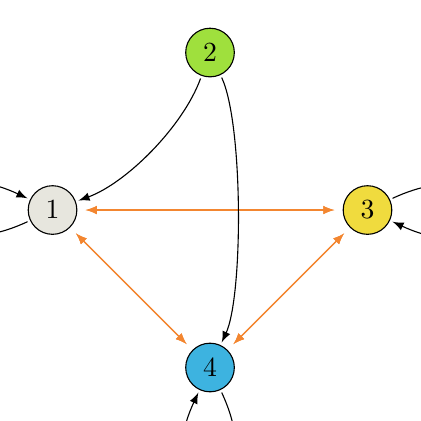
\begin{tikzpicture}
{ \definecolor{mycolor}{RGB}{231,230,222}
\node[hid, fill=mycolor] (1) at (180:2) {1};}
{ \definecolor{mycolor}{RGB}{159,224,61}
\node[hid, fill=mycolor] (2) at (90:2) {2};}
{ \definecolor{mycolor}{RGB}{240,219,62}
\node[hid, fill=mycolor] (3) at (0:2) {3};}
{ \definecolor{mycolor}{RGB}{61,179,224}
\node[hid, fill=mycolor] (4) at (-90:2) {4};}
\path[overlay,draw,pil] (1) .. controls +(205.00000:20.00000mm) and +(155.00000:20.00000mm) .. (1);
  \draw[pilip, on layer=back] (1) -- (3);
  \draw[pilip, on layer=back] (1) -- (4);
\path[overlay,draw,pil] (2) .. controls +(-110.00000:10.00000mm) and +(20.00000:10.00000mm) .. (1);
\path[overlay,draw,pil] (2) .. controls +(-65.00000:10.00000mm) and +(65.00000:10.00000mm) .. (4);
  \draw[pilip, on layer=back] (3) -- (1);
\path[overlay,draw,pil] (3) .. controls +(25.00000:20.00000mm) and +(-25.00000:20.00000mm) .. (3);
  \draw[pilip, on layer=back] (3) -- (4);
  \draw[pilip, on layer=back] (4) -- (1);
  \draw[pilip, on layer=back] (4) -- (3);
\path[overlay,draw,pil] (4) .. controls +(-65.00000:20.00000mm) and +(-115.00000:20.00000mm) .. (4);

\end{tikzpicture}
};
& \node[scale=0.7](){
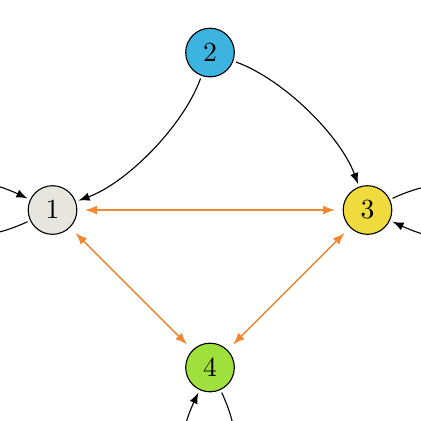
\begin{tikzpicture}
{ \definecolor{mycolor}{RGB}{231,230,222}
\node[hid, fill=mycolor] (1) at (180:2) {1};}
{ \definecolor{mycolor}{RGB}{61,179,224}
\node[hid, fill=mycolor] (2) at (90:2) {2};}
{ \definecolor{mycolor}{RGB}{240,219,62}
\node[hid, fill=mycolor] (3) at (0:2) {3};}
{ \definecolor{mycolor}{RGB}{159,224,61}
\node[hid, fill=mycolor] (4) at (-90:2) {4};}
\path[overlay,draw,pil] (1) .. controls +(205.00000:20.00000mm) and +(155.00000:20.00000mm) .. (1);
  \draw[pilip, on layer=back] (1) -- (3);
  \draw[pilip, on layer=back] (1) -- (4);
\path[overlay,draw,pil] (2) .. controls +(-110.00000:10.00000mm) and +(20.00000:10.00000mm) .. (1);
\path[overlay,draw,pil] (2) .. controls +(-20.00000:10.00000mm) and +(110.00000:10.00000mm) .. (3);
  \draw[pilip, on layer=back] (3) -- (1);
\path[overlay,draw,pil] (3) .. controls +(25.00000:20.00000mm) and +(-25.00000:20.00000mm) .. (3);
  \draw[pilip, on layer=back] (3) -- (4);
  \draw[pilip, on layer=back] (4) -- (1);
  \draw[pilip, on layer=back] (4) -- (3);
\path[overlay,draw,pil] (4) .. controls +(-65.00000:20.00000mm) and +(-115.00000:20.00000mm) .. (4);

\end{tikzpicture}
};
& \node[scale=0.7](){
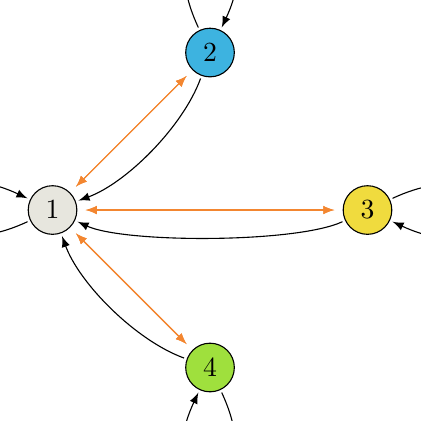
\begin{tikzpicture}
{ \definecolor{mycolor}{RGB}{231,230,222}
\node[hid, fill=mycolor] (1) at (180:2) {1};}
{ \definecolor{mycolor}{RGB}{61,179,224}
\node[hid, fill=mycolor] (2) at (90:2) {2};}
{ \definecolor{mycolor}{RGB}{240,219,62}
\node[hid, fill=mycolor] (3) at (0:2) {3};}
{ \definecolor{mycolor}{RGB}{159,224,61}
\node[hid, fill=mycolor] (4) at (-90:2) {4};}
\path[overlay,draw,pil] (1) .. controls +(205.00000:20.00000mm) and +(155.00000:20.00000mm) .. (1);
  \draw[pilip, on layer=back] (1) -- (3);
  \draw[pilip, on layer=back] (1) -- (2);
  \draw[pilip, on layer=back] (1) -- (4);
  \draw[pilip, on layer=back] (2) -- (1);
\path[overlay,draw,pil] (2) .. controls +(-110.00000:10.00000mm) and +(20.00000:10.00000mm) .. (1);
\path[overlay,draw,pil] (2) .. controls +(115.00000:20.00000mm) and +(65.00000:20.00000mm) .. (2);
  \draw[pilip, on layer=back] (3) -- (1);
\path[overlay,draw,pil] (3) .. controls +(205.00000:10.00000mm) and +(-25.00000:10.00000mm) .. (1);
\path[overlay,draw,pil] (3) .. controls +(25.00000:20.00000mm) and +(-25.00000:20.00000mm) .. (3);
  \draw[pilip, on layer=back] (4) -- (1);
\path[overlay,draw,pil] (4) .. controls +(160.00000:10.00000mm) and +(-70.00000:10.00000mm) .. (1);
\path[overlay,draw,pil] (4) .. controls +(-65.00000:20.00000mm) and +(-115.00000:20.00000mm) .. (4);

\end{tikzpicture}
};
& \node[scale=0.7](){
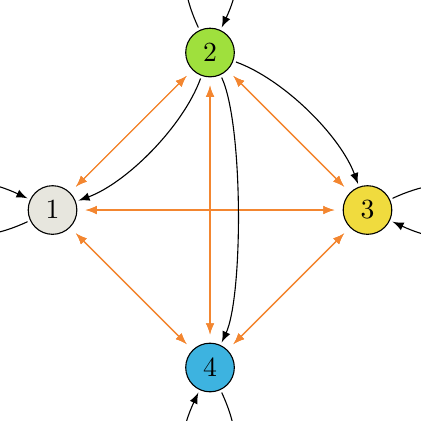
\begin{tikzpicture}
{ \definecolor{mycolor}{RGB}{231,230,222}
\node[hid, fill=mycolor] (1) at (180:2) {1};}
{ \definecolor{mycolor}{RGB}{159,224,61}
\node[hid, fill=mycolor] (2) at (90:2) {2};}
{ \definecolor{mycolor}{RGB}{240,219,62}
\node[hid, fill=mycolor] (3) at (0:2) {3};}
{ \definecolor{mycolor}{RGB}{61,179,224}
\node[hid, fill=mycolor] (4) at (-90:2) {4};}
\path[overlay,draw,pil] (1) .. controls +(205.00000:20.00000mm) and +(155.00000:20.00000mm) .. (1);
  \draw[pilip, on layer=back] (1) -- (3);
  \draw[pilip, on layer=back] (1) -- (2);
  \draw[pilip, on layer=back] (1) -- (4);
  \draw[pilip, on layer=back] (2) -- (1);
\path[overlay,draw,pil] (2) .. controls +(-110.00000:10.00000mm) and +(20.00000:10.00000mm) .. (1);
  \draw[pilip, on layer=back] (2) -- (3);
\path[overlay,draw,pil] (2) .. controls +(-20.00000:10.00000mm) and +(110.00000:10.00000mm) .. (3);
\path[overlay,draw,pil] (2) .. controls +(115.00000:20.00000mm) and +(65.00000:20.00000mm) .. (2);
  \draw[pilip, on layer=back] (2) -- (4);
\path[overlay,draw,pil] (2) .. controls +(-65.00000:10.00000mm) and +(65.00000:10.00000mm) .. (4);
  \draw[pilip, on layer=back] (3) -- (1);
\path[overlay,draw,pil] (3) .. controls +(25.00000:20.00000mm) and +(-25.00000:20.00000mm) .. (3);
  \draw[pilip, on layer=back] (3) -- (2);
  \draw[pilip, on layer=back] (3) -- (4);
  \draw[pilip, on layer=back] (4) -- (1);
  \draw[pilip, on layer=back] (4) -- (3);
  \draw[pilip, on layer=back] (4) -- (2);
\path[overlay,draw,pil] (4) .. controls +(-65.00000:20.00000mm) and +(-115.00000:20.00000mm) .. (4);

\end{tikzpicture}
};
& \node[scale=0.7](){
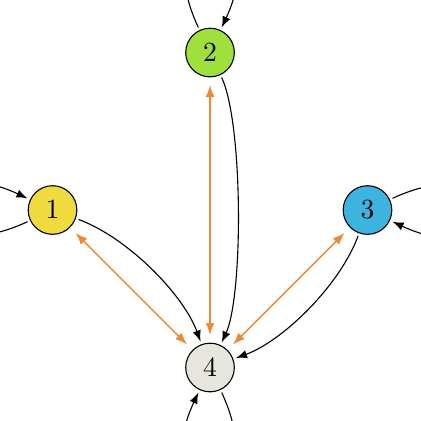
\begin{tikzpicture}
{ \definecolor{mycolor}{RGB}{240,219,62}
\node[hid, fill=mycolor] (1) at (180:2) {1};}
{ \definecolor{mycolor}{RGB}{159,224,61}
\node[hid, fill=mycolor] (2) at (90:2) {2};}
{ \definecolor{mycolor}{RGB}{61,179,224}
\node[hid, fill=mycolor] (3) at (0:2) {3};}
{ \definecolor{mycolor}{RGB}{231,230,222}
\node[hid, fill=mycolor] (4) at (-90:2) {4};}
\path[overlay,draw,pil] (1) .. controls +(205.00000:20.00000mm) and +(155.00000:20.00000mm) .. (1);
  \draw[pilip, on layer=back] (1) -- (4);
\path[overlay,draw,pil] (1) .. controls +(-20.00000:10.00000mm) and +(110.00000:10.00000mm) .. (4);
\path[overlay,draw,pil] (2) .. controls +(115.00000:20.00000mm) and +(65.00000:20.00000mm) .. (2);
  \draw[pilip, on layer=back] (2) -- (4);
\path[overlay,draw,pil] (2) .. controls +(-65.00000:10.00000mm) and +(65.00000:10.00000mm) .. (4);
\path[overlay,draw,pil] (3) .. controls +(25.00000:20.00000mm) and +(-25.00000:20.00000mm) .. (3);
  \draw[pilip, on layer=back] (3) -- (4);
\path[overlay,draw,pil] (3) .. controls +(-110.00000:10.00000mm) and +(20.00000:10.00000mm) .. (4);
  \draw[pilip, on layer=back] (4) -- (1);
  \draw[pilip, on layer=back] (4) -- (3);
  \draw[pilip, on layer=back] (4) -- (2);
\path[overlay,draw,pil] (4) .. controls +(-65.00000:20.00000mm) and +(-115.00000:20.00000mm) .. (4);

\end{tikzpicture}
};
\\
  \node[scale=0.7](){
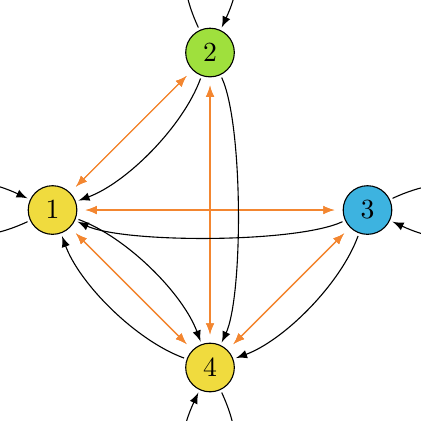
\begin{tikzpicture}
{ \definecolor{mycolor}{RGB}{240,219,62}
\node[hid, fill=mycolor] (1) at (180:2) {1};}
{ \definecolor{mycolor}{RGB}{159,224,61}
\node[hid, fill=mycolor] (2) at (90:2) {2};}
{ \definecolor{mycolor}{RGB}{61,179,224}
\node[hid, fill=mycolor] (3) at (0:2) {3};}
{ \definecolor{mycolor}{RGB}{240,219,62}
\node[hid, fill=mycolor] (4) at (-90:2) {4};}
\path[overlay,draw,pil] (1) .. controls +(205.00000:20.00000mm) and +(155.00000:20.00000mm) .. (1);
  \draw[pilip, on layer=back] (1) -- (3);
  \draw[pilip, on layer=back] (1) -- (2);
  \draw[pilip, on layer=back] (1) -- (4);
\path[overlay,draw,pil] (1) .. controls +(-20.00000:10.00000mm) and +(110.00000:10.00000mm) .. (4);
  \draw[pilip, on layer=back] (2) -- (1);
\path[overlay,draw,pil] (2) .. controls +(-110.00000:10.00000mm) and +(20.00000:10.00000mm) .. (1);
\path[overlay,draw,pil] (2) .. controls +(115.00000:20.00000mm) and +(65.00000:20.00000mm) .. (2);
  \draw[pilip, on layer=back] (2) -- (4);
\path[overlay,draw,pil] (2) .. controls +(-65.00000:10.00000mm) and +(65.00000:10.00000mm) .. (4);
  \draw[pilip, on layer=back] (3) -- (1);
\path[overlay,draw,pil] (3) .. controls +(205.00000:10.00000mm) and +(-25.00000:10.00000mm) .. (1);
\path[overlay,draw,pil] (3) .. controls +(25.00000:20.00000mm) and +(-25.00000:20.00000mm) .. (3);
  \draw[pilip, on layer=back] (3) -- (4);
\path[overlay,draw,pil] (3) .. controls +(-110.00000:10.00000mm) and +(20.00000:10.00000mm) .. (4);
  \draw[pilip, on layer=back] (4) -- (1);
\path[overlay,draw,pil] (4) .. controls +(160.00000:10.00000mm) and +(-70.00000:10.00000mm) .. (1);
  \draw[pilip, on layer=back] (4) -- (3);
  \draw[pilip, on layer=back] (4) -- (2);
\path[overlay,draw,pil] (4) .. controls +(-65.00000:20.00000mm) and +(-115.00000:20.00000mm) .. (4);

\end{tikzpicture}
};
& \node[scale=0.7](){
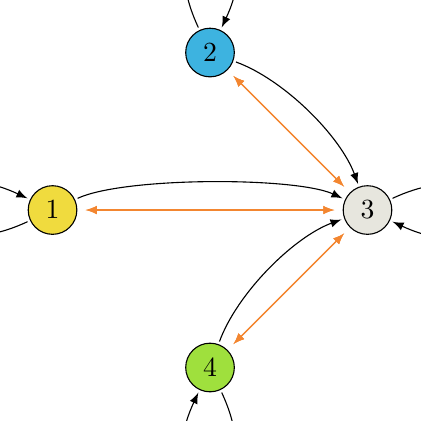
\begin{tikzpicture}
{ \definecolor{mycolor}{RGB}{240,219,62}
\node[hid, fill=mycolor] (1) at (180:2) {1};}
{ \definecolor{mycolor}{RGB}{61,179,224}
\node[hid, fill=mycolor] (2) at (90:2) {2};}
{ \definecolor{mycolor}{RGB}{231,230,222}
\node[hid, fill=mycolor] (3) at (0:2) {3};}
{ \definecolor{mycolor}{RGB}{159,224,61}
\node[hid, fill=mycolor] (4) at (-90:2) {4};}
\path[overlay,draw,pil] (1) .. controls +(205.00000:20.00000mm) and +(155.00000:20.00000mm) .. (1);
  \draw[pilip, on layer=back] (1) -- (3);
\path[overlay,draw,pil] (1) .. controls +(25.00000:10.00000mm) and +(155.00000:10.00000mm) .. (3);
  \draw[pilip, on layer=back] (2) -- (3);
\path[overlay,draw,pil] (2) .. controls +(-20.00000:10.00000mm) and +(110.00000:10.00000mm) .. (3);
\path[overlay,draw,pil] (2) .. controls +(115.00000:20.00000mm) and +(65.00000:20.00000mm) .. (2);
  \draw[pilip, on layer=back] (3) -- (1);
\path[overlay,draw,pil] (3) .. controls +(25.00000:20.00000mm) and +(-25.00000:20.00000mm) .. (3);
  \draw[pilip, on layer=back] (3) -- (2);
  \draw[pilip, on layer=back] (3) -- (4);
  \draw[pilip, on layer=back] (4) -- (3);
\path[overlay,draw,pil] (4) .. controls +(70.00000:10.00000mm) and +(-160.00000:10.00000mm) .. (3);
\path[overlay,draw,pil] (4) .. controls +(-65.00000:20.00000mm) and +(-115.00000:20.00000mm) .. (4);

\end{tikzpicture}
};
& \node[scale=0.7](){
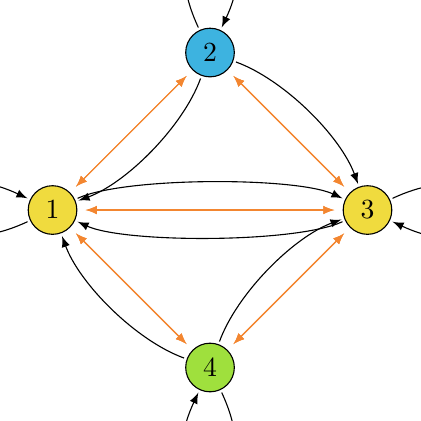
\begin{tikzpicture}
{ \definecolor{mycolor}{RGB}{240,219,62}
\node[hid, fill=mycolor] (1) at (180:2) {1};}
{ \definecolor{mycolor}{RGB}{61,179,224}
\node[hid, fill=mycolor] (2) at (90:2) {2};}
{ \definecolor{mycolor}{RGB}{240,219,62}
\node[hid, fill=mycolor] (3) at (0:2) {3};}
{ \definecolor{mycolor}{RGB}{159,224,61}
\node[hid, fill=mycolor] (4) at (-90:2) {4};}
\path[overlay,draw,pil] (1) .. controls +(205.00000:20.00000mm) and +(155.00000:20.00000mm) .. (1);
  \draw[pilip, on layer=back] (1) -- (3);
\path[overlay,draw,pil] (1) .. controls +(25.00000:10.00000mm) and +(155.00000:10.00000mm) .. (3);
  \draw[pilip, on layer=back] (1) -- (2);
  \draw[pilip, on layer=back] (1) -- (4);
  \draw[pilip, on layer=back] (2) -- (1);
\path[overlay,draw,pil] (2) .. controls +(-110.00000:10.00000mm) and +(20.00000:10.00000mm) .. (1);
  \draw[pilip, on layer=back] (2) -- (3);
\path[overlay,draw,pil] (2) .. controls +(-20.00000:10.00000mm) and +(110.00000:10.00000mm) .. (3);
\path[overlay,draw,pil] (2) .. controls +(115.00000:20.00000mm) and +(65.00000:20.00000mm) .. (2);
  \draw[pilip, on layer=back] (3) -- (1);
\path[overlay,draw,pil] (3) .. controls +(205.00000:10.00000mm) and +(-25.00000:10.00000mm) .. (1);
\path[overlay,draw,pil] (3) .. controls +(25.00000:20.00000mm) and +(-25.00000:20.00000mm) .. (3);
  \draw[pilip, on layer=back] (3) -- (2);
  \draw[pilip, on layer=back] (3) -- (4);
  \draw[pilip, on layer=back] (4) -- (1);
\path[overlay,draw,pil] (4) .. controls +(160.00000:10.00000mm) and +(-70.00000:10.00000mm) .. (1);
  \draw[pilip, on layer=back] (4) -- (3);
\path[overlay,draw,pil] (4) .. controls +(70.00000:10.00000mm) and +(-160.00000:10.00000mm) .. (3);
\path[overlay,draw,pil] (4) .. controls +(-65.00000:20.00000mm) and +(-115.00000:20.00000mm) .. (4);

\end{tikzpicture}
};
& \node[scale=0.7](){
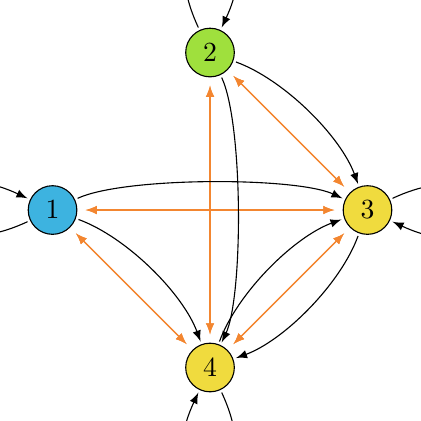
\begin{tikzpicture}
{ \definecolor{mycolor}{RGB}{61,179,224}
\node[hid, fill=mycolor] (1) at (180:2) {1};}
{ \definecolor{mycolor}{RGB}{159,224,61}
\node[hid, fill=mycolor] (2) at (90:2) {2};}
{ \definecolor{mycolor}{RGB}{240,219,62}
\node[hid, fill=mycolor] (3) at (0:2) {3};}
{ \definecolor{mycolor}{RGB}{240,219,62}
\node[hid, fill=mycolor] (4) at (-90:2) {4};}
\path[overlay,draw,pil] (1) .. controls +(205.00000:20.00000mm) and +(155.00000:20.00000mm) .. (1);
  \draw[pilip, on layer=back] (1) -- (3);
\path[overlay,draw,pil] (1) .. controls +(25.00000:10.00000mm) and +(155.00000:10.00000mm) .. (3);
  \draw[pilip, on layer=back] (1) -- (4);
\path[overlay,draw,pil] (1) .. controls +(-20.00000:10.00000mm) and +(110.00000:10.00000mm) .. (4);
  \draw[pilip, on layer=back] (2) -- (3);
\path[overlay,draw,pil] (2) .. controls +(-20.00000:10.00000mm) and +(110.00000:10.00000mm) .. (3);
\path[overlay,draw,pil] (2) .. controls +(115.00000:20.00000mm) and +(65.00000:20.00000mm) .. (2);
  \draw[pilip, on layer=back] (2) -- (4);
\path[overlay,draw,pil] (2) .. controls +(-65.00000:10.00000mm) and +(65.00000:10.00000mm) .. (4);
  \draw[pilip, on layer=back] (3) -- (1);
\path[overlay,draw,pil] (3) .. controls +(25.00000:20.00000mm) and +(-25.00000:20.00000mm) .. (3);
  \draw[pilip, on layer=back] (3) -- (2);
  \draw[pilip, on layer=back] (3) -- (4);
\path[overlay,draw,pil] (3) .. controls +(-110.00000:10.00000mm) and +(20.00000:10.00000mm) .. (4);
  \draw[pilip, on layer=back] (4) -- (1);
  \draw[pilip, on layer=back] (4) -- (3);
\path[overlay,draw,pil] (4) .. controls +(70.00000:10.00000mm) and +(-160.00000:10.00000mm) .. (3);
  \draw[pilip, on layer=back] (4) -- (2);
\path[overlay,draw,pil] (4) .. controls +(-65.00000:20.00000mm) and +(-115.00000:20.00000mm) .. (4);

\end{tikzpicture}
};
& \node[scale=0.7](){
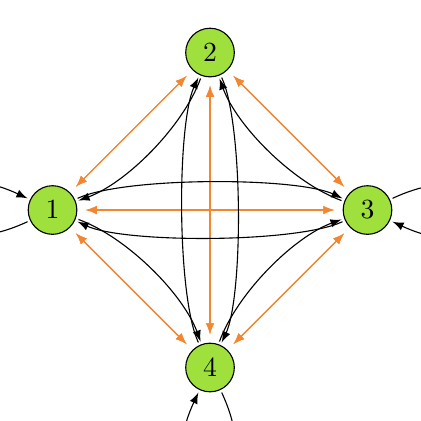
\begin{tikzpicture}
{ \definecolor{mycolor}{RGB}{159,224,61}
\node[hid, fill=mycolor] (1) at (180:2) {1};}
{ \definecolor{mycolor}{RGB}{159,224,61}
\node[hid, fill=mycolor] (2) at (90:2) {2};}
{ \definecolor{mycolor}{RGB}{159,224,61}
\node[hid, fill=mycolor] (3) at (0:2) {3};}
{ \definecolor{mycolor}{RGB}{159,224,61}
\node[hid, fill=mycolor] (4) at (-90:2) {4};}
\path[overlay,draw,pil] (1) .. controls +(205.00000:20.00000mm) and +(155.00000:20.00000mm) .. (1);
  \draw[pilip, on layer=back] (1) -- (3);
\path[overlay,draw,pil] (1) .. controls +(25.00000:10.00000mm) and +(155.00000:10.00000mm) .. (3);
  \draw[pilip, on layer=back] (1) -- (2);
  \draw[pilip, on layer=back] (1) -- (4);
\path[overlay,draw,pil] (1) .. controls +(-20.00000:10.00000mm) and +(110.00000:10.00000mm) .. (4);
  \draw[pilip, on layer=back] (2) -- (1);
\path[overlay,draw,pil] (2) .. controls +(-110.00000:10.00000mm) and +(20.00000:10.00000mm) .. (1);
  \draw[pilip, on layer=back] (2) -- (3);
  \draw[pilip, on layer=back] (2) -- (4);
\path[overlay,draw,pil] (2) .. controls +(-65.00000:10.00000mm) and +(65.00000:10.00000mm) .. (4);
  \draw[pilip, on layer=back] (3) -- (1);
\path[overlay,draw,pil] (3) .. controls +(205.00000:10.00000mm) and +(-25.00000:10.00000mm) .. (1);
\path[overlay,draw,pil] (3) .. controls +(25.00000:20.00000mm) and +(-25.00000:20.00000mm) .. (3);
  \draw[pilip, on layer=back] (3) -- (2);
\path[overlay,draw,pil] (3) .. controls +(160.00000:10.00000mm) and +(-70.00000:10.00000mm) .. (2);
  \draw[pilip, on layer=back] (3) -- (4);
  \draw[pilip, on layer=back] (4) -- (1);
  \draw[pilip, on layer=back] (4) -- (3);
\path[overlay,draw,pil] (4) .. controls +(70.00000:10.00000mm) and +(-160.00000:10.00000mm) .. (3);
  \draw[pilip, on layer=back] (4) -- (2);
\path[overlay,draw,pil] (4) .. controls +(115.00000:10.00000mm) and +(-115.00000:10.00000mm) .. (2);
\path[overlay,draw,pil] (4) .. controls +(-65.00000:20.00000mm) and +(-115.00000:20.00000mm) .. (4);

\end{tikzpicture}
};
\\
  \node[scale=0.7](){
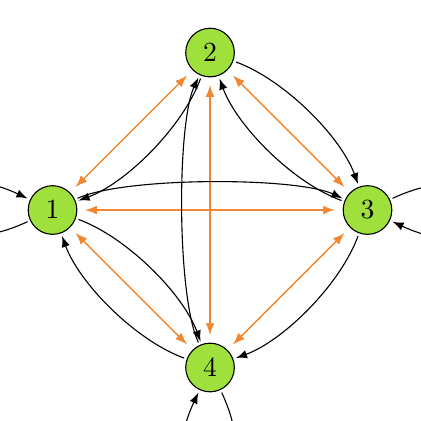
\begin{tikzpicture}
{ \definecolor{mycolor}{RGB}{159,224,61}
\node[hid, fill=mycolor] (1) at (180:2) {1};}
{ \definecolor{mycolor}{RGB}{159,224,61}
\node[hid, fill=mycolor] (2) at (90:2) {2};}
{ \definecolor{mycolor}{RGB}{159,224,61}
\node[hid, fill=mycolor] (3) at (0:2) {3};}
{ \definecolor{mycolor}{RGB}{159,224,61}
\node[hid, fill=mycolor] (4) at (-90:2) {4};}
\path[overlay,draw,pil] (1) .. controls +(205.00000:20.00000mm) and +(155.00000:20.00000mm) .. (1);
  \draw[pilip, on layer=back] (1) -- (3);
\path[overlay,draw,pil] (1) .. controls +(25.00000:10.00000mm) and +(155.00000:10.00000mm) .. (3);
  \draw[pilip, on layer=back] (1) -- (2);
  \draw[pilip, on layer=back] (1) -- (4);
\path[overlay,draw,pil] (1) .. controls +(-20.00000:10.00000mm) and +(110.00000:10.00000mm) .. (4);
  \draw[pilip, on layer=back] (2) -- (1);
\path[overlay,draw,pil] (2) .. controls +(-110.00000:10.00000mm) and +(20.00000:10.00000mm) .. (1);
  \draw[pilip, on layer=back] (2) -- (3);
\path[overlay,draw,pil] (2) .. controls +(-20.00000:10.00000mm) and +(110.00000:10.00000mm) .. (3);
  \draw[pilip, on layer=back] (2) -- (4);
  \draw[pilip, on layer=back] (3) -- (1);
\path[overlay,draw,pil] (3) .. controls +(25.00000:20.00000mm) and +(-25.00000:20.00000mm) .. (3);
  \draw[pilip, on layer=back] (3) -- (2);
\path[overlay,draw,pil] (3) .. controls +(160.00000:10.00000mm) and +(-70.00000:10.00000mm) .. (2);
  \draw[pilip, on layer=back] (3) -- (4);
\path[overlay,draw,pil] (3) .. controls +(-110.00000:10.00000mm) and +(20.00000:10.00000mm) .. (4);
  \draw[pilip, on layer=back] (4) -- (1);
\path[overlay,draw,pil] (4) .. controls +(160.00000:10.00000mm) and +(-70.00000:10.00000mm) .. (1);
  \draw[pilip, on layer=back] (4) -- (3);
  \draw[pilip, on layer=back] (4) -- (2);
\path[overlay,draw,pil] (4) .. controls +(115.00000:10.00000mm) and +(-115.00000:10.00000mm) .. (2);
\path[overlay,draw,pil] (4) .. controls +(-65.00000:20.00000mm) and +(-115.00000:20.00000mm) .. (4);

\end{tikzpicture}
};
& \node[scale=0.7](){
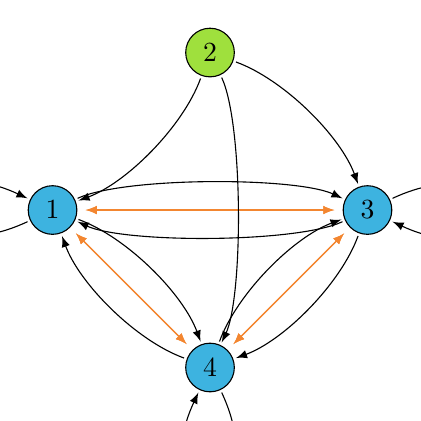
\begin{tikzpicture}
{ \definecolor{mycolor}{RGB}{61,179,224}
\node[hid, fill=mycolor] (1) at (180:2) {1};}
{ \definecolor{mycolor}{RGB}{159,224,61}
\node[hid, fill=mycolor] (2) at (90:2) {2};}
{ \definecolor{mycolor}{RGB}{61,179,224}
\node[hid, fill=mycolor] (3) at (0:2) {3};}
{ \definecolor{mycolor}{RGB}{61,179,224}
\node[hid, fill=mycolor] (4) at (-90:2) {4};}
\path[overlay,draw,pil] (1) .. controls +(205.00000:20.00000mm) and +(155.00000:20.00000mm) .. (1);
  \draw[pilip, on layer=back] (1) -- (3);
\path[overlay,draw,pil] (1) .. controls +(25.00000:10.00000mm) and +(155.00000:10.00000mm) .. (3);
  \draw[pilip, on layer=back] (1) -- (4);
\path[overlay,draw,pil] (1) .. controls +(-20.00000:10.00000mm) and +(110.00000:10.00000mm) .. (4);
\path[overlay,draw,pil] (2) .. controls +(-110.00000:10.00000mm) and +(20.00000:10.00000mm) .. (1);
\path[overlay,draw,pil] (2) .. controls +(-20.00000:10.00000mm) and +(110.00000:10.00000mm) .. (3);
\path[overlay,draw,pil] (2) .. controls +(-65.00000:10.00000mm) and +(65.00000:10.00000mm) .. (4);
  \draw[pilip, on layer=back] (3) -- (1);
\path[overlay,draw,pil] (3) .. controls +(205.00000:10.00000mm) and +(-25.00000:10.00000mm) .. (1);
\path[overlay,draw,pil] (3) .. controls +(25.00000:20.00000mm) and +(-25.00000:20.00000mm) .. (3);
  \draw[pilip, on layer=back] (3) -- (4);
\path[overlay,draw,pil] (3) .. controls +(-110.00000:10.00000mm) and +(20.00000:10.00000mm) .. (4);
  \draw[pilip, on layer=back] (4) -- (1);
\path[overlay,draw,pil] (4) .. controls +(160.00000:10.00000mm) and +(-70.00000:10.00000mm) .. (1);
  \draw[pilip, on layer=back] (4) -- (3);
\path[overlay,draw,pil] (4) .. controls +(70.00000:10.00000mm) and +(-160.00000:10.00000mm) .. (3);
\path[overlay,draw,pil] (4) .. controls +(-65.00000:20.00000mm) and +(-115.00000:20.00000mm) .. (4);

\end{tikzpicture}
};
& \node[scale=0.7](){
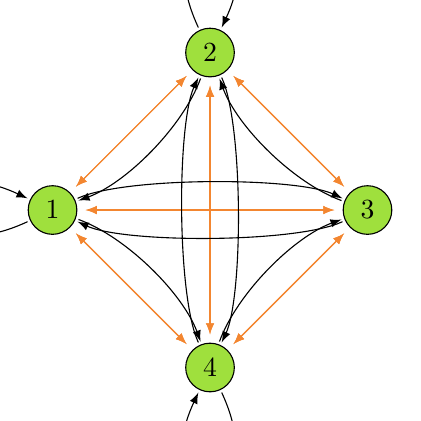
\begin{tikzpicture}
{ \definecolor{mycolor}{RGB}{159,224,61}
\node[hid, fill=mycolor] (1) at (180:2) {1};}
{ \definecolor{mycolor}{RGB}{159,224,61}
\node[hid, fill=mycolor] (2) at (90:2) {2};}
{ \definecolor{mycolor}{RGB}{159,224,61}
\node[hid, fill=mycolor] (3) at (0:2) {3};}
{ \definecolor{mycolor}{RGB}{159,224,61}
\node[hid, fill=mycolor] (4) at (-90:2) {4};}
\path[overlay,draw,pil] (1) .. controls +(205.00000:20.00000mm) and +(155.00000:20.00000mm) .. (1);
  \draw[pilip, on layer=back] (1) -- (3);
\path[overlay,draw,pil] (1) .. controls +(25.00000:10.00000mm) and +(155.00000:10.00000mm) .. (3);
  \draw[pilip, on layer=back] (1) -- (2);
  \draw[pilip, on layer=back] (1) -- (4);
\path[overlay,draw,pil] (1) .. controls +(-20.00000:10.00000mm) and +(110.00000:10.00000mm) .. (4);
  \draw[pilip, on layer=back] (2) -- (1);
\path[overlay,draw,pil] (2) .. controls +(-110.00000:10.00000mm) and +(20.00000:10.00000mm) .. (1);
  \draw[pilip, on layer=back] (2) -- (3);
\path[overlay,draw,pil] (2) .. controls +(115.00000:20.00000mm) and +(65.00000:20.00000mm) .. (2);
  \draw[pilip, on layer=back] (2) -- (4);
\path[overlay,draw,pil] (2) .. controls +(-65.00000:10.00000mm) and +(65.00000:10.00000mm) .. (4);
  \draw[pilip, on layer=back] (3) -- (1);
\path[overlay,draw,pil] (3) .. controls +(205.00000:10.00000mm) and +(-25.00000:10.00000mm) .. (1);
  \draw[pilip, on layer=back] (3) -- (2);
\path[overlay,draw,pil] (3) .. controls +(160.00000:10.00000mm) and +(-70.00000:10.00000mm) .. (2);
  \draw[pilip, on layer=back] (3) -- (4);
  \draw[pilip, on layer=back] (4) -- (1);
  \draw[pilip, on layer=back] (4) -- (3);
\path[overlay,draw,pil] (4) .. controls +(70.00000:10.00000mm) and +(-160.00000:10.00000mm) .. (3);
  \draw[pilip, on layer=back] (4) -- (2);
\path[overlay,draw,pil] (4) .. controls +(115.00000:10.00000mm) and +(-115.00000:10.00000mm) .. (2);
\path[overlay,draw,pil] (4) .. controls +(-65.00000:20.00000mm) and +(-115.00000:20.00000mm) .. (4);

\end{tikzpicture}
};
& \node[scale=0.7](){
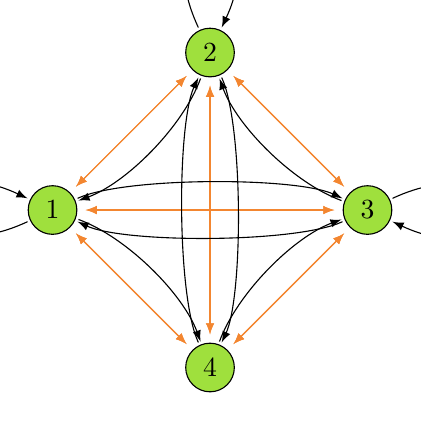
\begin{tikzpicture}
{ \definecolor{mycolor}{RGB}{159,224,61}
\node[hid, fill=mycolor] (1) at (180:2) {1};}
{ \definecolor{mycolor}{RGB}{159,224,61}
\node[hid, fill=mycolor] (2) at (90:2) {2};}
{ \definecolor{mycolor}{RGB}{159,224,61}
\node[hid, fill=mycolor] (3) at (0:2) {3};}
{ \definecolor{mycolor}{RGB}{159,224,61}
\node[hid, fill=mycolor] (4) at (-90:2) {4};}
\path[overlay,draw,pil] (1) .. controls +(205.00000:20.00000mm) and +(155.00000:20.00000mm) .. (1);
  \draw[pilip, on layer=back] (1) -- (3);
\path[overlay,draw,pil] (1) .. controls +(25.00000:10.00000mm) and +(155.00000:10.00000mm) .. (3);
  \draw[pilip, on layer=back] (1) -- (2);
  \draw[pilip, on layer=back] (1) -- (4);
\path[overlay,draw,pil] (1) .. controls +(-20.00000:10.00000mm) and +(110.00000:10.00000mm) .. (4);
  \draw[pilip, on layer=back] (2) -- (1);
\path[overlay,draw,pil] (2) .. controls +(-110.00000:10.00000mm) and +(20.00000:10.00000mm) .. (1);
  \draw[pilip, on layer=back] (2) -- (3);
\path[overlay,draw,pil] (2) .. controls +(115.00000:20.00000mm) and +(65.00000:20.00000mm) .. (2);
  \draw[pilip, on layer=back] (2) -- (4);
\path[overlay,draw,pil] (2) .. controls +(-65.00000:10.00000mm) and +(65.00000:10.00000mm) .. (4);
  \draw[pilip, on layer=back] (3) -- (1);
\path[overlay,draw,pil] (3) .. controls +(205.00000:10.00000mm) and +(-25.00000:10.00000mm) .. (1);
\path[overlay,draw,pil] (3) .. controls +(25.00000:20.00000mm) and +(-25.00000:20.00000mm) .. (3);
  \draw[pilip, on layer=back] (3) -- (2);
\path[overlay,draw,pil] (3) .. controls +(160.00000:10.00000mm) and +(-70.00000:10.00000mm) .. (2);
  \draw[pilip, on layer=back] (3) -- (4);
  \draw[pilip, on layer=back] (4) -- (1);
  \draw[pilip, on layer=back] (4) -- (3);
\path[overlay,draw,pil] (4) .. controls +(70.00000:10.00000mm) and +(-160.00000:10.00000mm) .. (3);
  \draw[pilip, on layer=back] (4) -- (2);
\path[overlay,draw,pil] (4) .. controls +(115.00000:10.00000mm) and +(-115.00000:10.00000mm) .. (2);

\end{tikzpicture}
};
& \node[scale=0.7](){
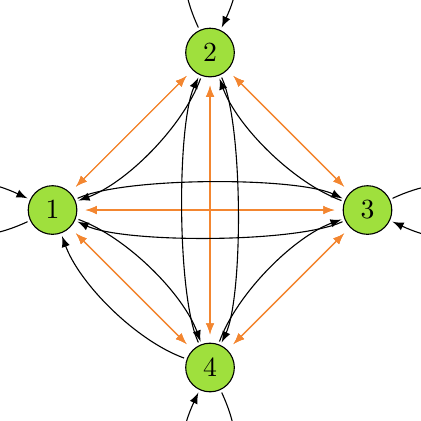
\begin{tikzpicture}
{ \definecolor{mycolor}{RGB}{159,224,61}
\node[hid, fill=mycolor] (1) at (180:2) {1};}
{ \definecolor{mycolor}{RGB}{159,224,61}
\node[hid, fill=mycolor] (2) at (90:2) {2};}
{ \definecolor{mycolor}{RGB}{159,224,61}
\node[hid, fill=mycolor] (3) at (0:2) {3};}
{ \definecolor{mycolor}{RGB}{159,224,61}
\node[hid, fill=mycolor] (4) at (-90:2) {4};}
\path[overlay,draw,pil] (1) .. controls +(205.00000:20.00000mm) and +(155.00000:20.00000mm) .. (1);
  \draw[pilip, on layer=back] (1) -- (3);
\path[overlay,draw,pil] (1) .. controls +(25.00000:10.00000mm) and +(155.00000:10.00000mm) .. (3);
  \draw[pilip, on layer=back] (1) -- (2);
  \draw[pilip, on layer=back] (1) -- (4);
\path[overlay,draw,pil] (1) .. controls +(-20.00000:10.00000mm) and +(110.00000:10.00000mm) .. (4);
  \draw[pilip, on layer=back] (2) -- (1);
\path[overlay,draw,pil] (2) .. controls +(-110.00000:10.00000mm) and +(20.00000:10.00000mm) .. (1);
  \draw[pilip, on layer=back] (2) -- (3);
\path[overlay,draw,pil] (2) .. controls +(115.00000:20.00000mm) and +(65.00000:20.00000mm) .. (2);
  \draw[pilip, on layer=back] (2) -- (4);
\path[overlay,draw,pil] (2) .. controls +(-65.00000:10.00000mm) and +(65.00000:10.00000mm) .. (4);
  \draw[pilip, on layer=back] (3) -- (1);
\path[overlay,draw,pil] (3) .. controls +(205.00000:10.00000mm) and +(-25.00000:10.00000mm) .. (1);
\path[overlay,draw,pil] (3) .. controls +(25.00000:20.00000mm) and +(-25.00000:20.00000mm) .. (3);
  \draw[pilip, on layer=back] (3) -- (2);
\path[overlay,draw,pil] (3) .. controls +(160.00000:10.00000mm) and +(-70.00000:10.00000mm) .. (2);
  \draw[pilip, on layer=back] (3) -- (4);
  \draw[pilip, on layer=back] (4) -- (1);
\path[overlay,draw,pil] (4) .. controls +(160.00000:10.00000mm) and +(-70.00000:10.00000mm) .. (1);
  \draw[pilip, on layer=back] (4) -- (3);
\path[overlay,draw,pil] (4) .. controls +(70.00000:10.00000mm) and +(-160.00000:10.00000mm) .. (3);
  \draw[pilip, on layer=back] (4) -- (2);
\path[overlay,draw,pil] (4) .. controls +(115.00000:10.00000mm) and +(-115.00000:10.00000mm) .. (2);
\path[overlay,draw,pil] (4) .. controls +(-65.00000:20.00000mm) and +(-115.00000:20.00000mm) .. (4);

\end{tikzpicture}
};
\\
  \node[scale=0.7](){
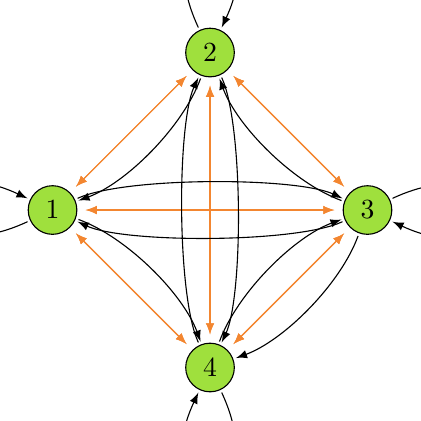
\begin{tikzpicture}
{ \definecolor{mycolor}{RGB}{159,224,61}
\node[hid, fill=mycolor] (1) at (180:2) {1};}
{ \definecolor{mycolor}{RGB}{159,224,61}
\node[hid, fill=mycolor] (2) at (90:2) {2};}
{ \definecolor{mycolor}{RGB}{159,224,61}
\node[hid, fill=mycolor] (3) at (0:2) {3};}
{ \definecolor{mycolor}{RGB}{159,224,61}
\node[hid, fill=mycolor] (4) at (-90:2) {4};}
\path[overlay,draw,pil] (1) .. controls +(205.00000:20.00000mm) and +(155.00000:20.00000mm) .. (1);
  \draw[pilip, on layer=back] (1) -- (3);
\path[overlay,draw,pil] (1) .. controls +(25.00000:10.00000mm) and +(155.00000:10.00000mm) .. (3);
  \draw[pilip, on layer=back] (1) -- (2);
  \draw[pilip, on layer=back] (1) -- (4);
\path[overlay,draw,pil] (1) .. controls +(-20.00000:10.00000mm) and +(110.00000:10.00000mm) .. (4);
  \draw[pilip, on layer=back] (2) -- (1);
\path[overlay,draw,pil] (2) .. controls +(-110.00000:10.00000mm) and +(20.00000:10.00000mm) .. (1);
  \draw[pilip, on layer=back] (2) -- (3);
\path[overlay,draw,pil] (2) .. controls +(115.00000:20.00000mm) and +(65.00000:20.00000mm) .. (2);
  \draw[pilip, on layer=back] (2) -- (4);
\path[overlay,draw,pil] (2) .. controls +(-65.00000:10.00000mm) and +(65.00000:10.00000mm) .. (4);
  \draw[pilip, on layer=back] (3) -- (1);
\path[overlay,draw,pil] (3) .. controls +(205.00000:10.00000mm) and +(-25.00000:10.00000mm) .. (1);
\path[overlay,draw,pil] (3) .. controls +(25.00000:20.00000mm) and +(-25.00000:20.00000mm) .. (3);
  \draw[pilip, on layer=back] (3) -- (2);
\path[overlay,draw,pil] (3) .. controls +(160.00000:10.00000mm) and +(-70.00000:10.00000mm) .. (2);
  \draw[pilip, on layer=back] (3) -- (4);
\path[overlay,draw,pil] (3) .. controls +(-110.00000:10.00000mm) and +(20.00000:10.00000mm) .. (4);
  \draw[pilip, on layer=back] (4) -- (1);
  \draw[pilip, on layer=back] (4) -- (3);
\path[overlay,draw,pil] (4) .. controls +(70.00000:10.00000mm) and +(-160.00000:10.00000mm) .. (3);
  \draw[pilip, on layer=back] (4) -- (2);
\path[overlay,draw,pil] (4) .. controls +(115.00000:10.00000mm) and +(-115.00000:10.00000mm) .. (2);
\path[overlay,draw,pil] (4) .. controls +(-65.00000:20.00000mm) and +(-115.00000:20.00000mm) .. (4);

\end{tikzpicture}
};
& \node[scale=0.7](){
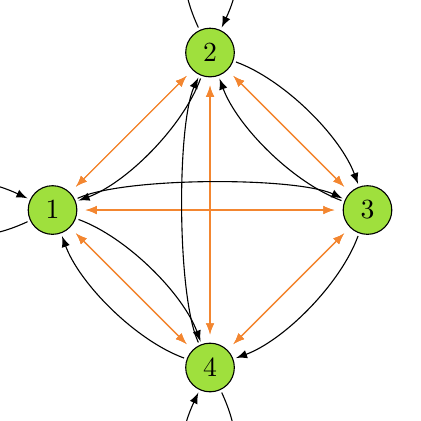
\begin{tikzpicture}
{ \definecolor{mycolor}{RGB}{159,224,61}
\node[hid, fill=mycolor] (1) at (180:2) {1};}
{ \definecolor{mycolor}{RGB}{159,224,61}
\node[hid, fill=mycolor] (2) at (90:2) {2};}
{ \definecolor{mycolor}{RGB}{159,224,61}
\node[hid, fill=mycolor] (3) at (0:2) {3};}
{ \definecolor{mycolor}{RGB}{159,224,61}
\node[hid, fill=mycolor] (4) at (-90:2) {4};}
\path[overlay,draw,pil] (1) .. controls +(205.00000:20.00000mm) and +(155.00000:20.00000mm) .. (1);
  \draw[pilip, on layer=back] (1) -- (3);
\path[overlay,draw,pil] (1) .. controls +(25.00000:10.00000mm) and +(155.00000:10.00000mm) .. (3);
  \draw[pilip, on layer=back] (1) -- (2);
  \draw[pilip, on layer=back] (1) -- (4);
\path[overlay,draw,pil] (1) .. controls +(-20.00000:10.00000mm) and +(110.00000:10.00000mm) .. (4);
  \draw[pilip, on layer=back] (2) -- (1);
\path[overlay,draw,pil] (2) .. controls +(-110.00000:10.00000mm) and +(20.00000:10.00000mm) .. (1);
  \draw[pilip, on layer=back] (2) -- (3);
\path[overlay,draw,pil] (2) .. controls +(-20.00000:10.00000mm) and +(110.00000:10.00000mm) .. (3);
\path[overlay,draw,pil] (2) .. controls +(115.00000:20.00000mm) and +(65.00000:20.00000mm) .. (2);
  \draw[pilip, on layer=back] (2) -- (4);
  \draw[pilip, on layer=back] (3) -- (1);
  \draw[pilip, on layer=back] (3) -- (2);
\path[overlay,draw,pil] (3) .. controls +(160.00000:10.00000mm) and +(-70.00000:10.00000mm) .. (2);
  \draw[pilip, on layer=back] (3) -- (4);
\path[overlay,draw,pil] (3) .. controls +(-110.00000:10.00000mm) and +(20.00000:10.00000mm) .. (4);
  \draw[pilip, on layer=back] (4) -- (1);
\path[overlay,draw,pil] (4) .. controls +(160.00000:10.00000mm) and +(-70.00000:10.00000mm) .. (1);
  \draw[pilip, on layer=back] (4) -- (3);
  \draw[pilip, on layer=back] (4) -- (2);
\path[overlay,draw,pil] (4) .. controls +(115.00000:10.00000mm) and +(-115.00000:10.00000mm) .. (2);
\path[overlay,draw,pil] (4) .. controls +(-65.00000:20.00000mm) and +(-115.00000:20.00000mm) .. (4);

\end{tikzpicture}
};
& \node[scale=0.7](){
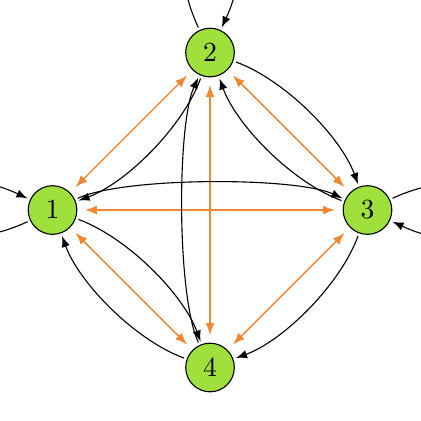
\begin{tikzpicture}
{ \definecolor{mycolor}{RGB}{159,224,61}
\node[hid, fill=mycolor] (1) at (180:2) {1};}
{ \definecolor{mycolor}{RGB}{159,224,61}
\node[hid, fill=mycolor] (2) at (90:2) {2};}
{ \definecolor{mycolor}{RGB}{159,224,61}
\node[hid, fill=mycolor] (3) at (0:2) {3};}
{ \definecolor{mycolor}{RGB}{159,224,61}
\node[hid, fill=mycolor] (4) at (-90:2) {4};}
\path[overlay,draw,pil] (1) .. controls +(205.00000:20.00000mm) and +(155.00000:20.00000mm) .. (1);
  \draw[pilip, on layer=back] (1) -- (3);
\path[overlay,draw,pil] (1) .. controls +(25.00000:10.00000mm) and +(155.00000:10.00000mm) .. (3);
  \draw[pilip, on layer=back] (1) -- (2);
  \draw[pilip, on layer=back] (1) -- (4);
\path[overlay,draw,pil] (1) .. controls +(-20.00000:10.00000mm) and +(110.00000:10.00000mm) .. (4);
  \draw[pilip, on layer=back] (2) -- (1);
\path[overlay,draw,pil] (2) .. controls +(-110.00000:10.00000mm) and +(20.00000:10.00000mm) .. (1);
  \draw[pilip, on layer=back] (2) -- (3);
\path[overlay,draw,pil] (2) .. controls +(-20.00000:10.00000mm) and +(110.00000:10.00000mm) .. (3);
\path[overlay,draw,pil] (2) .. controls +(115.00000:20.00000mm) and +(65.00000:20.00000mm) .. (2);
  \draw[pilip, on layer=back] (2) -- (4);
  \draw[pilip, on layer=back] (3) -- (1);
\path[overlay,draw,pil] (3) .. controls +(25.00000:20.00000mm) and +(-25.00000:20.00000mm) .. (3);
  \draw[pilip, on layer=back] (3) -- (2);
\path[overlay,draw,pil] (3) .. controls +(160.00000:10.00000mm) and +(-70.00000:10.00000mm) .. (2);
  \draw[pilip, on layer=back] (3) -- (4);
\path[overlay,draw,pil] (3) .. controls +(-110.00000:10.00000mm) and +(20.00000:10.00000mm) .. (4);
  \draw[pilip, on layer=back] (4) -- (1);
\path[overlay,draw,pil] (4) .. controls +(160.00000:10.00000mm) and +(-70.00000:10.00000mm) .. (1);
  \draw[pilip, on layer=back] (4) -- (3);
  \draw[pilip, on layer=back] (4) -- (2);
\path[overlay,draw,pil] (4) .. controls +(115.00000:10.00000mm) and +(-115.00000:10.00000mm) .. (2);

\end{tikzpicture}
};
& \node[scale=0.7](){
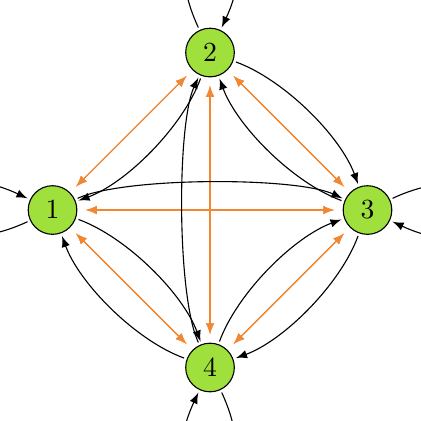
\begin{tikzpicture}
{ \definecolor{mycolor}{RGB}{159,224,61}
\node[hid, fill=mycolor] (1) at (180:2) {1};}
{ \definecolor{mycolor}{RGB}{159,224,61}
\node[hid, fill=mycolor] (2) at (90:2) {2};}
{ \definecolor{mycolor}{RGB}{159,224,61}
\node[hid, fill=mycolor] (3) at (0:2) {3};}
{ \definecolor{mycolor}{RGB}{159,224,61}
\node[hid, fill=mycolor] (4) at (-90:2) {4};}
\path[overlay,draw,pil] (1) .. controls +(205.00000:20.00000mm) and +(155.00000:20.00000mm) .. (1);
  \draw[pilip, on layer=back] (1) -- (3);
\path[overlay,draw,pil] (1) .. controls +(25.00000:10.00000mm) and +(155.00000:10.00000mm) .. (3);
  \draw[pilip, on layer=back] (1) -- (2);
  \draw[pilip, on layer=back] (1) -- (4);
\path[overlay,draw,pil] (1) .. controls +(-20.00000:10.00000mm) and +(110.00000:10.00000mm) .. (4);
  \draw[pilip, on layer=back] (2) -- (1);
\path[overlay,draw,pil] (2) .. controls +(-110.00000:10.00000mm) and +(20.00000:10.00000mm) .. (1);
  \draw[pilip, on layer=back] (2) -- (3);
\path[overlay,draw,pil] (2) .. controls +(-20.00000:10.00000mm) and +(110.00000:10.00000mm) .. (3);
\path[overlay,draw,pil] (2) .. controls +(115.00000:20.00000mm) and +(65.00000:20.00000mm) .. (2);
  \draw[pilip, on layer=back] (2) -- (4);
  \draw[pilip, on layer=back] (3) -- (1);
\path[overlay,draw,pil] (3) .. controls +(25.00000:20.00000mm) and +(-25.00000:20.00000mm) .. (3);
  \draw[pilip, on layer=back] (3) -- (2);
\path[overlay,draw,pil] (3) .. controls +(160.00000:10.00000mm) and +(-70.00000:10.00000mm) .. (2);
  \draw[pilip, on layer=back] (3) -- (4);
\path[overlay,draw,pil] (3) .. controls +(-110.00000:10.00000mm) and +(20.00000:10.00000mm) .. (4);
  \draw[pilip, on layer=back] (4) -- (1);
\path[overlay,draw,pil] (4) .. controls +(160.00000:10.00000mm) and +(-70.00000:10.00000mm) .. (1);
  \draw[pilip, on layer=back] (4) -- (3);
\path[overlay,draw,pil] (4) .. controls +(70.00000:10.00000mm) and +(-160.00000:10.00000mm) .. (3);
  \draw[pilip, on layer=back] (4) -- (2);
\path[overlay,draw,pil] (4) .. controls +(115.00000:10.00000mm) and +(-115.00000:10.00000mm) .. (2);
\path[overlay,draw,pil] (4) .. controls +(-65.00000:20.00000mm) and +(-115.00000:20.00000mm) .. (4);

\end{tikzpicture}
};
& \node[scale=0.7](){
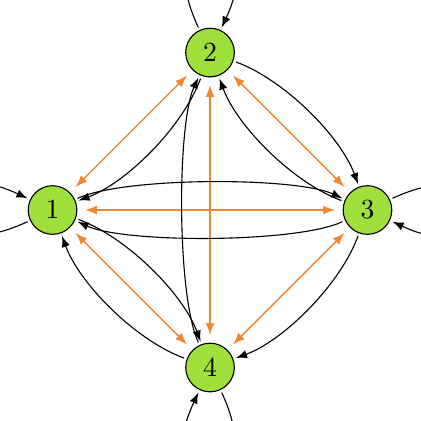
\begin{tikzpicture}
{ \definecolor{mycolor}{RGB}{159,224,61}
\node[hid, fill=mycolor] (1) at (180:2) {1};}
{ \definecolor{mycolor}{RGB}{159,224,61}
\node[hid, fill=mycolor] (2) at (90:2) {2};}
{ \definecolor{mycolor}{RGB}{159,224,61}
\node[hid, fill=mycolor] (3) at (0:2) {3};}
{ \definecolor{mycolor}{RGB}{159,224,61}
\node[hid, fill=mycolor] (4) at (-90:2) {4};}
\path[overlay,draw,pil] (1) .. controls +(205.00000:20.00000mm) and +(155.00000:20.00000mm) .. (1);
  \draw[pilip, on layer=back] (1) -- (3);
\path[overlay,draw,pil] (1) .. controls +(25.00000:10.00000mm) and +(155.00000:10.00000mm) .. (3);
  \draw[pilip, on layer=back] (1) -- (2);
  \draw[pilip, on layer=back] (1) -- (4);
\path[overlay,draw,pil] (1) .. controls +(-20.00000:10.00000mm) and +(110.00000:10.00000mm) .. (4);
  \draw[pilip, on layer=back] (2) -- (1);
\path[overlay,draw,pil] (2) .. controls +(-110.00000:10.00000mm) and +(20.00000:10.00000mm) .. (1);
  \draw[pilip, on layer=back] (2) -- (3);
\path[overlay,draw,pil] (2) .. controls +(-20.00000:10.00000mm) and +(110.00000:10.00000mm) .. (3);
\path[overlay,draw,pil] (2) .. controls +(115.00000:20.00000mm) and +(65.00000:20.00000mm) .. (2);
  \draw[pilip, on layer=back] (2) -- (4);
  \draw[pilip, on layer=back] (3) -- (1);
\path[overlay,draw,pil] (3) .. controls +(205.00000:10.00000mm) and +(-25.00000:10.00000mm) .. (1);
\path[overlay,draw,pil] (3) .. controls +(25.00000:20.00000mm) and +(-25.00000:20.00000mm) .. (3);
  \draw[pilip, on layer=back] (3) -- (2);
\path[overlay,draw,pil] (3) .. controls +(160.00000:10.00000mm) and +(-70.00000:10.00000mm) .. (2);
  \draw[pilip, on layer=back] (3) -- (4);
\path[overlay,draw,pil] (3) .. controls +(-110.00000:10.00000mm) and +(20.00000:10.00000mm) .. (4);
  \draw[pilip, on layer=back] (4) -- (1);
\path[overlay,draw,pil] (4) .. controls +(160.00000:10.00000mm) and +(-70.00000:10.00000mm) .. (1);
  \draw[pilip, on layer=back] (4) -- (3);
  \draw[pilip, on layer=back] (4) -- (2);
\path[overlay,draw,pil] (4) .. controls +(115.00000:10.00000mm) and +(-115.00000:10.00000mm) .. (2);
\path[overlay,draw,pil] (4) .. controls +(-65.00000:20.00000mm) and +(-115.00000:20.00000mm) .. (4);

\end{tikzpicture}
};
\\
  \node[scale=0.7](){
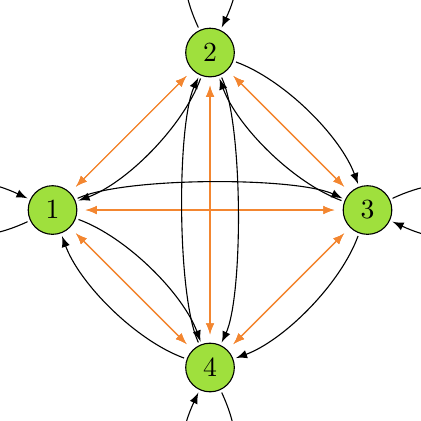
\begin{tikzpicture}
{ \definecolor{mycolor}{RGB}{159,224,61}
\node[hid, fill=mycolor] (1) at (180:2) {1};}
{ \definecolor{mycolor}{RGB}{159,224,61}
\node[hid, fill=mycolor] (2) at (90:2) {2};}
{ \definecolor{mycolor}{RGB}{159,224,61}
\node[hid, fill=mycolor] (3) at (0:2) {3};}
{ \definecolor{mycolor}{RGB}{159,224,61}
\node[hid, fill=mycolor] (4) at (-90:2) {4};}
\path[overlay,draw,pil] (1) .. controls +(205.00000:20.00000mm) and +(155.00000:20.00000mm) .. (1);
  \draw[pilip, on layer=back] (1) -- (3);
\path[overlay,draw,pil] (1) .. controls +(25.00000:10.00000mm) and +(155.00000:10.00000mm) .. (3);
  \draw[pilip, on layer=back] (1) -- (2);
  \draw[pilip, on layer=back] (1) -- (4);
\path[overlay,draw,pil] (1) .. controls +(-20.00000:10.00000mm) and +(110.00000:10.00000mm) .. (4);
  \draw[pilip, on layer=back] (2) -- (1);
\path[overlay,draw,pil] (2) .. controls +(-110.00000:10.00000mm) and +(20.00000:10.00000mm) .. (1);
  \draw[pilip, on layer=back] (2) -- (3);
\path[overlay,draw,pil] (2) .. controls +(-20.00000:10.00000mm) and +(110.00000:10.00000mm) .. (3);
\path[overlay,draw,pil] (2) .. controls +(115.00000:20.00000mm) and +(65.00000:20.00000mm) .. (2);
  \draw[pilip, on layer=back] (2) -- (4);
\path[overlay,draw,pil] (2) .. controls +(-65.00000:10.00000mm) and +(65.00000:10.00000mm) .. (4);
  \draw[pilip, on layer=back] (3) -- (1);
\path[overlay,draw,pil] (3) .. controls +(25.00000:20.00000mm) and +(-25.00000:20.00000mm) .. (3);
  \draw[pilip, on layer=back] (3) -- (2);
\path[overlay,draw,pil] (3) .. controls +(160.00000:10.00000mm) and +(-70.00000:10.00000mm) .. (2);
  \draw[pilip, on layer=back] (3) -- (4);
\path[overlay,draw,pil] (3) .. controls +(-110.00000:10.00000mm) and +(20.00000:10.00000mm) .. (4);
  \draw[pilip, on layer=back] (4) -- (1);
\path[overlay,draw,pil] (4) .. controls +(160.00000:10.00000mm) and +(-70.00000:10.00000mm) .. (1);
  \draw[pilip, on layer=back] (4) -- (3);
  \draw[pilip, on layer=back] (4) -- (2);
\path[overlay,draw,pil] (4) .. controls +(115.00000:10.00000mm) and +(-115.00000:10.00000mm) .. (2);
\path[overlay,draw,pil] (4) .. controls +(-65.00000:20.00000mm) and +(-115.00000:20.00000mm) .. (4);

\end{tikzpicture}
};
& \node[scale=0.7](){
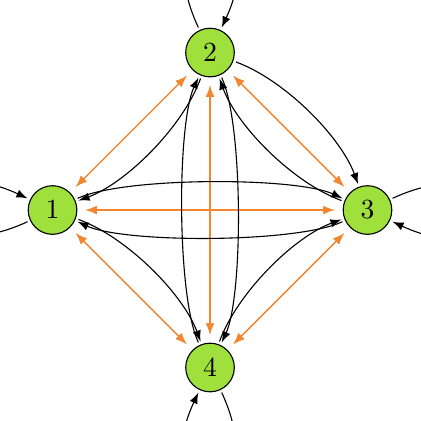
\begin{tikzpicture}
{ \definecolor{mycolor}{RGB}{159,224,61}
\node[hid, fill=mycolor] (1) at (180:2) {1};}
{ \definecolor{mycolor}{RGB}{159,224,61}
\node[hid, fill=mycolor] (2) at (90:2) {2};}
{ \definecolor{mycolor}{RGB}{159,224,61}
\node[hid, fill=mycolor] (3) at (0:2) {3};}
{ \definecolor{mycolor}{RGB}{159,224,61}
\node[hid, fill=mycolor] (4) at (-90:2) {4};}
\path[overlay,draw,pil] (1) .. controls +(205.00000:20.00000mm) and +(155.00000:20.00000mm) .. (1);
  \draw[pilip, on layer=back] (1) -- (3);
\path[overlay,draw,pil] (1) .. controls +(25.00000:10.00000mm) and +(155.00000:10.00000mm) .. (3);
  \draw[pilip, on layer=back] (1) -- (2);
  \draw[pilip, on layer=back] (1) -- (4);
\path[overlay,draw,pil] (1) .. controls +(-20.00000:10.00000mm) and +(110.00000:10.00000mm) .. (4);
  \draw[pilip, on layer=back] (2) -- (1);
\path[overlay,draw,pil] (2) .. controls +(-110.00000:10.00000mm) and +(20.00000:10.00000mm) .. (1);
  \draw[pilip, on layer=back] (2) -- (3);
\path[overlay,draw,pil] (2) .. controls +(-20.00000:10.00000mm) and +(110.00000:10.00000mm) .. (3);
\path[overlay,draw,pil] (2) .. controls +(115.00000:20.00000mm) and +(65.00000:20.00000mm) .. (2);
  \draw[pilip, on layer=back] (2) -- (4);
\path[overlay,draw,pil] (2) .. controls +(-65.00000:10.00000mm) and +(65.00000:10.00000mm) .. (4);
  \draw[pilip, on layer=back] (3) -- (1);
\path[overlay,draw,pil] (3) .. controls +(205.00000:10.00000mm) and +(-25.00000:10.00000mm) .. (1);
\path[overlay,draw,pil] (3) .. controls +(25.00000:20.00000mm) and +(-25.00000:20.00000mm) .. (3);
  \draw[pilip, on layer=back] (3) -- (2);
\path[overlay,draw,pil] (3) .. controls +(160.00000:10.00000mm) and +(-70.00000:10.00000mm) .. (2);
  \draw[pilip, on layer=back] (3) -- (4);
  \draw[pilip, on layer=back] (4) -- (1);
  \draw[pilip, on layer=back] (4) -- (3);
\path[overlay,draw,pil] (4) .. controls +(70.00000:10.00000mm) and +(-160.00000:10.00000mm) .. (3);
  \draw[pilip, on layer=back] (4) -- (2);
\path[overlay,draw,pil] (4) .. controls +(115.00000:10.00000mm) and +(-115.00000:10.00000mm) .. (2);
\path[overlay,draw,pil] (4) .. controls +(-65.00000:20.00000mm) and +(-115.00000:20.00000mm) .. (4);

\end{tikzpicture}
};
& \node[scale=0.7](){
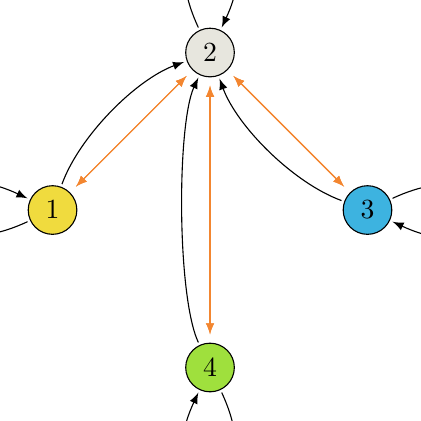
\begin{tikzpicture}
{ \definecolor{mycolor}{RGB}{240,219,62}
\node[hid, fill=mycolor] (1) at (180:2) {1};}
{ \definecolor{mycolor}{RGB}{231,230,222}
\node[hid, fill=mycolor] (2) at (90:2) {2};}
{ \definecolor{mycolor}{RGB}{61,179,224}
\node[hid, fill=mycolor] (3) at (0:2) {3};}
{ \definecolor{mycolor}{RGB}{159,224,61}
\node[hid, fill=mycolor] (4) at (-90:2) {4};}
\path[overlay,draw,pil] (1) .. controls +(205.00000:20.00000mm) and +(155.00000:20.00000mm) .. (1);
  \draw[pilip, on layer=back] (1) -- (2);
\path[overlay,draw,pil] (1) .. controls +(70.00000:10.00000mm) and +(-160.00000:10.00000mm) .. (2);
  \draw[pilip, on layer=back] (2) -- (1);
  \draw[pilip, on layer=back] (2) -- (3);
\path[overlay,draw,pil] (2) .. controls +(115.00000:20.00000mm) and +(65.00000:20.00000mm) .. (2);
  \draw[pilip, on layer=back] (2) -- (4);
\path[overlay,draw,pil] (3) .. controls +(25.00000:20.00000mm) and +(-25.00000:20.00000mm) .. (3);
  \draw[pilip, on layer=back] (3) -- (2);
\path[overlay,draw,pil] (3) .. controls +(160.00000:10.00000mm) and +(-70.00000:10.00000mm) .. (2);
  \draw[pilip, on layer=back] (4) -- (2);
\path[overlay,draw,pil] (4) .. controls +(115.00000:10.00000mm) and +(-115.00000:10.00000mm) .. (2);
\path[overlay,draw,pil] (4) .. controls +(-65.00000:20.00000mm) and +(-115.00000:20.00000mm) .. (4);

\end{tikzpicture}
};
& \node[scale=0.7](){
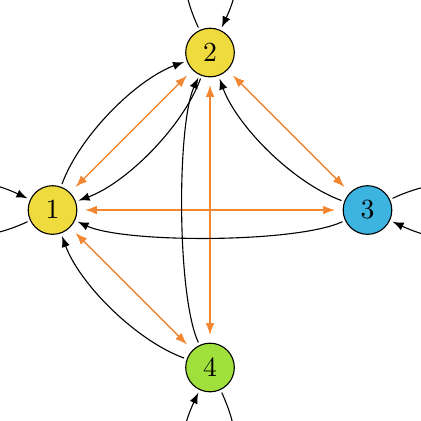
\begin{tikzpicture}
{ \definecolor{mycolor}{RGB}{240,219,62}
\node[hid, fill=mycolor] (1) at (180:2) {1};}
{ \definecolor{mycolor}{RGB}{240,219,62}
\node[hid, fill=mycolor] (2) at (90:2) {2};}
{ \definecolor{mycolor}{RGB}{61,179,224}
\node[hid, fill=mycolor] (3) at (0:2) {3};}
{ \definecolor{mycolor}{RGB}{159,224,61}
\node[hid, fill=mycolor] (4) at (-90:2) {4};}
\path[overlay,draw,pil] (1) .. controls +(205.00000:20.00000mm) and +(155.00000:20.00000mm) .. (1);
  \draw[pilip, on layer=back] (1) -- (3);
  \draw[pilip, on layer=back] (1) -- (2);
\path[overlay,draw,pil] (1) .. controls +(70.00000:10.00000mm) and +(-160.00000:10.00000mm) .. (2);
  \draw[pilip, on layer=back] (1) -- (4);
  \draw[pilip, on layer=back] (2) -- (1);
\path[overlay,draw,pil] (2) .. controls +(-110.00000:10.00000mm) and +(20.00000:10.00000mm) .. (1);
  \draw[pilip, on layer=back] (2) -- (3);
\path[overlay,draw,pil] (2) .. controls +(115.00000:20.00000mm) and +(65.00000:20.00000mm) .. (2);
  \draw[pilip, on layer=back] (2) -- (4);
  \draw[pilip, on layer=back] (3) -- (1);
\path[overlay,draw,pil] (3) .. controls +(205.00000:10.00000mm) and +(-25.00000:10.00000mm) .. (1);
\path[overlay,draw,pil] (3) .. controls +(25.00000:20.00000mm) and +(-25.00000:20.00000mm) .. (3);
  \draw[pilip, on layer=back] (3) -- (2);
\path[overlay,draw,pil] (3) .. controls +(160.00000:10.00000mm) and +(-70.00000:10.00000mm) .. (2);
  \draw[pilip, on layer=back] (4) -- (1);
\path[overlay,draw,pil] (4) .. controls +(160.00000:10.00000mm) and +(-70.00000:10.00000mm) .. (1);
  \draw[pilip, on layer=back] (4) -- (2);
\path[overlay,draw,pil] (4) .. controls +(115.00000:10.00000mm) and +(-115.00000:10.00000mm) .. (2);
\path[overlay,draw,pil] (4) .. controls +(-65.00000:20.00000mm) and +(-115.00000:20.00000mm) .. (4);

\end{tikzpicture}
};
& \node[scale=0.7](){
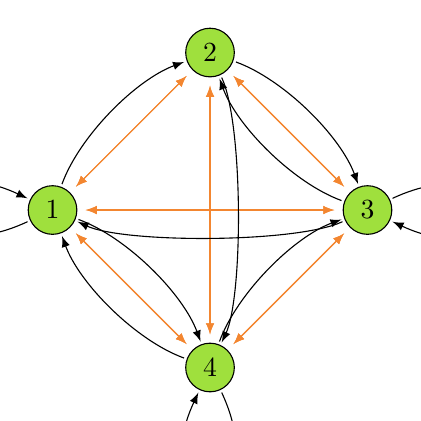
\begin{tikzpicture}
{ \definecolor{mycolor}{RGB}{159,224,61}
\node[hid, fill=mycolor] (1) at (180:2) {1};}
{ \definecolor{mycolor}{RGB}{159,224,61}
\node[hid, fill=mycolor] (2) at (90:2) {2};}
{ \definecolor{mycolor}{RGB}{159,224,61}
\node[hid, fill=mycolor] (3) at (0:2) {3};}
{ \definecolor{mycolor}{RGB}{159,224,61}
\node[hid, fill=mycolor] (4) at (-90:2) {4};}
\path[overlay,draw,pil] (1) .. controls +(205.00000:20.00000mm) and +(155.00000:20.00000mm) .. (1);
  \draw[pilip, on layer=back] (1) -- (3);
  \draw[pilip, on layer=back] (1) -- (2);
\path[overlay,draw,pil] (1) .. controls +(70.00000:10.00000mm) and +(-160.00000:10.00000mm) .. (2);
  \draw[pilip, on layer=back] (1) -- (4);
\path[overlay,draw,pil] (1) .. controls +(-20.00000:10.00000mm) and +(110.00000:10.00000mm) .. (4);
  \draw[pilip, on layer=back] (2) -- (1);
  \draw[pilip, on layer=back] (2) -- (3);
\path[overlay,draw,pil] (2) .. controls +(-20.00000:10.00000mm) and +(110.00000:10.00000mm) .. (3);
  \draw[pilip, on layer=back] (2) -- (4);
\path[overlay,draw,pil] (2) .. controls +(-65.00000:10.00000mm) and +(65.00000:10.00000mm) .. (4);
  \draw[pilip, on layer=back] (3) -- (1);
\path[overlay,draw,pil] (3) .. controls +(205.00000:10.00000mm) and +(-25.00000:10.00000mm) .. (1);
\path[overlay,draw,pil] (3) .. controls +(25.00000:20.00000mm) and +(-25.00000:20.00000mm) .. (3);
  \draw[pilip, on layer=back] (3) -- (2);
\path[overlay,draw,pil] (3) .. controls +(160.00000:10.00000mm) and +(-70.00000:10.00000mm) .. (2);
  \draw[pilip, on layer=back] (3) -- (4);
  \draw[pilip, on layer=back] (4) -- (1);
\path[overlay,draw,pil] (4) .. controls +(160.00000:10.00000mm) and +(-70.00000:10.00000mm) .. (1);
  \draw[pilip, on layer=back] (4) -- (3);
\path[overlay,draw,pil] (4) .. controls +(70.00000:10.00000mm) and +(-160.00000:10.00000mm) .. (3);
  \draw[pilip, on layer=back] (4) -- (2);
\path[overlay,draw,pil] (4) .. controls +(-65.00000:20.00000mm) and +(-115.00000:20.00000mm) .. (4);

\end{tikzpicture}
};
\\
  \node[scale=0.7](){
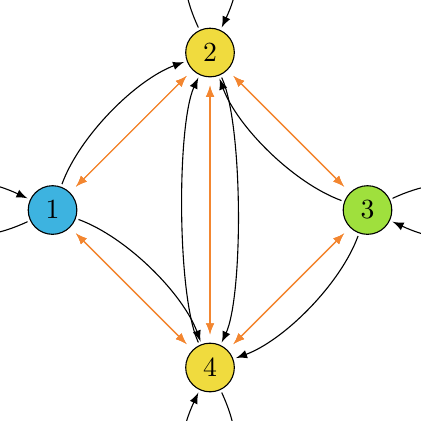
\begin{tikzpicture}
{ \definecolor{mycolor}{RGB}{61,179,224}
\node[hid, fill=mycolor] (1) at (180:2) {1};}
{ \definecolor{mycolor}{RGB}{240,219,62}
\node[hid, fill=mycolor] (2) at (90:2) {2};}
{ \definecolor{mycolor}{RGB}{159,224,61}
\node[hid, fill=mycolor] (3) at (0:2) {3};}
{ \definecolor{mycolor}{RGB}{240,219,62}
\node[hid, fill=mycolor] (4) at (-90:2) {4};}
\path[overlay,draw,pil] (1) .. controls +(205.00000:20.00000mm) and +(155.00000:20.00000mm) .. (1);
  \draw[pilip, on layer=back] (1) -- (2);
\path[overlay,draw,pil] (1) .. controls +(70.00000:10.00000mm) and +(-160.00000:10.00000mm) .. (2);
  \draw[pilip, on layer=back] (1) -- (4);
\path[overlay,draw,pil] (1) .. controls +(-20.00000:10.00000mm) and +(110.00000:10.00000mm) .. (4);
  \draw[pilip, on layer=back] (2) -- (1);
  \draw[pilip, on layer=back] (2) -- (3);
\path[overlay,draw,pil] (2) .. controls +(115.00000:20.00000mm) and +(65.00000:20.00000mm) .. (2);
  \draw[pilip, on layer=back] (2) -- (4);
\path[overlay,draw,pil] (2) .. controls +(-65.00000:10.00000mm) and +(65.00000:10.00000mm) .. (4);
\path[overlay,draw,pil] (3) .. controls +(25.00000:20.00000mm) and +(-25.00000:20.00000mm) .. (3);
  \draw[pilip, on layer=back] (3) -- (2);
\path[overlay,draw,pil] (3) .. controls +(160.00000:10.00000mm) and +(-70.00000:10.00000mm) .. (2);
  \draw[pilip, on layer=back] (3) -- (4);
\path[overlay,draw,pil] (3) .. controls +(-110.00000:10.00000mm) and +(20.00000:10.00000mm) .. (4);
  \draw[pilip, on layer=back] (4) -- (1);
  \draw[pilip, on layer=back] (4) -- (3);
  \draw[pilip, on layer=back] (4) -- (2);
\path[overlay,draw,pil] (4) .. controls +(115.00000:10.00000mm) and +(-115.00000:10.00000mm) .. (2);
\path[overlay,draw,pil] (4) .. controls +(-65.00000:20.00000mm) and +(-115.00000:20.00000mm) .. (4);

\end{tikzpicture}
};
& \node[scale=0.7](){
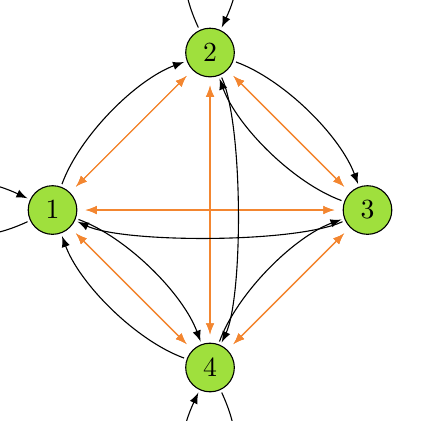
\begin{tikzpicture}
{ \definecolor{mycolor}{RGB}{159,224,61}
\node[hid, fill=mycolor] (1) at (180:2) {1};}
{ \definecolor{mycolor}{RGB}{159,224,61}
\node[hid, fill=mycolor] (2) at (90:2) {2};}
{ \definecolor{mycolor}{RGB}{159,224,61}
\node[hid, fill=mycolor] (3) at (0:2) {3};}
{ \definecolor{mycolor}{RGB}{159,224,61}
\node[hid, fill=mycolor] (4) at (-90:2) {4};}
\path[overlay,draw,pil] (1) .. controls +(205.00000:20.00000mm) and +(155.00000:20.00000mm) .. (1);
  \draw[pilip, on layer=back] (1) -- (3);
  \draw[pilip, on layer=back] (1) -- (2);
\path[overlay,draw,pil] (1) .. controls +(70.00000:10.00000mm) and +(-160.00000:10.00000mm) .. (2);
  \draw[pilip, on layer=back] (1) -- (4);
\path[overlay,draw,pil] (1) .. controls +(-20.00000:10.00000mm) and +(110.00000:10.00000mm) .. (4);
  \draw[pilip, on layer=back] (2) -- (1);
  \draw[pilip, on layer=back] (2) -- (3);
\path[overlay,draw,pil] (2) .. controls +(-20.00000:10.00000mm) and +(110.00000:10.00000mm) .. (3);
\path[overlay,draw,pil] (2) .. controls +(115.00000:20.00000mm) and +(65.00000:20.00000mm) .. (2);
  \draw[pilip, on layer=back] (2) -- (4);
\path[overlay,draw,pil] (2) .. controls +(-65.00000:10.00000mm) and +(65.00000:10.00000mm) .. (4);
  \draw[pilip, on layer=back] (3) -- (1);
\path[overlay,draw,pil] (3) .. controls +(205.00000:10.00000mm) and +(-25.00000:10.00000mm) .. (1);
  \draw[pilip, on layer=back] (3) -- (2);
\path[overlay,draw,pil] (3) .. controls +(160.00000:10.00000mm) and +(-70.00000:10.00000mm) .. (2);
  \draw[pilip, on layer=back] (3) -- (4);
  \draw[pilip, on layer=back] (4) -- (1);
\path[overlay,draw,pil] (4) .. controls +(160.00000:10.00000mm) and +(-70.00000:10.00000mm) .. (1);
  \draw[pilip, on layer=back] (4) -- (3);
\path[overlay,draw,pil] (4) .. controls +(70.00000:10.00000mm) and +(-160.00000:10.00000mm) .. (3);
  \draw[pilip, on layer=back] (4) -- (2);
\path[overlay,draw,pil] (4) .. controls +(-65.00000:20.00000mm) and +(-115.00000:20.00000mm) .. (4);

\end{tikzpicture}
};
& \node[scale=0.7](){
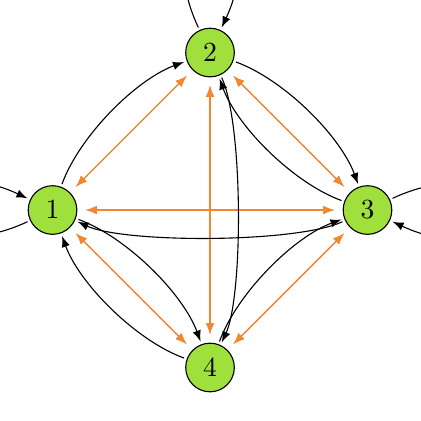
\begin{tikzpicture}
{ \definecolor{mycolor}{RGB}{159,224,61}
\node[hid, fill=mycolor] (1) at (180:2) {1};}
{ \definecolor{mycolor}{RGB}{159,224,61}
\node[hid, fill=mycolor] (2) at (90:2) {2};}
{ \definecolor{mycolor}{RGB}{159,224,61}
\node[hid, fill=mycolor] (3) at (0:2) {3};}
{ \definecolor{mycolor}{RGB}{159,224,61}
\node[hid, fill=mycolor] (4) at (-90:2) {4};}
\path[overlay,draw,pil] (1) .. controls +(205.00000:20.00000mm) and +(155.00000:20.00000mm) .. (1);
  \draw[pilip, on layer=back] (1) -- (3);
  \draw[pilip, on layer=back] (1) -- (2);
\path[overlay,draw,pil] (1) .. controls +(70.00000:10.00000mm) and +(-160.00000:10.00000mm) .. (2);
  \draw[pilip, on layer=back] (1) -- (4);
\path[overlay,draw,pil] (1) .. controls +(-20.00000:10.00000mm) and +(110.00000:10.00000mm) .. (4);
  \draw[pilip, on layer=back] (2) -- (1);
  \draw[pilip, on layer=back] (2) -- (3);
\path[overlay,draw,pil] (2) .. controls +(-20.00000:10.00000mm) and +(110.00000:10.00000mm) .. (3);
\path[overlay,draw,pil] (2) .. controls +(115.00000:20.00000mm) and +(65.00000:20.00000mm) .. (2);
  \draw[pilip, on layer=back] (2) -- (4);
\path[overlay,draw,pil] (2) .. controls +(-65.00000:10.00000mm) and +(65.00000:10.00000mm) .. (4);
  \draw[pilip, on layer=back] (3) -- (1);
\path[overlay,draw,pil] (3) .. controls +(205.00000:10.00000mm) and +(-25.00000:10.00000mm) .. (1);
\path[overlay,draw,pil] (3) .. controls +(25.00000:20.00000mm) and +(-25.00000:20.00000mm) .. (3);
  \draw[pilip, on layer=back] (3) -- (2);
\path[overlay,draw,pil] (3) .. controls +(160.00000:10.00000mm) and +(-70.00000:10.00000mm) .. (2);
  \draw[pilip, on layer=back] (3) -- (4);
  \draw[pilip, on layer=back] (4) -- (1);
\path[overlay,draw,pil] (4) .. controls +(160.00000:10.00000mm) and +(-70.00000:10.00000mm) .. (1);
  \draw[pilip, on layer=back] (4) -- (3);
\path[overlay,draw,pil] (4) .. controls +(70.00000:10.00000mm) and +(-160.00000:10.00000mm) .. (3);
  \draw[pilip, on layer=back] (4) -- (2);

\end{tikzpicture}
};
& \node[scale=0.7](){
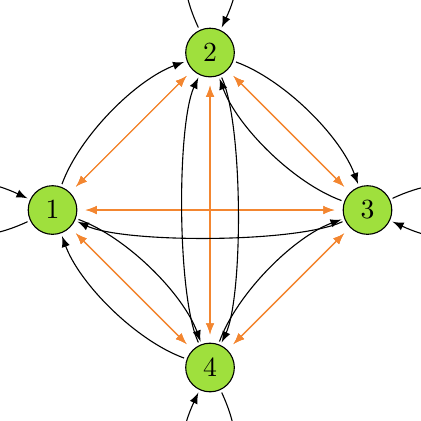
\begin{tikzpicture}
{ \definecolor{mycolor}{RGB}{159,224,61}
\node[hid, fill=mycolor] (1) at (180:2) {1};}
{ \definecolor{mycolor}{RGB}{159,224,61}
\node[hid, fill=mycolor] (2) at (90:2) {2};}
{ \definecolor{mycolor}{RGB}{159,224,61}
\node[hid, fill=mycolor] (3) at (0:2) {3};}
{ \definecolor{mycolor}{RGB}{159,224,61}
\node[hid, fill=mycolor] (4) at (-90:2) {4};}
\path[overlay,draw,pil] (1) .. controls +(205.00000:20.00000mm) and +(155.00000:20.00000mm) .. (1);
  \draw[pilip, on layer=back] (1) -- (3);
  \draw[pilip, on layer=back] (1) -- (2);
\path[overlay,draw,pil] (1) .. controls +(70.00000:10.00000mm) and +(-160.00000:10.00000mm) .. (2);
  \draw[pilip, on layer=back] (1) -- (4);
\path[overlay,draw,pil] (1) .. controls +(-20.00000:10.00000mm) and +(110.00000:10.00000mm) .. (4);
  \draw[pilip, on layer=back] (2) -- (1);
  \draw[pilip, on layer=back] (2) -- (3);
\path[overlay,draw,pil] (2) .. controls +(-20.00000:10.00000mm) and +(110.00000:10.00000mm) .. (3);
\path[overlay,draw,pil] (2) .. controls +(115.00000:20.00000mm) and +(65.00000:20.00000mm) .. (2);
  \draw[pilip, on layer=back] (2) -- (4);
\path[overlay,draw,pil] (2) .. controls +(-65.00000:10.00000mm) and +(65.00000:10.00000mm) .. (4);
  \draw[pilip, on layer=back] (3) -- (1);
\path[overlay,draw,pil] (3) .. controls +(205.00000:10.00000mm) and +(-25.00000:10.00000mm) .. (1);
\path[overlay,draw,pil] (3) .. controls +(25.00000:20.00000mm) and +(-25.00000:20.00000mm) .. (3);
  \draw[pilip, on layer=back] (3) -- (2);
\path[overlay,draw,pil] (3) .. controls +(160.00000:10.00000mm) and +(-70.00000:10.00000mm) .. (2);
  \draw[pilip, on layer=back] (3) -- (4);
  \draw[pilip, on layer=back] (4) -- (1);
\path[overlay,draw,pil] (4) .. controls +(160.00000:10.00000mm) and +(-70.00000:10.00000mm) .. (1);
  \draw[pilip, on layer=back] (4) -- (3);
\path[overlay,draw,pil] (4) .. controls +(70.00000:10.00000mm) and +(-160.00000:10.00000mm) .. (3);
  \draw[pilip, on layer=back] (4) -- (2);
\path[overlay,draw,pil] (4) .. controls +(115.00000:10.00000mm) and +(-115.00000:10.00000mm) .. (2);
\path[overlay,draw,pil] (4) .. controls +(-65.00000:20.00000mm) and +(-115.00000:20.00000mm) .. (4);

\end{tikzpicture}
};
& \node[scale=0.7](){
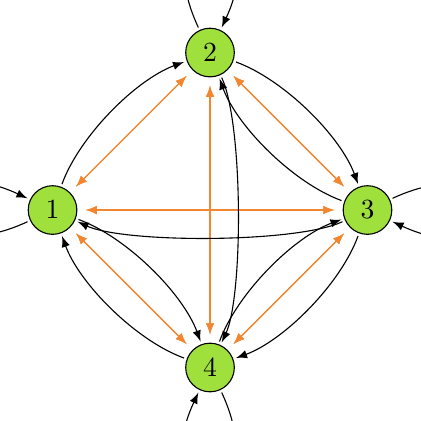
\begin{tikzpicture}
{ \definecolor{mycolor}{RGB}{159,224,61}
\node[hid, fill=mycolor] (1) at (180:2) {1};}
{ \definecolor{mycolor}{RGB}{159,224,61}
\node[hid, fill=mycolor] (2) at (90:2) {2};}
{ \definecolor{mycolor}{RGB}{159,224,61}
\node[hid, fill=mycolor] (3) at (0:2) {3};}
{ \definecolor{mycolor}{RGB}{159,224,61}
\node[hid, fill=mycolor] (4) at (-90:2) {4};}
\path[overlay,draw,pil] (1) .. controls +(205.00000:20.00000mm) and +(155.00000:20.00000mm) .. (1);
  \draw[pilip, on layer=back] (1) -- (3);
  \draw[pilip, on layer=back] (1) -- (2);
\path[overlay,draw,pil] (1) .. controls +(70.00000:10.00000mm) and +(-160.00000:10.00000mm) .. (2);
  \draw[pilip, on layer=back] (1) -- (4);
\path[overlay,draw,pil] (1) .. controls +(-20.00000:10.00000mm) and +(110.00000:10.00000mm) .. (4);
  \draw[pilip, on layer=back] (2) -- (1);
  \draw[pilip, on layer=back] (2) -- (3);
\path[overlay,draw,pil] (2) .. controls +(-20.00000:10.00000mm) and +(110.00000:10.00000mm) .. (3);
\path[overlay,draw,pil] (2) .. controls +(115.00000:20.00000mm) and +(65.00000:20.00000mm) .. (2);
  \draw[pilip, on layer=back] (2) -- (4);
\path[overlay,draw,pil] (2) .. controls +(-65.00000:10.00000mm) and +(65.00000:10.00000mm) .. (4);
  \draw[pilip, on layer=back] (3) -- (1);
\path[overlay,draw,pil] (3) .. controls +(205.00000:10.00000mm) and +(-25.00000:10.00000mm) .. (1);
\path[overlay,draw,pil] (3) .. controls +(25.00000:20.00000mm) and +(-25.00000:20.00000mm) .. (3);
  \draw[pilip, on layer=back] (3) -- (2);
\path[overlay,draw,pil] (3) .. controls +(160.00000:10.00000mm) and +(-70.00000:10.00000mm) .. (2);
  \draw[pilip, on layer=back] (3) -- (4);
\path[overlay,draw,pil] (3) .. controls +(-110.00000:10.00000mm) and +(20.00000:10.00000mm) .. (4);
  \draw[pilip, on layer=back] (4) -- (1);
\path[overlay,draw,pil] (4) .. controls +(160.00000:10.00000mm) and +(-70.00000:10.00000mm) .. (1);
  \draw[pilip, on layer=back] (4) -- (3);
\path[overlay,draw,pil] (4) .. controls +(70.00000:10.00000mm) and +(-160.00000:10.00000mm) .. (3);
  \draw[pilip, on layer=back] (4) -- (2);
\path[overlay,draw,pil] (4) .. controls +(-65.00000:20.00000mm) and +(-115.00000:20.00000mm) .. (4);

\end{tikzpicture}
};
\\
  \node[scale=0.7](){
\begin{tikzpicture}
{ \definecolor{mycolor}{RGB}{159,224,61}
\node[hid, fill=mycolor] (1) at (180:2) {1};}
{ \definecolor{mycolor}{RGB}{159,224,61}
\node[hid, fill=mycolor] (2) at (90:2) {2};}
{ \definecolor{mycolor}{RGB}{159,224,61}
\node[hid, fill=mycolor] (3) at (0:2) {3};}
{ \definecolor{mycolor}{RGB}{159,224,61}
\node[hid, fill=mycolor] (4) at (-90:2) {4};}
\path[overlay,draw,pil] (1) .. controls +(205.00000:20.00000mm) and +(155.00000:20.00000mm) .. (1);
  \draw[pilip, on layer=back] (1) -- (3);
  \draw[pilip, on layer=back] (1) -- (2);
\path[overlay,draw,pil] (1) .. controls +(70.00000:10.00000mm) and +(-160.00000:10.00000mm) .. (2);
  \draw[pilip, on layer=back] (1) -- (4);
\path[overlay,draw,pil] (1) .. controls +(-20.00000:10.00000mm) and +(110.00000:10.00000mm) .. (4);
  \draw[pilip, on layer=back] (2) -- (1);
\path[overlay,draw,pil] (2) .. controls +(-110.00000:10.00000mm) and +(20.00000:10.00000mm) .. (1);
  \draw[pilip, on layer=back] (2) -- (3);
\path[overlay,draw,pil] (2) .. controls +(-20.00000:10.00000mm) and +(110.00000:10.00000mm) .. (3);
  \draw[pilip, on layer=back] (2) -- (4);
  \draw[pilip, on layer=back] (3) -- (1);
\path[overlay,draw,pil] (3) .. controls +(205.00000:10.00000mm) and +(-25.00000:10.00000mm) .. (1);
\path[overlay,draw,pil] (3) .. controls +(25.00000:20.00000mm) and +(-25.00000:20.00000mm) .. (3);
  \draw[pilip, on layer=back] (3) -- (2);
  \draw[pilip, on layer=back] (3) -- (4);
\path[overlay,draw,pil] (3) .. controls +(-110.00000:10.00000mm) and +(20.00000:10.00000mm) .. (4);
  \draw[pilip, on layer=back] (4) -- (1);
  \draw[pilip, on layer=back] (4) -- (3);
\path[overlay,draw,pil] (4) .. controls +(70.00000:10.00000mm) and +(-160.00000:10.00000mm) .. (3);
  \draw[pilip, on layer=back] (4) -- (2);
\path[overlay,draw,pil] (4) .. controls +(115.00000:10.00000mm) and +(-115.00000:10.00000mm) .. (2);
\path[overlay,draw,pil] (4) .. controls +(-65.00000:20.00000mm) and +(-115.00000:20.00000mm) .. (4);

\end{tikzpicture}
};
& \node[scale=0.7](){
\begin{tikzpicture}
{ \definecolor{mycolor}{RGB}{61,179,224}
\node[hid, fill=mycolor] (1) at (180:2) {1};}
{ \definecolor{mycolor}{RGB}{61,179,224}
\node[hid, fill=mycolor] (2) at (90:2) {2};}
{ \definecolor{mycolor}{RGB}{159,224,61}
\node[hid, fill=mycolor] (3) at (0:2) {3};}
{ \definecolor{mycolor}{RGB}{61,179,224}
\node[hid, fill=mycolor] (4) at (-90:2) {4};}
\path[overlay,draw,pil] (1) .. controls +(205.00000:20.00000mm) and +(155.00000:20.00000mm) .. (1);
  \draw[pilip, on layer=back] (1) -- (2);
\path[overlay,draw,pil] (1) .. controls +(70.00000:10.00000mm) and +(-160.00000:10.00000mm) .. (2);
  \draw[pilip, on layer=back] (1) -- (4);
\path[overlay,draw,pil] (1) .. controls +(-20.00000:10.00000mm) and +(110.00000:10.00000mm) .. (4);
  \draw[pilip, on layer=back] (2) -- (1);
\path[overlay,draw,pil] (2) .. controls +(-110.00000:10.00000mm) and +(20.00000:10.00000mm) .. (1);
\path[overlay,draw,pil] (2) .. controls +(115.00000:20.00000mm) and +(65.00000:20.00000mm) .. (2);
  \draw[pilip, on layer=back] (2) -- (4);
\path[overlay,draw,pil] (2) .. controls +(-65.00000:10.00000mm) and +(65.00000:10.00000mm) .. (4);
\path[overlay,draw,pil] (3) .. controls +(205.00000:10.00000mm) and +(-25.00000:10.00000mm) .. (1);
\path[overlay,draw,pil] (3) .. controls +(160.00000:10.00000mm) and +(-70.00000:10.00000mm) .. (2);
\path[overlay,draw,pil] (3) .. controls +(-110.00000:10.00000mm) and +(20.00000:10.00000mm) .. (4);
  \draw[pilip, on layer=back] (4) -- (1);
\path[overlay,draw,pil] (4) .. controls +(160.00000:10.00000mm) and +(-70.00000:10.00000mm) .. (1);
  \draw[pilip, on layer=back] (4) -- (2);
\path[overlay,draw,pil] (4) .. controls +(115.00000:10.00000mm) and +(-115.00000:10.00000mm) .. (2);
\path[overlay,draw,pil] (4) .. controls +(-65.00000:20.00000mm) and +(-115.00000:20.00000mm) .. (4);

\end{tikzpicture}
};
& \node[scale=0.7](){
\begin{tikzpicture}
{ \definecolor{mycolor}{RGB}{159,224,61}
\node[hid, fill=mycolor] (1) at (180:2) {1};}
{ \definecolor{mycolor}{RGB}{159,224,61}
\node[hid, fill=mycolor] (2) at (90:2) {2};}
{ \definecolor{mycolor}{RGB}{159,224,61}
\node[hid, fill=mycolor] (3) at (0:2) {3};}
{ \definecolor{mycolor}{RGB}{159,224,61}
\node[hid, fill=mycolor] (4) at (-90:2) {4};}
\path[overlay,draw,pil] (1) .. controls +(205.00000:20.00000mm) and +(155.00000:20.00000mm) .. (1);
  \draw[pilip, on layer=back] (1) -- (3);
  \draw[pilip, on layer=back] (1) -- (2);
\path[overlay,draw,pil] (1) .. controls +(70.00000:10.00000mm) and +(-160.00000:10.00000mm) .. (2);
  \draw[pilip, on layer=back] (1) -- (4);
\path[overlay,draw,pil] (1) .. controls +(-20.00000:10.00000mm) and +(110.00000:10.00000mm) .. (4);
  \draw[pilip, on layer=back] (2) -- (1);
\path[overlay,draw,pil] (2) .. controls +(-110.00000:10.00000mm) and +(20.00000:10.00000mm) .. (1);
  \draw[pilip, on layer=back] (2) -- (3);
\path[overlay,draw,pil] (2) .. controls +(-20.00000:10.00000mm) and +(110.00000:10.00000mm) .. (3);
\path[overlay,draw,pil] (2) .. controls +(115.00000:20.00000mm) and +(65.00000:20.00000mm) .. (2);
  \draw[pilip, on layer=back] (2) -- (4);
  \draw[pilip, on layer=back] (3) -- (1);
\path[overlay,draw,pil] (3) .. controls +(205.00000:10.00000mm) and +(-25.00000:10.00000mm) .. (1);
  \draw[pilip, on layer=back] (3) -- (2);
  \draw[pilip, on layer=back] (3) -- (4);
\path[overlay,draw,pil] (3) .. controls +(-110.00000:10.00000mm) and +(20.00000:10.00000mm) .. (4);
  \draw[pilip, on layer=back] (4) -- (1);
  \draw[pilip, on layer=back] (4) -- (3);
\path[overlay,draw,pil] (4) .. controls +(70.00000:10.00000mm) and +(-160.00000:10.00000mm) .. (3);
  \draw[pilip, on layer=back] (4) -- (2);
\path[overlay,draw,pil] (4) .. controls +(115.00000:10.00000mm) and +(-115.00000:10.00000mm) .. (2);
\path[overlay,draw,pil] (4) .. controls +(-65.00000:20.00000mm) and +(-115.00000:20.00000mm) .. (4);

\end{tikzpicture}
};
& \node[scale=0.7](){
\begin{tikzpicture}
{ \definecolor{mycolor}{RGB}{159,224,61}
\node[hid, fill=mycolor] (1) at (180:2) {1};}
{ \definecolor{mycolor}{RGB}{159,224,61}
\node[hid, fill=mycolor] (2) at (90:2) {2};}
{ \definecolor{mycolor}{RGB}{159,224,61}
\node[hid, fill=mycolor] (3) at (0:2) {3};}
{ \definecolor{mycolor}{RGB}{159,224,61}
\node[hid, fill=mycolor] (4) at (-90:2) {4};}
\path[overlay,draw,pil] (1) .. controls +(205.00000:20.00000mm) and +(155.00000:20.00000mm) .. (1);
  \draw[pilip, on layer=back] (1) -- (3);
  \draw[pilip, on layer=back] (1) -- (2);
\path[overlay,draw,pil] (1) .. controls +(70.00000:10.00000mm) and +(-160.00000:10.00000mm) .. (2);
  \draw[pilip, on layer=back] (1) -- (4);
\path[overlay,draw,pil] (1) .. controls +(-20.00000:10.00000mm) and +(110.00000:10.00000mm) .. (4);
  \draw[pilip, on layer=back] (2) -- (1);
\path[overlay,draw,pil] (2) .. controls +(-110.00000:10.00000mm) and +(20.00000:10.00000mm) .. (1);
  \draw[pilip, on layer=back] (2) -- (3);
\path[overlay,draw,pil] (2) .. controls +(-20.00000:10.00000mm) and +(110.00000:10.00000mm) .. (3);
\path[overlay,draw,pil] (2) .. controls +(115.00000:20.00000mm) and +(65.00000:20.00000mm) .. (2);
  \draw[pilip, on layer=back] (2) -- (4);
  \draw[pilip, on layer=back] (3) -- (1);
\path[overlay,draw,pil] (3) .. controls +(205.00000:10.00000mm) and +(-25.00000:10.00000mm) .. (1);
\path[overlay,draw,pil] (3) .. controls +(25.00000:20.00000mm) and +(-25.00000:20.00000mm) .. (3);
  \draw[pilip, on layer=back] (3) -- (2);
  \draw[pilip, on layer=back] (3) -- (4);
\path[overlay,draw,pil] (3) .. controls +(-110.00000:10.00000mm) and +(20.00000:10.00000mm) .. (4);
  \draw[pilip, on layer=back] (4) -- (1);
  \draw[pilip, on layer=back] (4) -- (3);
\path[overlay,draw,pil] (4) .. controls +(70.00000:10.00000mm) and +(-160.00000:10.00000mm) .. (3);
  \draw[pilip, on layer=back] (4) -- (2);
\path[overlay,draw,pil] (4) .. controls +(115.00000:10.00000mm) and +(-115.00000:10.00000mm) .. (2);

\end{tikzpicture}
};
& \node[scale=0.7](){
\begin{tikzpicture}
{ \definecolor{mycolor}{RGB}{159,224,61}
\node[hid, fill=mycolor] (1) at (180:2) {1};}
{ \definecolor{mycolor}{RGB}{159,224,61}
\node[hid, fill=mycolor] (2) at (90:2) {2};}
{ \definecolor{mycolor}{RGB}{159,224,61}
\node[hid, fill=mycolor] (3) at (0:2) {3};}
{ \definecolor{mycolor}{RGB}{159,224,61}
\node[hid, fill=mycolor] (4) at (-90:2) {4};}
\path[overlay,draw,pil] (1) .. controls +(205.00000:20.00000mm) and +(155.00000:20.00000mm) .. (1);
  \draw[pilip, on layer=back] (1) -- (3);
  \draw[pilip, on layer=back] (1) -- (2);
\path[overlay,draw,pil] (1) .. controls +(70.00000:10.00000mm) and +(-160.00000:10.00000mm) .. (2);
  \draw[pilip, on layer=back] (1) -- (4);
\path[overlay,draw,pil] (1) .. controls +(-20.00000:10.00000mm) and +(110.00000:10.00000mm) .. (4);
  \draw[pilip, on layer=back] (2) -- (1);
\path[overlay,draw,pil] (2) .. controls +(-110.00000:10.00000mm) and +(20.00000:10.00000mm) .. (1);
  \draw[pilip, on layer=back] (2) -- (3);
\path[overlay,draw,pil] (2) .. controls +(-20.00000:10.00000mm) and +(110.00000:10.00000mm) .. (3);
\path[overlay,draw,pil] (2) .. controls +(115.00000:20.00000mm) and +(65.00000:20.00000mm) .. (2);
  \draw[pilip, on layer=back] (2) -- (4);
  \draw[pilip, on layer=back] (3) -- (1);
\path[overlay,draw,pil] (3) .. controls +(205.00000:10.00000mm) and +(-25.00000:10.00000mm) .. (1);
\path[overlay,draw,pil] (3) .. controls +(25.00000:20.00000mm) and +(-25.00000:20.00000mm) .. (3);
  \draw[pilip, on layer=back] (3) -- (2);
  \draw[pilip, on layer=back] (3) -- (4);
\path[overlay,draw,pil] (3) .. controls +(-110.00000:10.00000mm) and +(20.00000:10.00000mm) .. (4);
  \draw[pilip, on layer=back] (4) -- (1);
\path[overlay,draw,pil] (4) .. controls +(160.00000:10.00000mm) and +(-70.00000:10.00000mm) .. (1);
  \draw[pilip, on layer=back] (4) -- (3);
\path[overlay,draw,pil] (4) .. controls +(70.00000:10.00000mm) and +(-160.00000:10.00000mm) .. (3);
  \draw[pilip, on layer=back] (4) -- (2);
\path[overlay,draw,pil] (4) .. controls +(115.00000:10.00000mm) and +(-115.00000:10.00000mm) .. (2);
\path[overlay,draw,pil] (4) .. controls +(-65.00000:20.00000mm) and +(-115.00000:20.00000mm) .. (4);

\end{tikzpicture}
};
\\
  \node[scale=0.7](){
\begin{tikzpicture}
{ \definecolor{mycolor}{RGB}{159,224,61}
\node[hid, fill=mycolor] (1) at (180:2) {1};}
{ \definecolor{mycolor}{RGB}{159,224,61}
\node[hid, fill=mycolor] (2) at (90:2) {2};}
{ \definecolor{mycolor}{RGB}{159,224,61}
\node[hid, fill=mycolor] (3) at (0:2) {3};}
{ \definecolor{mycolor}{RGB}{159,224,61}
\node[hid, fill=mycolor] (4) at (-90:2) {4};}
\path[overlay,draw,pil] (1) .. controls +(205.00000:20.00000mm) and +(155.00000:20.00000mm) .. (1);
  \draw[pilip, on layer=back] (1) -- (3);
  \draw[pilip, on layer=back] (1) -- (2);
\path[overlay,draw,pil] (1) .. controls +(70.00000:10.00000mm) and +(-160.00000:10.00000mm) .. (2);
  \draw[pilip, on layer=back] (1) -- (4);
\path[overlay,draw,pil] (1) .. controls +(-20.00000:10.00000mm) and +(110.00000:10.00000mm) .. (4);
  \draw[pilip, on layer=back] (2) -- (1);
\path[overlay,draw,pil] (2) .. controls +(-110.00000:10.00000mm) and +(20.00000:10.00000mm) .. (1);
  \draw[pilip, on layer=back] (2) -- (3);
\path[overlay,draw,pil] (2) .. controls +(-20.00000:10.00000mm) and +(110.00000:10.00000mm) .. (3);
\path[overlay,draw,pil] (2) .. controls +(115.00000:20.00000mm) and +(65.00000:20.00000mm) .. (2);
  \draw[pilip, on layer=back] (2) -- (4);
  \draw[pilip, on layer=back] (3) -- (1);
\path[overlay,draw,pil] (3) .. controls +(205.00000:10.00000mm) and +(-25.00000:10.00000mm) .. (1);
\path[overlay,draw,pil] (3) .. controls +(25.00000:20.00000mm) and +(-25.00000:20.00000mm) .. (3);
  \draw[pilip, on layer=back] (3) -- (2);
\path[overlay,draw,pil] (3) .. controls +(160.00000:10.00000mm) and +(-70.00000:10.00000mm) .. (2);
  \draw[pilip, on layer=back] (3) -- (4);
\path[overlay,draw,pil] (3) .. controls +(-110.00000:10.00000mm) and +(20.00000:10.00000mm) .. (4);
  \draw[pilip, on layer=back] (4) -- (1);
  \draw[pilip, on layer=back] (4) -- (3);
\path[overlay,draw,pil] (4) .. controls +(70.00000:10.00000mm) and +(-160.00000:10.00000mm) .. (3);
  \draw[pilip, on layer=back] (4) -- (2);
\path[overlay,draw,pil] (4) .. controls +(115.00000:10.00000mm) and +(-115.00000:10.00000mm) .. (2);
\path[overlay,draw,pil] (4) .. controls +(-65.00000:20.00000mm) and +(-115.00000:20.00000mm) .. (4);

\end{tikzpicture}
};
& \node[scale=0.7](){
\begin{tikzpicture}
{ \definecolor{mycolor}{RGB}{159,224,61}
\node[hid, fill=mycolor] (1) at (180:2) {1};}
{ \definecolor{mycolor}{RGB}{159,224,61}
\node[hid, fill=mycolor] (2) at (90:2) {2};}
{ \definecolor{mycolor}{RGB}{159,224,61}
\node[hid, fill=mycolor] (3) at (0:2) {3};}
{ \definecolor{mycolor}{RGB}{159,224,61}
\node[hid, fill=mycolor] (4) at (-90:2) {4};}
\path[overlay,draw,pil] (1) .. controls +(205.00000:20.00000mm) and +(155.00000:20.00000mm) .. (1);
  \draw[pilip, on layer=back] (1) -- (3);
  \draw[pilip, on layer=back] (1) -- (2);
\path[overlay,draw,pil] (1) .. controls +(70.00000:10.00000mm) and +(-160.00000:10.00000mm) .. (2);
  \draw[pilip, on layer=back] (1) -- (4);
\path[overlay,draw,pil] (1) .. controls +(-20.00000:10.00000mm) and +(110.00000:10.00000mm) .. (4);
  \draw[pilip, on layer=back] (2) -- (1);
\path[overlay,draw,pil] (2) .. controls +(-110.00000:10.00000mm) and +(20.00000:10.00000mm) .. (1);
  \draw[pilip, on layer=back] (2) -- (3);
\path[overlay,draw,pil] (2) .. controls +(-20.00000:10.00000mm) and +(110.00000:10.00000mm) .. (3);
\path[overlay,draw,pil] (2) .. controls +(115.00000:20.00000mm) and +(65.00000:20.00000mm) .. (2);
  \draw[pilip, on layer=back] (2) -- (4);
\path[overlay,draw,pil] (2) .. controls +(-65.00000:10.00000mm) and +(65.00000:10.00000mm) .. (4);
  \draw[pilip, on layer=back] (3) -- (1);
\path[overlay,draw,pil] (3) .. controls +(205.00000:10.00000mm) and +(-25.00000:10.00000mm) .. (1);
\path[overlay,draw,pil] (3) .. controls +(25.00000:20.00000mm) and +(-25.00000:20.00000mm) .. (3);
  \draw[pilip, on layer=back] (3) -- (2);
  \draw[pilip, on layer=back] (3) -- (4);
\path[overlay,draw,pil] (3) .. controls +(-110.00000:10.00000mm) and +(20.00000:10.00000mm) .. (4);
  \draw[pilip, on layer=back] (4) -- (1);
  \draw[pilip, on layer=back] (4) -- (3);
\path[overlay,draw,pil] (4) .. controls +(70.00000:10.00000mm) and +(-160.00000:10.00000mm) .. (3);
  \draw[pilip, on layer=back] (4) -- (2);
\path[overlay,draw,pil] (4) .. controls +(115.00000:10.00000mm) and +(-115.00000:10.00000mm) .. (2);
\path[overlay,draw,pil] (4) .. controls +(-65.00000:20.00000mm) and +(-115.00000:20.00000mm) .. (4);

\end{tikzpicture}
};
& \node[scale=0.7](){
\begin{tikzpicture}
{ \definecolor{mycolor}{RGB}{159,224,61}
\node[hid, fill=mycolor] (1) at (180:2) {1};}
{ \definecolor{mycolor}{RGB}{159,224,61}
\node[hid, fill=mycolor] (2) at (90:2) {2};}
{ \definecolor{mycolor}{RGB}{159,224,61}
\node[hid, fill=mycolor] (3) at (0:2) {3};}
{ \definecolor{mycolor}{RGB}{159,224,61}
\node[hid, fill=mycolor] (4) at (-90:2) {4};}
\path[overlay,draw,pil] (1) .. controls +(205.00000:20.00000mm) and +(155.00000:20.00000mm) .. (1);
  \draw[pilip, on layer=back] (1) -- (3);
  \draw[pilip, on layer=back] (1) -- (2);
\path[overlay,draw,pil] (1) .. controls +(70.00000:10.00000mm) and +(-160.00000:10.00000mm) .. (2);
  \draw[pilip, on layer=back] (1) -- (4);
\path[overlay,draw,pil] (1) .. controls +(-20.00000:10.00000mm) and +(110.00000:10.00000mm) .. (4);
  \draw[pilip, on layer=back] (2) -- (1);
\path[overlay,draw,pil] (2) .. controls +(-110.00000:10.00000mm) and +(20.00000:10.00000mm) .. (1);
  \draw[pilip, on layer=back] (2) -- (3);
\path[overlay,draw,pil] (2) .. controls +(-20.00000:10.00000mm) and +(110.00000:10.00000mm) .. (3);
\path[overlay,draw,pil] (2) .. controls +(115.00000:20.00000mm) and +(65.00000:20.00000mm) .. (2);
  \draw[pilip, on layer=back] (2) -- (4);
\path[overlay,draw,pil] (2) .. controls +(-65.00000:10.00000mm) and +(65.00000:10.00000mm) .. (4);
  \draw[pilip, on layer=back] (3) -- (1);
\path[overlay,draw,pil] (3) .. controls +(205.00000:10.00000mm) and +(-25.00000:10.00000mm) .. (1);
\path[overlay,draw,pil] (3) .. controls +(25.00000:20.00000mm) and +(-25.00000:20.00000mm) .. (3);
  \draw[pilip, on layer=back] (3) -- (2);
\path[overlay,draw,pil] (3) .. controls +(160.00000:10.00000mm) and +(-70.00000:10.00000mm) .. (2);
  \draw[pilip, on layer=back] (3) -- (4);
  \draw[pilip, on layer=back] (4) -- (1);
\path[overlay,draw,pil] (4) .. controls +(160.00000:10.00000mm) and +(-70.00000:10.00000mm) .. (1);
  \draw[pilip, on layer=back] (4) -- (3);
\path[overlay,draw,pil] (4) .. controls +(70.00000:10.00000mm) and +(-160.00000:10.00000mm) .. (3);
  \draw[pilip, on layer=back] (4) -- (2);
\path[overlay,draw,pil] (4) .. controls +(-65.00000:20.00000mm) and +(-115.00000:20.00000mm) .. (4);

\end{tikzpicture}
};
& \node[scale=0.7](){
\begin{tikzpicture}
{ \definecolor{mycolor}{RGB}{159,224,61}
\node[hid, fill=mycolor] (1) at (180:2) {1};}
{ \definecolor{mycolor}{RGB}{159,224,61}
\node[hid, fill=mycolor] (2) at (90:2) {2};}
{ \definecolor{mycolor}{RGB}{159,224,61}
\node[hid, fill=mycolor] (3) at (0:2) {3};}
{ \definecolor{mycolor}{RGB}{159,224,61}
\node[hid, fill=mycolor] (4) at (-90:2) {4};}
\path[overlay,draw,pil] (1) .. controls +(205.00000:20.00000mm) and +(155.00000:20.00000mm) .. (1);
  \draw[pilip, on layer=back] (1) -- (3);
\path[overlay,draw,pil] (1) .. controls +(25.00000:10.00000mm) and +(155.00000:10.00000mm) .. (3);
  \draw[pilip, on layer=back] (1) -- (2);
\path[overlay,draw,pil] (1) .. controls +(70.00000:10.00000mm) and +(-160.00000:10.00000mm) .. (2);
  \draw[pilip, on layer=back] (1) -- (4);
  \draw[pilip, on layer=back] (2) -- (1);
  \draw[pilip, on layer=back] (2) -- (3);
\path[overlay,draw,pil] (2) .. controls +(-20.00000:10.00000mm) and +(110.00000:10.00000mm) .. (3);
  \draw[pilip, on layer=back] (2) -- (4);
\path[overlay,draw,pil] (2) .. controls +(-65.00000:10.00000mm) and +(65.00000:10.00000mm) .. (4);
  \draw[pilip, on layer=back] (3) -- (1);
\path[overlay,draw,pil] (3) .. controls +(205.00000:10.00000mm) and +(-25.00000:10.00000mm) .. (1);
\path[overlay,draw,pil] (3) .. controls +(25.00000:20.00000mm) and +(-25.00000:20.00000mm) .. (3);
  \draw[pilip, on layer=back] (3) -- (2);
  \draw[pilip, on layer=back] (3) -- (4);
\path[overlay,draw,pil] (3) .. controls +(-110.00000:10.00000mm) and +(20.00000:10.00000mm) .. (4);
  \draw[pilip, on layer=back] (4) -- (1);
\path[overlay,draw,pil] (4) .. controls +(160.00000:10.00000mm) and +(-70.00000:10.00000mm) .. (1);
  \draw[pilip, on layer=back] (4) -- (3);
  \draw[pilip, on layer=back] (4) -- (2);
\path[overlay,draw,pil] (4) .. controls +(115.00000:10.00000mm) and +(-115.00000:10.00000mm) .. (2);
\path[overlay,draw,pil] (4) .. controls +(-65.00000:20.00000mm) and +(-115.00000:20.00000mm) .. (4);

\end{tikzpicture}
};
& \node[scale=0.7](){
\begin{tikzpicture}
{ \definecolor{mycolor}{RGB}{61,179,224}
\node[hid, fill=mycolor] (1) at (180:2) {1};}
{ \definecolor{mycolor}{RGB}{240,219,62}
\node[hid, fill=mycolor] (2) at (90:2) {2};}
{ \definecolor{mycolor}{RGB}{240,219,62}
\node[hid, fill=mycolor] (3) at (0:2) {3};}
{ \definecolor{mycolor}{RGB}{159,224,61}
\node[hid, fill=mycolor] (4) at (-90:2) {4};}
\path[overlay,draw,pil] (1) .. controls +(205.00000:20.00000mm) and +(155.00000:20.00000mm) .. (1);
  \draw[pilip, on layer=back] (1) -- (3);
\path[overlay,draw,pil] (1) .. controls +(25.00000:10.00000mm) and +(155.00000:10.00000mm) .. (3);
  \draw[pilip, on layer=back] (1) -- (2);
\path[overlay,draw,pil] (1) .. controls +(70.00000:10.00000mm) and +(-160.00000:10.00000mm) .. (2);
  \draw[pilip, on layer=back] (2) -- (1);
  \draw[pilip, on layer=back] (2) -- (3);
\path[overlay,draw,pil] (2) .. controls +(-20.00000:10.00000mm) and +(110.00000:10.00000mm) .. (3);
\path[overlay,draw,pil] (2) .. controls +(115.00000:20.00000mm) and +(65.00000:20.00000mm) .. (2);
  \draw[pilip, on layer=back] (2) -- (4);
  \draw[pilip, on layer=back] (3) -- (1);
\path[overlay,draw,pil] (3) .. controls +(25.00000:20.00000mm) and +(-25.00000:20.00000mm) .. (3);
  \draw[pilip, on layer=back] (3) -- (2);
\path[overlay,draw,pil] (3) .. controls +(160.00000:10.00000mm) and +(-70.00000:10.00000mm) .. (2);
  \draw[pilip, on layer=back] (3) -- (4);
  \draw[pilip, on layer=back] (4) -- (3);
\path[overlay,draw,pil] (4) .. controls +(70.00000:10.00000mm) and +(-160.00000:10.00000mm) .. (3);
  \draw[pilip, on layer=back] (4) -- (2);
\path[overlay,draw,pil] (4) .. controls +(115.00000:10.00000mm) and +(-115.00000:10.00000mm) .. (2);
\path[overlay,draw,pil] (4) .. controls +(-65.00000:20.00000mm) and +(-115.00000:20.00000mm) .. (4);

\end{tikzpicture}
};
\\
  \node[scale=0.7](){
\begin{tikzpicture}
{ \definecolor{mycolor}{RGB}{159,224,61}
\node[hid, fill=mycolor] (1) at (180:2) {1};}
{ \definecolor{mycolor}{RGB}{159,224,61}
\node[hid, fill=mycolor] (2) at (90:2) {2};}
{ \definecolor{mycolor}{RGB}{159,224,61}
\node[hid, fill=mycolor] (3) at (0:2) {3};}
{ \definecolor{mycolor}{RGB}{159,224,61}
\node[hid, fill=mycolor] (4) at (-90:2) {4};}
\path[overlay,draw,pil] (1) .. controls +(205.00000:20.00000mm) and +(155.00000:20.00000mm) .. (1);
  \draw[pilip, on layer=back] (1) -- (3);
\path[overlay,draw,pil] (1) .. controls +(25.00000:10.00000mm) and +(155.00000:10.00000mm) .. (3);
  \draw[pilip, on layer=back] (1) -- (2);
\path[overlay,draw,pil] (1) .. controls +(70.00000:10.00000mm) and +(-160.00000:10.00000mm) .. (2);
  \draw[pilip, on layer=back] (1) -- (4);
  \draw[pilip, on layer=back] (2) -- (1);
  \draw[pilip, on layer=back] (2) -- (3);
\path[overlay,draw,pil] (2) .. controls +(-20.00000:10.00000mm) and +(110.00000:10.00000mm) .. (3);
\path[overlay,draw,pil] (2) .. controls +(115.00000:20.00000mm) and +(65.00000:20.00000mm) .. (2);
  \draw[pilip, on layer=back] (2) -- (4);
\path[overlay,draw,pil] (2) .. controls +(-65.00000:10.00000mm) and +(65.00000:10.00000mm) .. (4);
  \draw[pilip, on layer=back] (3) -- (1);
\path[overlay,draw,pil] (3) .. controls +(205.00000:10.00000mm) and +(-25.00000:10.00000mm) .. (1);
  \draw[pilip, on layer=back] (3) -- (2);
  \draw[pilip, on layer=back] (3) -- (4);
\path[overlay,draw,pil] (3) .. controls +(-110.00000:10.00000mm) and +(20.00000:10.00000mm) .. (4);
  \draw[pilip, on layer=back] (4) -- (1);
\path[overlay,draw,pil] (4) .. controls +(160.00000:10.00000mm) and +(-70.00000:10.00000mm) .. (1);
  \draw[pilip, on layer=back] (4) -- (3);
  \draw[pilip, on layer=back] (4) -- (2);
\path[overlay,draw,pil] (4) .. controls +(115.00000:10.00000mm) and +(-115.00000:10.00000mm) .. (2);
\path[overlay,draw,pil] (4) .. controls +(-65.00000:20.00000mm) and +(-115.00000:20.00000mm) .. (4);

\end{tikzpicture}
};
& \node[scale=0.7](){
\begin{tikzpicture}
{ \definecolor{mycolor}{RGB}{159,224,61}
\node[hid, fill=mycolor] (1) at (180:2) {1};}
{ \definecolor{mycolor}{RGB}{159,224,61}
\node[hid, fill=mycolor] (2) at (90:2) {2};}
{ \definecolor{mycolor}{RGB}{159,224,61}
\node[hid, fill=mycolor] (3) at (0:2) {3};}
{ \definecolor{mycolor}{RGB}{159,224,61}
\node[hid, fill=mycolor] (4) at (-90:2) {4};}
\path[overlay,draw,pil] (1) .. controls +(205.00000:20.00000mm) and +(155.00000:20.00000mm) .. (1);
  \draw[pilip, on layer=back] (1) -- (3);
\path[overlay,draw,pil] (1) .. controls +(25.00000:10.00000mm) and +(155.00000:10.00000mm) .. (3);
  \draw[pilip, on layer=back] (1) -- (2);
\path[overlay,draw,pil] (1) .. controls +(70.00000:10.00000mm) and +(-160.00000:10.00000mm) .. (2);
  \draw[pilip, on layer=back] (1) -- (4);
  \draw[pilip, on layer=back] (2) -- (1);
  \draw[pilip, on layer=back] (2) -- (3);
\path[overlay,draw,pil] (2) .. controls +(-20.00000:10.00000mm) and +(110.00000:10.00000mm) .. (3);
\path[overlay,draw,pil] (2) .. controls +(115.00000:20.00000mm) and +(65.00000:20.00000mm) .. (2);
  \draw[pilip, on layer=back] (2) -- (4);
\path[overlay,draw,pil] (2) .. controls +(-65.00000:10.00000mm) and +(65.00000:10.00000mm) .. (4);
  \draw[pilip, on layer=back] (3) -- (1);
\path[overlay,draw,pil] (3) .. controls +(205.00000:10.00000mm) and +(-25.00000:10.00000mm) .. (1);
\path[overlay,draw,pil] (3) .. controls +(25.00000:20.00000mm) and +(-25.00000:20.00000mm) .. (3);
  \draw[pilip, on layer=back] (3) -- (2);
  \draw[pilip, on layer=back] (3) -- (4);
\path[overlay,draw,pil] (3) .. controls +(-110.00000:10.00000mm) and +(20.00000:10.00000mm) .. (4);
  \draw[pilip, on layer=back] (4) -- (1);
\path[overlay,draw,pil] (4) .. controls +(160.00000:10.00000mm) and +(-70.00000:10.00000mm) .. (1);
  \draw[pilip, on layer=back] (4) -- (3);
  \draw[pilip, on layer=back] (4) -- (2);
\path[overlay,draw,pil] (4) .. controls +(115.00000:10.00000mm) and +(-115.00000:10.00000mm) .. (2);

\end{tikzpicture}
};
& \node[scale=0.7](){
\begin{tikzpicture}
{ \definecolor{mycolor}{RGB}{159,224,61}
\node[hid, fill=mycolor] (1) at (180:2) {1};}
{ \definecolor{mycolor}{RGB}{159,224,61}
\node[hid, fill=mycolor] (2) at (90:2) {2};}
{ \definecolor{mycolor}{RGB}{159,224,61}
\node[hid, fill=mycolor] (3) at (0:2) {3};}
{ \definecolor{mycolor}{RGB}{159,224,61}
\node[hid, fill=mycolor] (4) at (-90:2) {4};}
\path[overlay,draw,pil] (1) .. controls +(205.00000:20.00000mm) and +(155.00000:20.00000mm) .. (1);
  \draw[pilip, on layer=back] (1) -- (3);
\path[overlay,draw,pil] (1) .. controls +(25.00000:10.00000mm) and +(155.00000:10.00000mm) .. (3);
  \draw[pilip, on layer=back] (1) -- (2);
\path[overlay,draw,pil] (1) .. controls +(70.00000:10.00000mm) and +(-160.00000:10.00000mm) .. (2);
  \draw[pilip, on layer=back] (1) -- (4);
  \draw[pilip, on layer=back] (2) -- (1);
  \draw[pilip, on layer=back] (2) -- (3);
\path[overlay,draw,pil] (2) .. controls +(-20.00000:10.00000mm) and +(110.00000:10.00000mm) .. (3);
\path[overlay,draw,pil] (2) .. controls +(115.00000:20.00000mm) and +(65.00000:20.00000mm) .. (2);
  \draw[pilip, on layer=back] (2) -- (4);
\path[overlay,draw,pil] (2) .. controls +(-65.00000:10.00000mm) and +(65.00000:10.00000mm) .. (4);
  \draw[pilip, on layer=back] (3) -- (1);
\path[overlay,draw,pil] (3) .. controls +(205.00000:10.00000mm) and +(-25.00000:10.00000mm) .. (1);
\path[overlay,draw,pil] (3) .. controls +(25.00000:20.00000mm) and +(-25.00000:20.00000mm) .. (3);
  \draw[pilip, on layer=back] (3) -- (2);
  \draw[pilip, on layer=back] (3) -- (4);
\path[overlay,draw,pil] (3) .. controls +(-110.00000:10.00000mm) and +(20.00000:10.00000mm) .. (4);
  \draw[pilip, on layer=back] (4) -- (1);
\path[overlay,draw,pil] (4) .. controls +(160.00000:10.00000mm) and +(-70.00000:10.00000mm) .. (1);
  \draw[pilip, on layer=back] (4) -- (3);
\path[overlay,draw,pil] (4) .. controls +(70.00000:10.00000mm) and +(-160.00000:10.00000mm) .. (3);
  \draw[pilip, on layer=back] (4) -- (2);
\path[overlay,draw,pil] (4) .. controls +(115.00000:10.00000mm) and +(-115.00000:10.00000mm) .. (2);
\path[overlay,draw,pil] (4) .. controls +(-65.00000:20.00000mm) and +(-115.00000:20.00000mm) .. (4);

\end{tikzpicture}
};
& \node[scale=0.7](){
\begin{tikzpicture}
{ \definecolor{mycolor}{RGB}{159,224,61}
\node[hid, fill=mycolor] (1) at (180:2) {1};}
{ \definecolor{mycolor}{RGB}{159,224,61}
\node[hid, fill=mycolor] (2) at (90:2) {2};}
{ \definecolor{mycolor}{RGB}{159,224,61}
\node[hid, fill=mycolor] (3) at (0:2) {3};}
{ \definecolor{mycolor}{RGB}{159,224,61}
\node[hid, fill=mycolor] (4) at (-90:2) {4};}
\path[overlay,draw,pil] (1) .. controls +(205.00000:20.00000mm) and +(155.00000:20.00000mm) .. (1);
  \draw[pilip, on layer=back] (1) -- (3);
\path[overlay,draw,pil] (1) .. controls +(25.00000:10.00000mm) and +(155.00000:10.00000mm) .. (3);
  \draw[pilip, on layer=back] (1) -- (2);
\path[overlay,draw,pil] (1) .. controls +(70.00000:10.00000mm) and +(-160.00000:10.00000mm) .. (2);
  \draw[pilip, on layer=back] (1) -- (4);
  \draw[pilip, on layer=back] (2) -- (1);
  \draw[pilip, on layer=back] (2) -- (3);
\path[overlay,draw,pil] (2) .. controls +(-20.00000:10.00000mm) and +(110.00000:10.00000mm) .. (3);
\path[overlay,draw,pil] (2) .. controls +(115.00000:20.00000mm) and +(65.00000:20.00000mm) .. (2);
  \draw[pilip, on layer=back] (2) -- (4);
\path[overlay,draw,pil] (2) .. controls +(-65.00000:10.00000mm) and +(65.00000:10.00000mm) .. (4);
  \draw[pilip, on layer=back] (3) -- (1);
\path[overlay,draw,pil] (3) .. controls +(205.00000:10.00000mm) and +(-25.00000:10.00000mm) .. (1);
\path[overlay,draw,pil] (3) .. controls +(25.00000:20.00000mm) and +(-25.00000:20.00000mm) .. (3);
  \draw[pilip, on layer=back] (3) -- (2);
\path[overlay,draw,pil] (3) .. controls +(160.00000:10.00000mm) and +(-70.00000:10.00000mm) .. (2);
  \draw[pilip, on layer=back] (3) -- (4);
\path[overlay,draw,pil] (3) .. controls +(-110.00000:10.00000mm) and +(20.00000:10.00000mm) .. (4);
  \draw[pilip, on layer=back] (4) -- (1);
\path[overlay,draw,pil] (4) .. controls +(160.00000:10.00000mm) and +(-70.00000:10.00000mm) .. (1);
  \draw[pilip, on layer=back] (4) -- (3);
  \draw[pilip, on layer=back] (4) -- (2);
\path[overlay,draw,pil] (4) .. controls +(115.00000:10.00000mm) and +(-115.00000:10.00000mm) .. (2);
\path[overlay,draw,pil] (4) .. controls +(-65.00000:20.00000mm) and +(-115.00000:20.00000mm) .. (4);

\end{tikzpicture}
};
& \node[scale=0.7](){
\begin{tikzpicture}
{ \definecolor{mycolor}{RGB}{159,224,61}
\node[hid, fill=mycolor] (1) at (180:2) {1};}
{ \definecolor{mycolor}{RGB}{159,224,61}
\node[hid, fill=mycolor] (2) at (90:2) {2};}
{ \definecolor{mycolor}{RGB}{159,224,61}
\node[hid, fill=mycolor] (3) at (0:2) {3};}
{ \definecolor{mycolor}{RGB}{159,224,61}
\node[hid, fill=mycolor] (4) at (-90:2) {4};}
\path[overlay,draw,pil] (1) .. controls +(205.00000:20.00000mm) and +(155.00000:20.00000mm) .. (1);
  \draw[pilip, on layer=back] (1) -- (3);
\path[overlay,draw,pil] (1) .. controls +(25.00000:10.00000mm) and +(155.00000:10.00000mm) .. (3);
  \draw[pilip, on layer=back] (1) -- (2);
\path[overlay,draw,pil] (1) .. controls +(70.00000:10.00000mm) and +(-160.00000:10.00000mm) .. (2);
  \draw[pilip, on layer=back] (1) -- (4);
  \draw[pilip, on layer=back] (2) -- (1);
\path[overlay,draw,pil] (2) .. controls +(-110.00000:10.00000mm) and +(20.00000:10.00000mm) .. (1);
  \draw[pilip, on layer=back] (2) -- (3);
  \draw[pilip, on layer=back] (2) -- (4);
\path[overlay,draw,pil] (2) .. controls +(-65.00000:10.00000mm) and +(65.00000:10.00000mm) .. (4);
  \draw[pilip, on layer=back] (3) -- (1);
\path[overlay,draw,pil] (3) .. controls +(25.00000:20.00000mm) and +(-25.00000:20.00000mm) .. (3);
  \draw[pilip, on layer=back] (3) -- (2);
\path[overlay,draw,pil] (3) .. controls +(160.00000:10.00000mm) and +(-70.00000:10.00000mm) .. (2);
  \draw[pilip, on layer=back] (3) -- (4);
\path[overlay,draw,pil] (3) .. controls +(-110.00000:10.00000mm) and +(20.00000:10.00000mm) .. (4);
  \draw[pilip, on layer=back] (4) -- (1);
\path[overlay,draw,pil] (4) .. controls +(160.00000:10.00000mm) and +(-70.00000:10.00000mm) .. (1);
  \draw[pilip, on layer=back] (4) -- (3);
\path[overlay,draw,pil] (4) .. controls +(70.00000:10.00000mm) and +(-160.00000:10.00000mm) .. (3);
  \draw[pilip, on layer=back] (4) -- (2);
\path[overlay,draw,pil] (4) .. controls +(-65.00000:20.00000mm) and +(-115.00000:20.00000mm) .. (4);

\end{tikzpicture}
};
\\
  \node[scale=0.7](){
\begin{tikzpicture}
{ \definecolor{mycolor}{RGB}{159,224,61}
\node[hid, fill=mycolor] (1) at (180:2) {1};}
{ \definecolor{mycolor}{RGB}{159,224,61}
\node[hid, fill=mycolor] (2) at (90:2) {2};}
{ \definecolor{mycolor}{RGB}{159,224,61}
\node[hid, fill=mycolor] (3) at (0:2) {3};}
{ \definecolor{mycolor}{RGB}{159,224,61}
\node[hid, fill=mycolor] (4) at (-90:2) {4};}
\path[overlay,draw,pil] (1) .. controls +(205.00000:20.00000mm) and +(155.00000:20.00000mm) .. (1);
  \draw[pilip, on layer=back] (1) -- (3);
\path[overlay,draw,pil] (1) .. controls +(25.00000:10.00000mm) and +(155.00000:10.00000mm) .. (3);
  \draw[pilip, on layer=back] (1) -- (2);
\path[overlay,draw,pil] (1) .. controls +(70.00000:10.00000mm) and +(-160.00000:10.00000mm) .. (2);
  \draw[pilip, on layer=back] (1) -- (4);
  \draw[pilip, on layer=back] (2) -- (1);
\path[overlay,draw,pil] (2) .. controls +(-110.00000:10.00000mm) and +(20.00000:10.00000mm) .. (1);
  \draw[pilip, on layer=back] (2) -- (3);
\path[overlay,draw,pil] (2) .. controls +(115.00000:20.00000mm) and +(65.00000:20.00000mm) .. (2);
  \draw[pilip, on layer=back] (2) -- (4);
\path[overlay,draw,pil] (2) .. controls +(-65.00000:10.00000mm) and +(65.00000:10.00000mm) .. (4);
  \draw[pilip, on layer=back] (3) -- (1);
  \draw[pilip, on layer=back] (3) -- (2);
\path[overlay,draw,pil] (3) .. controls +(160.00000:10.00000mm) and +(-70.00000:10.00000mm) .. (2);
  \draw[pilip, on layer=back] (3) -- (4);
\path[overlay,draw,pil] (3) .. controls +(-110.00000:10.00000mm) and +(20.00000:10.00000mm) .. (4);
  \draw[pilip, on layer=back] (4) -- (1);
\path[overlay,draw,pil] (4) .. controls +(160.00000:10.00000mm) and +(-70.00000:10.00000mm) .. (1);
  \draw[pilip, on layer=back] (4) -- (3);
\path[overlay,draw,pil] (4) .. controls +(70.00000:10.00000mm) and +(-160.00000:10.00000mm) .. (3);
  \draw[pilip, on layer=back] (4) -- (2);
\path[overlay,draw,pil] (4) .. controls +(-65.00000:20.00000mm) and +(-115.00000:20.00000mm) .. (4);

\end{tikzpicture}
};
& \node[scale=0.7](){
\begin{tikzpicture}
{ \definecolor{mycolor}{RGB}{159,224,61}
\node[hid, fill=mycolor] (1) at (180:2) {1};}
{ \definecolor{mycolor}{RGB}{159,224,61}
\node[hid, fill=mycolor] (2) at (90:2) {2};}
{ \definecolor{mycolor}{RGB}{159,224,61}
\node[hid, fill=mycolor] (3) at (0:2) {3};}
{ \definecolor{mycolor}{RGB}{159,224,61}
\node[hid, fill=mycolor] (4) at (-90:2) {4};}
\path[overlay,draw,pil] (1) .. controls +(205.00000:20.00000mm) and +(155.00000:20.00000mm) .. (1);
  \draw[pilip, on layer=back] (1) -- (3);
\path[overlay,draw,pil] (1) .. controls +(25.00000:10.00000mm) and +(155.00000:10.00000mm) .. (3);
  \draw[pilip, on layer=back] (1) -- (2);
\path[overlay,draw,pil] (1) .. controls +(70.00000:10.00000mm) and +(-160.00000:10.00000mm) .. (2);
  \draw[pilip, on layer=back] (1) -- (4);
  \draw[pilip, on layer=back] (2) -- (1);
\path[overlay,draw,pil] (2) .. controls +(-110.00000:10.00000mm) and +(20.00000:10.00000mm) .. (1);
  \draw[pilip, on layer=back] (2) -- (3);
\path[overlay,draw,pil] (2) .. controls +(115.00000:20.00000mm) and +(65.00000:20.00000mm) .. (2);
  \draw[pilip, on layer=back] (2) -- (4);
\path[overlay,draw,pil] (2) .. controls +(-65.00000:10.00000mm) and +(65.00000:10.00000mm) .. (4);
  \draw[pilip, on layer=back] (3) -- (1);
\path[overlay,draw,pil] (3) .. controls +(25.00000:20.00000mm) and +(-25.00000:20.00000mm) .. (3);
  \draw[pilip, on layer=back] (3) -- (2);
\path[overlay,draw,pil] (3) .. controls +(160.00000:10.00000mm) and +(-70.00000:10.00000mm) .. (2);
  \draw[pilip, on layer=back] (3) -- (4);
\path[overlay,draw,pil] (3) .. controls +(-110.00000:10.00000mm) and +(20.00000:10.00000mm) .. (4);
  \draw[pilip, on layer=back] (4) -- (1);
\path[overlay,draw,pil] (4) .. controls +(160.00000:10.00000mm) and +(-70.00000:10.00000mm) .. (1);
  \draw[pilip, on layer=back] (4) -- (3);
\path[overlay,draw,pil] (4) .. controls +(70.00000:10.00000mm) and +(-160.00000:10.00000mm) .. (3);
  \draw[pilip, on layer=back] (4) -- (2);

\end{tikzpicture}
};
& \node[scale=0.7](){
\begin{tikzpicture}
{ \definecolor{mycolor}{RGB}{159,224,61}
\node[hid, fill=mycolor] (1) at (180:2) {1};}
{ \definecolor{mycolor}{RGB}{159,224,61}
\node[hid, fill=mycolor] (2) at (90:2) {2};}
{ \definecolor{mycolor}{RGB}{159,224,61}
\node[hid, fill=mycolor] (3) at (0:2) {3};}
{ \definecolor{mycolor}{RGB}{159,224,61}
\node[hid, fill=mycolor] (4) at (-90:2) {4};}
\path[overlay,draw,pil] (1) .. controls +(205.00000:20.00000mm) and +(155.00000:20.00000mm) .. (1);
  \draw[pilip, on layer=back] (1) -- (3);
\path[overlay,draw,pil] (1) .. controls +(25.00000:10.00000mm) and +(155.00000:10.00000mm) .. (3);
  \draw[pilip, on layer=back] (1) -- (2);
\path[overlay,draw,pil] (1) .. controls +(70.00000:10.00000mm) and +(-160.00000:10.00000mm) .. (2);
  \draw[pilip, on layer=back] (1) -- (4);
  \draw[pilip, on layer=back] (2) -- (1);
\path[overlay,draw,pil] (2) .. controls +(-110.00000:10.00000mm) and +(20.00000:10.00000mm) .. (1);
  \draw[pilip, on layer=back] (2) -- (3);
\path[overlay,draw,pil] (2) .. controls +(115.00000:20.00000mm) and +(65.00000:20.00000mm) .. (2);
  \draw[pilip, on layer=back] (2) -- (4);
\path[overlay,draw,pil] (2) .. controls +(-65.00000:10.00000mm) and +(65.00000:10.00000mm) .. (4);
  \draw[pilip, on layer=back] (3) -- (1);
\path[overlay,draw,pil] (3) .. controls +(25.00000:20.00000mm) and +(-25.00000:20.00000mm) .. (3);
  \draw[pilip, on layer=back] (3) -- (2);
\path[overlay,draw,pil] (3) .. controls +(160.00000:10.00000mm) and +(-70.00000:10.00000mm) .. (2);
  \draw[pilip, on layer=back] (3) -- (4);
\path[overlay,draw,pil] (3) .. controls +(-110.00000:10.00000mm) and +(20.00000:10.00000mm) .. (4);
  \draw[pilip, on layer=back] (4) -- (1);
\path[overlay,draw,pil] (4) .. controls +(160.00000:10.00000mm) and +(-70.00000:10.00000mm) .. (1);
  \draw[pilip, on layer=back] (4) -- (3);
\path[overlay,draw,pil] (4) .. controls +(70.00000:10.00000mm) and +(-160.00000:10.00000mm) .. (3);
  \draw[pilip, on layer=back] (4) -- (2);
\path[overlay,draw,pil] (4) .. controls +(115.00000:10.00000mm) and +(-115.00000:10.00000mm) .. (2);
\path[overlay,draw,pil] (4) .. controls +(-65.00000:20.00000mm) and +(-115.00000:20.00000mm) .. (4);

\end{tikzpicture}
};
& \node[scale=0.7](){
\begin{tikzpicture}
{ \definecolor{mycolor}{RGB}{159,224,61}
\node[hid, fill=mycolor] (1) at (180:2) {1};}
{ \definecolor{mycolor}{RGB}{159,224,61}
\node[hid, fill=mycolor] (2) at (90:2) {2};}
{ \definecolor{mycolor}{RGB}{159,224,61}
\node[hid, fill=mycolor] (3) at (0:2) {3};}
{ \definecolor{mycolor}{RGB}{159,224,61}
\node[hid, fill=mycolor] (4) at (-90:2) {4};}
\path[overlay,draw,pil] (1) .. controls +(205.00000:20.00000mm) and +(155.00000:20.00000mm) .. (1);
  \draw[pilip, on layer=back] (1) -- (3);
\path[overlay,draw,pil] (1) .. controls +(25.00000:10.00000mm) and +(155.00000:10.00000mm) .. (3);
  \draw[pilip, on layer=back] (1) -- (2);
\path[overlay,draw,pil] (1) .. controls +(70.00000:10.00000mm) and +(-160.00000:10.00000mm) .. (2);
  \draw[pilip, on layer=back] (1) -- (4);
  \draw[pilip, on layer=back] (2) -- (1);
\path[overlay,draw,pil] (2) .. controls +(-110.00000:10.00000mm) and +(20.00000:10.00000mm) .. (1);
  \draw[pilip, on layer=back] (2) -- (3);
\path[overlay,draw,pil] (2) .. controls +(115.00000:20.00000mm) and +(65.00000:20.00000mm) .. (2);
  \draw[pilip, on layer=back] (2) -- (4);
\path[overlay,draw,pil] (2) .. controls +(-65.00000:10.00000mm) and +(65.00000:10.00000mm) .. (4);
  \draw[pilip, on layer=back] (3) -- (1);
\path[overlay,draw,pil] (3) .. controls +(205.00000:10.00000mm) and +(-25.00000:10.00000mm) .. (1);
\path[overlay,draw,pil] (3) .. controls +(25.00000:20.00000mm) and +(-25.00000:20.00000mm) .. (3);
  \draw[pilip, on layer=back] (3) -- (2);
\path[overlay,draw,pil] (3) .. controls +(160.00000:10.00000mm) and +(-70.00000:10.00000mm) .. (2);
  \draw[pilip, on layer=back] (3) -- (4);
\path[overlay,draw,pil] (3) .. controls +(-110.00000:10.00000mm) and +(20.00000:10.00000mm) .. (4);
  \draw[pilip, on layer=back] (4) -- (1);
\path[overlay,draw,pil] (4) .. controls +(160.00000:10.00000mm) and +(-70.00000:10.00000mm) .. (1);
  \draw[pilip, on layer=back] (4) -- (3);
\path[overlay,draw,pil] (4) .. controls +(70.00000:10.00000mm) and +(-160.00000:10.00000mm) .. (3);
  \draw[pilip, on layer=back] (4) -- (2);
\path[overlay,draw,pil] (4) .. controls +(-65.00000:20.00000mm) and +(-115.00000:20.00000mm) .. (4);

\end{tikzpicture}
};
& \node[scale=0.7](){
\begin{tikzpicture}
{ \definecolor{mycolor}{RGB}{61,179,224}
\node[hid, fill=mycolor] (1) at (180:2) {1};}
{ \definecolor{mycolor}{RGB}{61,179,224}
\node[hid, fill=mycolor] (2) at (90:2) {2};}
{ \definecolor{mycolor}{RGB}{61,179,224}
\node[hid, fill=mycolor] (3) at (0:2) {3};}
{ \definecolor{mycolor}{RGB}{159,224,61}
\node[hid, fill=mycolor] (4) at (-90:2) {4};}
\path[overlay,draw,pil] (1) .. controls +(205.00000:20.00000mm) and +(155.00000:20.00000mm) .. (1);
  \draw[pilip, on layer=back] (1) -- (3);
\path[overlay,draw,pil] (1) .. controls +(25.00000:10.00000mm) and +(155.00000:10.00000mm) .. (3);
  \draw[pilip, on layer=back] (1) -- (2);
\path[overlay,draw,pil] (1) .. controls +(70.00000:10.00000mm) and +(-160.00000:10.00000mm) .. (2);
  \draw[pilip, on layer=back] (2) -- (1);
\path[overlay,draw,pil] (2) .. controls +(-110.00000:10.00000mm) and +(20.00000:10.00000mm) .. (1);
  \draw[pilip, on layer=back] (2) -- (3);
\path[overlay,draw,pil] (2) .. controls +(-20.00000:10.00000mm) and +(110.00000:10.00000mm) .. (3);
\path[overlay,draw,pil] (2) .. controls +(115.00000:20.00000mm) and +(65.00000:20.00000mm) .. (2);
  \draw[pilip, on layer=back] (3) -- (1);
\path[overlay,draw,pil] (3) .. controls +(205.00000:10.00000mm) and +(-25.00000:10.00000mm) .. (1);
\path[overlay,draw,pil] (3) .. controls +(25.00000:20.00000mm) and +(-25.00000:20.00000mm) .. (3);
  \draw[pilip, on layer=back] (3) -- (2);
\path[overlay,draw,pil] (3) .. controls +(160.00000:10.00000mm) and +(-70.00000:10.00000mm) .. (2);
\path[overlay,draw,pil] (4) .. controls +(160.00000:10.00000mm) and +(-70.00000:10.00000mm) .. (1);
\path[overlay,draw,pil] (4) .. controls +(70.00000:10.00000mm) and +(-160.00000:10.00000mm) .. (3);
\path[overlay,draw,pil] (4) .. controls +(115.00000:10.00000mm) and +(-115.00000:10.00000mm) .. (2);

\end{tikzpicture}
};
\\
  \node[scale=0.7](){
\begin{tikzpicture}
{ \definecolor{mycolor}{RGB}{159,224,61}
\node[hid, fill=mycolor] (1) at (180:2) {1};}
{ \definecolor{mycolor}{RGB}{159,224,61}
\node[hid, fill=mycolor] (2) at (90:2) {2};}
{ \definecolor{mycolor}{RGB}{159,224,61}
\node[hid, fill=mycolor] (3) at (0:2) {3};}
{ \definecolor{mycolor}{RGB}{159,224,61}
\node[hid, fill=mycolor] (4) at (-90:2) {4};}
\path[overlay,draw,pil] (1) .. controls +(205.00000:20.00000mm) and +(155.00000:20.00000mm) .. (1);
  \draw[pilip, on layer=back] (1) -- (3);
\path[overlay,draw,pil] (1) .. controls +(25.00000:10.00000mm) and +(155.00000:10.00000mm) .. (3);
  \draw[pilip, on layer=back] (1) -- (2);
\path[overlay,draw,pil] (1) .. controls +(70.00000:10.00000mm) and +(-160.00000:10.00000mm) .. (2);
  \draw[pilip, on layer=back] (1) -- (4);
  \draw[pilip, on layer=back] (2) -- (1);
\path[overlay,draw,pil] (2) .. controls +(-110.00000:10.00000mm) and +(20.00000:10.00000mm) .. (1);
  \draw[pilip, on layer=back] (2) -- (3);
\path[overlay,draw,pil] (2) .. controls +(-20.00000:10.00000mm) and +(110.00000:10.00000mm) .. (3);
\path[overlay,draw,pil] (2) .. controls +(115.00000:20.00000mm) and +(65.00000:20.00000mm) .. (2);
  \draw[pilip, on layer=back] (2) -- (4);
\path[overlay,draw,pil] (2) .. controls +(-65.00000:10.00000mm) and +(65.00000:10.00000mm) .. (4);
  \draw[pilip, on layer=back] (3) -- (1);
\path[overlay,draw,pil] (3) .. controls +(25.00000:20.00000mm) and +(-25.00000:20.00000mm) .. (3);
  \draw[pilip, on layer=back] (3) -- (2);
\path[overlay,draw,pil] (3) .. controls +(160.00000:10.00000mm) and +(-70.00000:10.00000mm) .. (2);
  \draw[pilip, on layer=back] (3) -- (4);
\path[overlay,draw,pil] (3) .. controls +(-110.00000:10.00000mm) and +(20.00000:10.00000mm) .. (4);
  \draw[pilip, on layer=back] (4) -- (1);
\path[overlay,draw,pil] (4) .. controls +(160.00000:10.00000mm) and +(-70.00000:10.00000mm) .. (1);
  \draw[pilip, on layer=back] (4) -- (3);
\path[overlay,draw,pil] (4) .. controls +(70.00000:10.00000mm) and +(-160.00000:10.00000mm) .. (3);
  \draw[pilip, on layer=back] (4) -- (2);
\path[overlay,draw,pil] (4) .. controls +(-65.00000:20.00000mm) and +(-115.00000:20.00000mm) .. (4);

\end{tikzpicture}
};
& \node[scale=0.7](){
\begin{tikzpicture}
{ \definecolor{mycolor}{RGB}{159,224,61}
\node[hid, fill=mycolor] (1) at (180:2) {1};}
{ \definecolor{mycolor}{RGB}{159,224,61}
\node[hid, fill=mycolor] (2) at (90:2) {2};}
{ \definecolor{mycolor}{RGB}{159,224,61}
\node[hid, fill=mycolor] (3) at (0:2) {3};}
{ \definecolor{mycolor}{RGB}{159,224,61}
\node[hid, fill=mycolor] (4) at (-90:2) {4};}
\path[overlay,draw,pil] (1) .. controls +(205.00000:20.00000mm) and +(155.00000:20.00000mm) .. (1);
  \draw[pilip, on layer=back] (1) -- (3);
\path[overlay,draw,pil] (1) .. controls +(25.00000:10.00000mm) and +(155.00000:10.00000mm) .. (3);
  \draw[pilip, on layer=back] (1) -- (2);
\path[overlay,draw,pil] (1) .. controls +(70.00000:10.00000mm) and +(-160.00000:10.00000mm) .. (2);
  \draw[pilip, on layer=back] (1) -- (4);
  \draw[pilip, on layer=back] (2) -- (1);
\path[overlay,draw,pil] (2) .. controls +(-110.00000:10.00000mm) and +(20.00000:10.00000mm) .. (1);
  \draw[pilip, on layer=back] (2) -- (3);
\path[overlay,draw,pil] (2) .. controls +(-20.00000:10.00000mm) and +(110.00000:10.00000mm) .. (3);
\path[overlay,draw,pil] (2) .. controls +(115.00000:20.00000mm) and +(65.00000:20.00000mm) .. (2);
  \draw[pilip, on layer=back] (2) -- (4);
\path[overlay,draw,pil] (2) .. controls +(-65.00000:10.00000mm) and +(65.00000:10.00000mm) .. (4);
  \draw[pilip, on layer=back] (3) -- (1);
\path[overlay,draw,pil] (3) .. controls +(205.00000:10.00000mm) and +(-25.00000:10.00000mm) .. (1);
\path[overlay,draw,pil] (3) .. controls +(25.00000:20.00000mm) and +(-25.00000:20.00000mm) .. (3);
  \draw[pilip, on layer=back] (3) -- (2);
  \draw[pilip, on layer=back] (3) -- (4);
\path[overlay,draw,pil] (3) .. controls +(-110.00000:10.00000mm) and +(20.00000:10.00000mm) .. (4);
  \draw[pilip, on layer=back] (4) -- (1);
\path[overlay,draw,pil] (4) .. controls +(160.00000:10.00000mm) and +(-70.00000:10.00000mm) .. (1);
  \draw[pilip, on layer=back] (4) -- (3);
  \draw[pilip, on layer=back] (4) -- (2);
\path[overlay,draw,pil] (4) .. controls +(115.00000:10.00000mm) and +(-115.00000:10.00000mm) .. (2);
\path[overlay,draw,pil] (4) .. controls +(-65.00000:20.00000mm) and +(-115.00000:20.00000mm) .. (4);

\end{tikzpicture}
};
& \node[scale=0.7](){
\begin{tikzpicture}
{ \definecolor{mycolor}{RGB}{159,224,61}
\node[hid, fill=mycolor] (1) at (180:2) {1};}
{ \definecolor{mycolor}{RGB}{61,179,224}
\node[hid, fill=mycolor] (2) at (90:2) {2};}
{ \definecolor{mycolor}{RGB}{159,224,61}
\node[hid, fill=mycolor] (3) at (0:2) {3};}
{ \definecolor{mycolor}{RGB}{159,224,61}
\node[hid, fill=mycolor] (4) at (-90:2) {4};}
\path[overlay,draw,pil] (1) .. controls +(205.00000:20.00000mm) and +(155.00000:20.00000mm) .. (1);
  \draw[pilip, on layer=back] (1) -- (3);
\path[overlay,draw,pil] (1) .. controls +(25.00000:10.00000mm) and +(155.00000:10.00000mm) .. (3);
  \draw[pilip, on layer=back] (1) -- (2);
\path[overlay,draw,pil] (1) .. controls +(70.00000:10.00000mm) and +(-160.00000:10.00000mm) .. (2);
  \draw[pilip, on layer=back] (1) -- (4);
\path[overlay,draw,pil] (1) .. controls +(-20.00000:10.00000mm) and +(110.00000:10.00000mm) .. (4);
  \draw[pilip, on layer=back] (2) -- (1);
  \draw[pilip, on layer=back] (2) -- (3);
  \draw[pilip, on layer=back] (2) -- (4);
  \draw[pilip, on layer=back] (3) -- (1);
\path[overlay,draw,pil] (3) .. controls +(205.00000:10.00000mm) and +(-25.00000:10.00000mm) .. (1);
\path[overlay,draw,pil] (3) .. controls +(25.00000:20.00000mm) and +(-25.00000:20.00000mm) .. (3);
  \draw[pilip, on layer=back] (3) -- (2);
\path[overlay,draw,pil] (3) .. controls +(160.00000:10.00000mm) and +(-70.00000:10.00000mm) .. (2);
  \draw[pilip, on layer=back] (3) -- (4);
\path[overlay,draw,pil] (3) .. controls +(-110.00000:10.00000mm) and +(20.00000:10.00000mm) .. (4);
  \draw[pilip, on layer=back] (4) -- (1);
\path[overlay,draw,pil] (4) .. controls +(160.00000:10.00000mm) and +(-70.00000:10.00000mm) .. (1);
  \draw[pilip, on layer=back] (4) -- (3);
\path[overlay,draw,pil] (4) .. controls +(70.00000:10.00000mm) and +(-160.00000:10.00000mm) .. (3);
  \draw[pilip, on layer=back] (4) -- (2);
\path[overlay,draw,pil] (4) .. controls +(115.00000:10.00000mm) and +(-115.00000:10.00000mm) .. (2);
\path[overlay,draw,pil] (4) .. controls +(-65.00000:20.00000mm) and +(-115.00000:20.00000mm) .. (4);

\end{tikzpicture}
};
& \node[scale=0.7](){
\begin{tikzpicture}
{ \definecolor{mycolor}{RGB}{159,224,61}
\node[hid, fill=mycolor] (1) at (180:2) {1};}
{ \definecolor{mycolor}{RGB}{240,219,62}
\node[hid, fill=mycolor] (2) at (90:2) {2};}
{ \definecolor{mycolor}{RGB}{231,230,222}
\node[hid, fill=mycolor] (3) at (0:2) {3};}
{ \definecolor{mycolor}{RGB}{61,179,224}
\node[hid, fill=mycolor] (4) at (-90:2) {4};}
\path[overlay,draw,pil] (1) .. controls +(205.00000:20.00000mm) and +(155.00000:20.00000mm) .. (1);
  \draw[pilip, on layer=back] (1) -- (3);
\path[overlay,draw,pil] (1) .. controls +(25.00000:10.00000mm) and +(155.00000:10.00000mm) .. (3);
  \draw[pilip, on layer=back] (1) -- (2);
\path[overlay,draw,pil] (1) .. controls +(70.00000:10.00000mm) and +(-160.00000:10.00000mm) .. (2);
  \draw[pilip, on layer=back] (1) -- (4);
\path[overlay,draw,pil] (1) .. controls +(-20.00000:10.00000mm) and +(110.00000:10.00000mm) .. (4);
  \draw[pilip, on layer=back] (2) -- (1);
  \draw[pilip, on layer=back] (2) -- (3);
\path[overlay,draw,pil] (2) .. controls +(115.00000:20.00000mm) and +(65.00000:20.00000mm) .. (2);
  \draw[pilip, on layer=back] (2) -- (4);
  \draw[pilip, on layer=back] (3) -- (1);
\path[overlay,draw,pil] (3) .. controls +(25.00000:20.00000mm) and +(-25.00000:20.00000mm) .. (3);
  \draw[pilip, on layer=back] (3) -- (2);
  \draw[pilip, on layer=back] (3) -- (4);
  \draw[pilip, on layer=back] (4) -- (1);
  \draw[pilip, on layer=back] (4) -- (3);
  \draw[pilip, on layer=back] (4) -- (2);
\path[overlay,draw,pil] (4) .. controls +(-65.00000:20.00000mm) and +(-115.00000:20.00000mm) .. (4);

\end{tikzpicture}
};
& \node[scale=0.7](){
\begin{tikzpicture}
{ \definecolor{mycolor}{RGB}{159,224,61}
\node[hid, fill=mycolor] (1) at (180:2) {1};}
{ \definecolor{mycolor}{RGB}{159,224,61}
\node[hid, fill=mycolor] (2) at (90:2) {2};}
{ \definecolor{mycolor}{RGB}{159,224,61}
\node[hid, fill=mycolor] (3) at (0:2) {3};}
{ \definecolor{mycolor}{RGB}{159,224,61}
\node[hid, fill=mycolor] (4) at (-90:2) {4};}
\path[overlay,draw,pil] (1) .. controls +(205.00000:20.00000mm) and +(155.00000:20.00000mm) .. (1);
  \draw[pilip, on layer=back] (1) -- (3);
\path[overlay,draw,pil] (1) .. controls +(25.00000:10.00000mm) and +(155.00000:10.00000mm) .. (3);
  \draw[pilip, on layer=back] (1) -- (2);
\path[overlay,draw,pil] (1) .. controls +(70.00000:10.00000mm) and +(-160.00000:10.00000mm) .. (2);
  \draw[pilip, on layer=back] (1) -- (4);
\path[overlay,draw,pil] (1) .. controls +(-20.00000:10.00000mm) and +(110.00000:10.00000mm) .. (4);
  \draw[pilip, on layer=back] (2) -- (1);
  \draw[pilip, on layer=back] (2) -- (3);
\path[overlay,draw,pil] (2) .. controls +(-20.00000:10.00000mm) and +(110.00000:10.00000mm) .. (3);
\path[overlay,draw,pil] (2) .. controls +(115.00000:20.00000mm) and +(65.00000:20.00000mm) .. (2);
  \draw[pilip, on layer=back] (2) -- (4);
\path[overlay,draw,pil] (2) .. controls +(-65.00000:10.00000mm) and +(65.00000:10.00000mm) .. (4);
  \draw[pilip, on layer=back] (3) -- (1);
\path[overlay,draw,pil] (3) .. controls +(205.00000:10.00000mm) and +(-25.00000:10.00000mm) .. (1);
\path[overlay,draw,pil] (3) .. controls +(25.00000:20.00000mm) and +(-25.00000:20.00000mm) .. (3);
  \draw[pilip, on layer=back] (3) -- (2);
  \draw[pilip, on layer=back] (3) -- (4);
\path[overlay,draw,pil] (3) .. controls +(-110.00000:10.00000mm) and +(20.00000:10.00000mm) .. (4);
  \draw[pilip, on layer=back] (4) -- (1);
\path[overlay,draw,pil] (4) .. controls +(160.00000:10.00000mm) and +(-70.00000:10.00000mm) .. (1);
  \draw[pilip, on layer=back] (4) -- (3);
  \draw[pilip, on layer=back] (4) -- (2);
\path[overlay,draw,pil] (4) .. controls +(115.00000:10.00000mm) and +(-115.00000:10.00000mm) .. (2);
\path[overlay,draw,pil] (4) .. controls +(-65.00000:20.00000mm) and +(-115.00000:20.00000mm) .. (4);

\end{tikzpicture}
};
\\
  \node[scale=0.7](){
\begin{tikzpicture}
{ \definecolor{mycolor}{RGB}{159,224,61}
\node[hid, fill=mycolor] (1) at (180:2) {1};}
{ \definecolor{mycolor}{RGB}{159,224,61}
\node[hid, fill=mycolor] (2) at (90:2) {2};}
{ \definecolor{mycolor}{RGB}{159,224,61}
\node[hid, fill=mycolor] (3) at (0:2) {3};}
{ \definecolor{mycolor}{RGB}{159,224,61}
\node[hid, fill=mycolor] (4) at (-90:2) {4};}
\path[overlay,draw,pil] (1) .. controls +(205.00000:20.00000mm) and +(155.00000:20.00000mm) .. (1);
  \draw[pilip, on layer=back] (1) -- (3);
\path[overlay,draw,pil] (1) .. controls +(25.00000:10.00000mm) and +(155.00000:10.00000mm) .. (3);
  \draw[pilip, on layer=back] (1) -- (2);
\path[overlay,draw,pil] (1) .. controls +(70.00000:10.00000mm) and +(-160.00000:10.00000mm) .. (2);
  \draw[pilip, on layer=back] (1) -- (4);
\path[overlay,draw,pil] (1) .. controls +(-20.00000:10.00000mm) and +(110.00000:10.00000mm) .. (4);
  \draw[pilip, on layer=back] (2) -- (1);
  \draw[pilip, on layer=back] (2) -- (3);
\path[overlay,draw,pil] (2) .. controls +(-20.00000:10.00000mm) and +(110.00000:10.00000mm) .. (3);
\path[overlay,draw,pil] (2) .. controls +(115.00000:20.00000mm) and +(65.00000:20.00000mm) .. (2);
  \draw[pilip, on layer=back] (2) -- (4);
\path[overlay,draw,pil] (2) .. controls +(-65.00000:10.00000mm) and +(65.00000:10.00000mm) .. (4);
  \draw[pilip, on layer=back] (3) -- (1);
\path[overlay,draw,pil] (3) .. controls +(205.00000:10.00000mm) and +(-25.00000:10.00000mm) .. (1);
\path[overlay,draw,pil] (3) .. controls +(25.00000:20.00000mm) and +(-25.00000:20.00000mm) .. (3);
  \draw[pilip, on layer=back] (3) -- (2);
\path[overlay,draw,pil] (3) .. controls +(160.00000:10.00000mm) and +(-70.00000:10.00000mm) .. (2);
  \draw[pilip, on layer=back] (3) -- (4);
  \draw[pilip, on layer=back] (4) -- (1);
\path[overlay,draw,pil] (4) .. controls +(160.00000:10.00000mm) and +(-70.00000:10.00000mm) .. (1);
  \draw[pilip, on layer=back] (4) -- (3);
\path[overlay,draw,pil] (4) .. controls +(70.00000:10.00000mm) and +(-160.00000:10.00000mm) .. (3);
  \draw[pilip, on layer=back] (4) -- (2);
\path[overlay,draw,pil] (4) .. controls +(-65.00000:20.00000mm) and +(-115.00000:20.00000mm) .. (4);

\end{tikzpicture}
};
& \node[scale=0.7](){
\begin{tikzpicture}
{ \definecolor{mycolor}{RGB}{159,224,61}
\node[hid, fill=mycolor] (1) at (180:2) {1};}
{ \definecolor{mycolor}{RGB}{159,224,61}
\node[hid, fill=mycolor] (2) at (90:2) {2};}
{ \definecolor{mycolor}{RGB}{159,224,61}
\node[hid, fill=mycolor] (3) at (0:2) {3};}
{ \definecolor{mycolor}{RGB}{159,224,61}
\node[hid, fill=mycolor] (4) at (-90:2) {4};}
\path[overlay,draw,pil] (1) .. controls +(205.00000:20.00000mm) and +(155.00000:20.00000mm) .. (1);
  \draw[pilip, on layer=back] (1) -- (3);
\path[overlay,draw,pil] (1) .. controls +(25.00000:10.00000mm) and +(155.00000:10.00000mm) .. (3);
  \draw[pilip, on layer=back] (1) -- (2);
\path[overlay,draw,pil] (1) .. controls +(70.00000:10.00000mm) and +(-160.00000:10.00000mm) .. (2);
  \draw[pilip, on layer=back] (1) -- (4);
\path[overlay,draw,pil] (1) .. controls +(-20.00000:10.00000mm) and +(110.00000:10.00000mm) .. (4);
  \draw[pilip, on layer=back] (2) -- (1);
\path[overlay,draw,pil] (2) .. controls +(-110.00000:10.00000mm) and +(20.00000:10.00000mm) .. (1);
  \draw[pilip, on layer=back] (2) -- (3);
\path[overlay,draw,pil] (2) .. controls +(115.00000:20.00000mm) and +(65.00000:20.00000mm) .. (2);
  \draw[pilip, on layer=back] (2) -- (4);
\path[overlay,draw,pil] (2) .. controls +(-65.00000:10.00000mm) and +(65.00000:10.00000mm) .. (4);
  \draw[pilip, on layer=back] (3) -- (1);
\path[overlay,draw,pil] (3) .. controls +(25.00000:20.00000mm) and +(-25.00000:20.00000mm) .. (3);
  \draw[pilip, on layer=back] (3) -- (2);
\path[overlay,draw,pil] (3) .. controls +(160.00000:10.00000mm) and +(-70.00000:10.00000mm) .. (2);
  \draw[pilip, on layer=back] (3) -- (4);
\path[overlay,draw,pil] (3) .. controls +(-110.00000:10.00000mm) and +(20.00000:10.00000mm) .. (4);
  \draw[pilip, on layer=back] (4) -- (1);
\path[overlay,draw,pil] (4) .. controls +(160.00000:10.00000mm) and +(-70.00000:10.00000mm) .. (1);
  \draw[pilip, on layer=back] (4) -- (3);
\path[overlay,draw,pil] (4) .. controls +(70.00000:10.00000mm) and +(-160.00000:10.00000mm) .. (3);
  \draw[pilip, on layer=back] (4) -- (2);
\path[overlay,draw,pil] (4) .. controls +(-65.00000:20.00000mm) and +(-115.00000:20.00000mm) .. (4);

\end{tikzpicture}
};
& \node[scale=0.7](){
\begin{tikzpicture}
{ \definecolor{mycolor}{RGB}{159,224,61}
\node[hid, fill=mycolor] (1) at (180:2) {1};}
{ \definecolor{mycolor}{RGB}{159,224,61}
\node[hid, fill=mycolor] (2) at (90:2) {2};}
{ \definecolor{mycolor}{RGB}{159,224,61}
\node[hid, fill=mycolor] (3) at (0:2) {3};}
{ \definecolor{mycolor}{RGB}{159,224,61}
\node[hid, fill=mycolor] (4) at (-90:2) {4};}
\path[overlay,draw,pil] (1) .. controls +(205.00000:20.00000mm) and +(155.00000:20.00000mm) .. (1);
  \draw[pilip, on layer=back] (1) -- (3);
\path[overlay,draw,pil] (1) .. controls +(25.00000:10.00000mm) and +(155.00000:10.00000mm) .. (3);
  \draw[pilip, on layer=back] (1) -- (2);
\path[overlay,draw,pil] (1) .. controls +(70.00000:10.00000mm) and +(-160.00000:10.00000mm) .. (2);
  \draw[pilip, on layer=back] (1) -- (4);
\path[overlay,draw,pil] (1) .. controls +(-20.00000:10.00000mm) and +(110.00000:10.00000mm) .. (4);
  \draw[pilip, on layer=back] (2) -- (1);
\path[overlay,draw,pil] (2) .. controls +(-110.00000:10.00000mm) and +(20.00000:10.00000mm) .. (1);
  \draw[pilip, on layer=back] (2) -- (3);
\path[overlay,draw,pil] (2) .. controls +(115.00000:20.00000mm) and +(65.00000:20.00000mm) .. (2);
  \draw[pilip, on layer=back] (2) -- (4);
\path[overlay,draw,pil] (2) .. controls +(-65.00000:10.00000mm) and +(65.00000:10.00000mm) .. (4);
  \draw[pilip, on layer=back] (3) -- (1);
\path[overlay,draw,pil] (3) .. controls +(205.00000:10.00000mm) and +(-25.00000:10.00000mm) .. (1);
\path[overlay,draw,pil] (3) .. controls +(25.00000:20.00000mm) and +(-25.00000:20.00000mm) .. (3);
  \draw[pilip, on layer=back] (3) -- (2);
\path[overlay,draw,pil] (3) .. controls +(160.00000:10.00000mm) and +(-70.00000:10.00000mm) .. (2);
  \draw[pilip, on layer=back] (3) -- (4);
  \draw[pilip, on layer=back] (4) -- (1);
  \draw[pilip, on layer=back] (4) -- (3);
\path[overlay,draw,pil] (4) .. controls +(70.00000:10.00000mm) and +(-160.00000:10.00000mm) .. (3);
  \draw[pilip, on layer=back] (4) -- (2);
\path[overlay,draw,pil] (4) .. controls +(115.00000:10.00000mm) and +(-115.00000:10.00000mm) .. (2);
\path[overlay,draw,pil] (4) .. controls +(-65.00000:20.00000mm) and +(-115.00000:20.00000mm) .. (4);

\end{tikzpicture}
};
& \node[scale=0.7](){
\begin{tikzpicture}
{ \definecolor{mycolor}{RGB}{159,224,61}
\node[hid, fill=mycolor] (1) at (180:2) {1};}
{ \definecolor{mycolor}{RGB}{159,224,61}
\node[hid, fill=mycolor] (2) at (90:2) {2};}
{ \definecolor{mycolor}{RGB}{159,224,61}
\node[hid, fill=mycolor] (3) at (0:2) {3};}
{ \definecolor{mycolor}{RGB}{159,224,61}
\node[hid, fill=mycolor] (4) at (-90:2) {4};}
\path[overlay,draw,pil] (1) .. controls +(205.00000:20.00000mm) and +(155.00000:20.00000mm) .. (1);
  \draw[pilip, on layer=back] (1) -- (3);
\path[overlay,draw,pil] (1) .. controls +(25.00000:10.00000mm) and +(155.00000:10.00000mm) .. (3);
  \draw[pilip, on layer=back] (1) -- (2);
\path[overlay,draw,pil] (1) .. controls +(70.00000:10.00000mm) and +(-160.00000:10.00000mm) .. (2);
  \draw[pilip, on layer=back] (1) -- (4);
\path[overlay,draw,pil] (1) .. controls +(-20.00000:10.00000mm) and +(110.00000:10.00000mm) .. (4);
  \draw[pilip, on layer=back] (2) -- (1);
\path[overlay,draw,pil] (2) .. controls +(-110.00000:10.00000mm) and +(20.00000:10.00000mm) .. (1);
  \draw[pilip, on layer=back] (2) -- (3);
\path[overlay,draw,pil] (2) .. controls +(-20.00000:10.00000mm) and +(110.00000:10.00000mm) .. (3);
\path[overlay,draw,pil] (2) .. controls +(115.00000:20.00000mm) and +(65.00000:20.00000mm) .. (2);
  \draw[pilip, on layer=back] (2) -- (4);
  \draw[pilip, on layer=back] (3) -- (1);
\path[overlay,draw,pil] (3) .. controls +(25.00000:20.00000mm) and +(-25.00000:20.00000mm) .. (3);
  \draw[pilip, on layer=back] (3) -- (2);
\path[overlay,draw,pil] (3) .. controls +(160.00000:10.00000mm) and +(-70.00000:10.00000mm) .. (2);
  \draw[pilip, on layer=back] (3) -- (4);
\path[overlay,draw,pil] (3) .. controls +(-110.00000:10.00000mm) and +(20.00000:10.00000mm) .. (4);
  \draw[pilip, on layer=back] (4) -- (1);
\path[overlay,draw,pil] (4) .. controls +(160.00000:10.00000mm) and +(-70.00000:10.00000mm) .. (1);
  \draw[pilip, on layer=back] (4) -- (3);
  \draw[pilip, on layer=back] (4) -- (2);
\path[overlay,draw,pil] (4) .. controls +(115.00000:10.00000mm) and +(-115.00000:10.00000mm) .. (2);
\path[overlay,draw,pil] (4) .. controls +(-65.00000:20.00000mm) and +(-115.00000:20.00000mm) .. (4);

\end{tikzpicture}
};
& \node[scale=0.7](){
\begin{tikzpicture}
{ \definecolor{mycolor}{RGB}{159,224,61}
\node[hid, fill=mycolor] (1) at (180:2) {1};}
{ \definecolor{mycolor}{RGB}{159,224,61}
\node[hid, fill=mycolor] (2) at (90:2) {2};}
{ \definecolor{mycolor}{RGB}{159,224,61}
\node[hid, fill=mycolor] (3) at (0:2) {3};}
{ \definecolor{mycolor}{RGB}{159,224,61}
\node[hid, fill=mycolor] (4) at (-90:2) {4};}
\path[overlay,draw,pil] (1) .. controls +(205.00000:20.00000mm) and +(155.00000:20.00000mm) .. (1);
  \draw[pilip, on layer=back] (1) -- (3);
\path[overlay,draw,pil] (1) .. controls +(25.00000:10.00000mm) and +(155.00000:10.00000mm) .. (3);
  \draw[pilip, on layer=back] (1) -- (2);
\path[overlay,draw,pil] (1) .. controls +(70.00000:10.00000mm) and +(-160.00000:10.00000mm) .. (2);
  \draw[pilip, on layer=back] (1) -- (4);
\path[overlay,draw,pil] (1) .. controls +(-20.00000:10.00000mm) and +(110.00000:10.00000mm) .. (4);
  \draw[pilip, on layer=back] (2) -- (1);
\path[overlay,draw,pil] (2) .. controls +(-110.00000:10.00000mm) and +(20.00000:10.00000mm) .. (1);
  \draw[pilip, on layer=back] (2) -- (3);
\path[overlay,draw,pil] (2) .. controls +(-20.00000:10.00000mm) and +(110.00000:10.00000mm) .. (3);
\path[overlay,draw,pil] (2) .. controls +(115.00000:20.00000mm) and +(65.00000:20.00000mm) .. (2);
  \draw[pilip, on layer=back] (2) -- (4);
  \draw[pilip, on layer=back] (3) -- (1);
\path[overlay,draw,pil] (3) .. controls +(205.00000:10.00000mm) and +(-25.00000:10.00000mm) .. (1);
\path[overlay,draw,pil] (3) .. controls +(25.00000:20.00000mm) and +(-25.00000:20.00000mm) .. (3);
  \draw[pilip, on layer=back] (3) -- (2);
  \draw[pilip, on layer=back] (3) -- (4);
\path[overlay,draw,pil] (3) .. controls +(-110.00000:10.00000mm) and +(20.00000:10.00000mm) .. (4);
  \draw[pilip, on layer=back] (4) -- (1);
  \draw[pilip, on layer=back] (4) -- (3);
\path[overlay,draw,pil] (4) .. controls +(70.00000:10.00000mm) and +(-160.00000:10.00000mm) .. (3);
  \draw[pilip, on layer=back] (4) -- (2);
\path[overlay,draw,pil] (4) .. controls +(115.00000:10.00000mm) and +(-115.00000:10.00000mm) .. (2);
\path[overlay,draw,pil] (4) .. controls +(-65.00000:20.00000mm) and +(-115.00000:20.00000mm) .. (4);

\end{tikzpicture}
};
\\
  \node[scale=0.7](){
\begin{tikzpicture}
{ \definecolor{mycolor}{RGB}{159,224,61}
\node[hid, fill=mycolor] (1) at (180:2) {1};}
{ \definecolor{mycolor}{RGB}{159,224,61}
\node[hid, fill=mycolor] (2) at (90:2) {2};}
{ \definecolor{mycolor}{RGB}{61,179,224}
\node[hid, fill=mycolor] (3) at (0:2) {3};}
{ \definecolor{mycolor}{RGB}{159,224,61}
\node[hid, fill=mycolor] (4) at (-90:2) {4};}
\path[overlay,draw,pil] (1) .. controls +(205.00000:20.00000mm) and +(155.00000:20.00000mm) .. (1);
  \draw[pilip, on layer=back] (1) -- (3);
\path[overlay,draw,pil] (1) .. controls +(25.00000:10.00000mm) and +(155.00000:10.00000mm) .. (3);
  \draw[pilip, on layer=back] (1) -- (2);
\path[overlay,draw,pil] (1) .. controls +(70.00000:10.00000mm) and +(-160.00000:10.00000mm) .. (2);
  \draw[pilip, on layer=back] (1) -- (4);
\path[overlay,draw,pil] (1) .. controls +(-20.00000:10.00000mm) and +(110.00000:10.00000mm) .. (4);
  \draw[pilip, on layer=back] (2) -- (1);
\path[overlay,draw,pil] (2) .. controls +(-110.00000:10.00000mm) and +(20.00000:10.00000mm) .. (1);
  \draw[pilip, on layer=back] (2) -- (3);
\path[overlay,draw,pil] (2) .. controls +(-20.00000:10.00000mm) and +(110.00000:10.00000mm) .. (3);
\path[overlay,draw,pil] (2) .. controls +(115.00000:20.00000mm) and +(65.00000:20.00000mm) .. (2);
  \draw[pilip, on layer=back] (2) -- (4);
\path[overlay,draw,pil] (2) .. controls +(-65.00000:10.00000mm) and +(65.00000:10.00000mm) .. (4);
  \draw[pilip, on layer=back] (3) -- (1);
  \draw[pilip, on layer=back] (3) -- (2);
  \draw[pilip, on layer=back] (3) -- (4);
  \draw[pilip, on layer=back] (4) -- (1);
\path[overlay,draw,pil] (4) .. controls +(160.00000:10.00000mm) and +(-70.00000:10.00000mm) .. (1);
  \draw[pilip, on layer=back] (4) -- (3);
\path[overlay,draw,pil] (4) .. controls +(70.00000:10.00000mm) and +(-160.00000:10.00000mm) .. (3);
  \draw[pilip, on layer=back] (4) -- (2);
\path[overlay,draw,pil] (4) .. controls +(115.00000:10.00000mm) and +(-115.00000:10.00000mm) .. (2);
\path[overlay,draw,pil] (4) .. controls +(-65.00000:20.00000mm) and +(-115.00000:20.00000mm) .. (4);

\end{tikzpicture}
};
& \node[scale=0.7](){
\begin{tikzpicture}
{ \definecolor{mycolor}{RGB}{159,224,61}
\node[hid, fill=mycolor] (1) at (180:2) {1};}
{ \definecolor{mycolor}{RGB}{159,224,61}
\node[hid, fill=mycolor] (2) at (90:2) {2};}
{ \definecolor{mycolor}{RGB}{159,224,61}
\node[hid, fill=mycolor] (3) at (0:2) {3};}
{ \definecolor{mycolor}{RGB}{61,179,224}
\node[hid, fill=mycolor] (4) at (-90:2) {4};}
\path[overlay,draw,pil] (1) .. controls +(205.00000:20.00000mm) and +(155.00000:20.00000mm) .. (1);
  \draw[pilip, on layer=back] (1) -- (3);
\path[overlay,draw,pil] (1) .. controls +(25.00000:10.00000mm) and +(155.00000:10.00000mm) .. (3);
  \draw[pilip, on layer=back] (1) -- (2);
\path[overlay,draw,pil] (1) .. controls +(70.00000:10.00000mm) and +(-160.00000:10.00000mm) .. (2);
  \draw[pilip, on layer=back] (1) -- (4);
\path[overlay,draw,pil] (1) .. controls +(-20.00000:10.00000mm) and +(110.00000:10.00000mm) .. (4);
  \draw[pilip, on layer=back] (2) -- (1);
\path[overlay,draw,pil] (2) .. controls +(-110.00000:10.00000mm) and +(20.00000:10.00000mm) .. (1);
  \draw[pilip, on layer=back] (2) -- (3);
\path[overlay,draw,pil] (2) .. controls +(-20.00000:10.00000mm) and +(110.00000:10.00000mm) .. (3);
\path[overlay,draw,pil] (2) .. controls +(115.00000:20.00000mm) and +(65.00000:20.00000mm) .. (2);
  \draw[pilip, on layer=back] (2) -- (4);
\path[overlay,draw,pil] (2) .. controls +(-65.00000:10.00000mm) and +(65.00000:10.00000mm) .. (4);
  \draw[pilip, on layer=back] (3) -- (1);
\path[overlay,draw,pil] (3) .. controls +(205.00000:10.00000mm) and +(-25.00000:10.00000mm) .. (1);
\path[overlay,draw,pil] (3) .. controls +(25.00000:20.00000mm) and +(-25.00000:20.00000mm) .. (3);
  \draw[pilip, on layer=back] (3) -- (2);
\path[overlay,draw,pil] (3) .. controls +(160.00000:10.00000mm) and +(-70.00000:10.00000mm) .. (2);
  \draw[pilip, on layer=back] (3) -- (4);
\path[overlay,draw,pil] (3) .. controls +(-110.00000:10.00000mm) and +(20.00000:10.00000mm) .. (4);
  \draw[pilip, on layer=back] (4) -- (1);
  \draw[pilip, on layer=back] (4) -- (3);
  \draw[pilip, on layer=back] (4) -- (2);

\end{tikzpicture}
};
& \node[scale=0.7](){
\begin{tikzpicture}
{ \definecolor{mycolor}{RGB}{159,224,61}
\node[hid, fill=mycolor] (1) at (180:2) {1};}
{ \definecolor{mycolor}{RGB}{159,224,61}
\node[hid, fill=mycolor] (2) at (90:2) {2};}
{ \definecolor{mycolor}{RGB}{159,224,61}
\node[hid, fill=mycolor] (3) at (0:2) {3};}
{ \definecolor{mycolor}{RGB}{159,224,61}
\node[hid, fill=mycolor] (4) at (-90:2) {4};}
\path[overlay,draw,pil] (1) .. controls +(205.00000:20.00000mm) and +(155.00000:20.00000mm) .. (1);
  \draw[pilip, on layer=back] (1) -- (3);
\path[overlay,draw,pil] (1) .. controls +(25.00000:10.00000mm) and +(155.00000:10.00000mm) .. (3);
  \draw[pilip, on layer=back] (1) -- (2);
\path[overlay,draw,pil] (1) .. controls +(70.00000:10.00000mm) and +(-160.00000:10.00000mm) .. (2);
  \draw[pilip, on layer=back] (1) -- (4);
\path[overlay,draw,pil] (1) .. controls +(-20.00000:10.00000mm) and +(110.00000:10.00000mm) .. (4);
  \draw[pilip, on layer=back] (2) -- (1);
\path[overlay,draw,pil] (2) .. controls +(-110.00000:10.00000mm) and +(20.00000:10.00000mm) .. (1);
  \draw[pilip, on layer=back] (2) -- (3);
\path[overlay,draw,pil] (2) .. controls +(-20.00000:10.00000mm) and +(110.00000:10.00000mm) .. (3);
\path[overlay,draw,pil] (2) .. controls +(115.00000:20.00000mm) and +(65.00000:20.00000mm) .. (2);
  \draw[pilip, on layer=back] (2) -- (4);
\path[overlay,draw,pil] (2) .. controls +(-65.00000:10.00000mm) and +(65.00000:10.00000mm) .. (4);
  \draw[pilip, on layer=back] (3) -- (1);
\path[overlay,draw,pil] (3) .. controls +(205.00000:10.00000mm) and +(-25.00000:10.00000mm) .. (1);
\path[overlay,draw,pil] (3) .. controls +(25.00000:20.00000mm) and +(-25.00000:20.00000mm) .. (3);
  \draw[pilip, on layer=back] (3) -- (2);
\path[overlay,draw,pil] (3) .. controls +(160.00000:10.00000mm) and +(-70.00000:10.00000mm) .. (2);
  \draw[pilip, on layer=back] (3) -- (4);
\path[overlay,draw,pil] (3) .. controls +(-110.00000:10.00000mm) and +(20.00000:10.00000mm) .. (4);
  \draw[pilip, on layer=back] (4) -- (1);
\path[overlay,draw,pil] (4) .. controls +(160.00000:10.00000mm) and +(-70.00000:10.00000mm) .. (1);
  \draw[pilip, on layer=back] (4) -- (3);
\path[overlay,draw,pil] (4) .. controls +(70.00000:10.00000mm) and +(-160.00000:10.00000mm) .. (3);
  \draw[pilip, on layer=back] (4) -- (2);
\path[overlay,draw,pil] (4) .. controls +(115.00000:10.00000mm) and +(-115.00000:10.00000mm) .. (2);
\path[overlay,draw,pil] (4) .. controls +(-65.00000:20.00000mm) and +(-115.00000:20.00000mm) .. (4);

\end{tikzpicture}
};
\\
};

    %\input{|'compile.sh'}
  \end{tikzpicture}
\end{page}
\end{document}

%%% Local Variables:
%%% LaTeX-command: "pdflatex --shell-escape --enable-pipes"
%%% End:
